
\PassOptionsToPackage{unicode}{hyperref}
\PassOptionsToPackage{hyphens}{url}

\documentclass[]{article}
\usepackage{lmodern}

\usepackage{amsmath, amsthm, amssymb, amsfonts, amsxtra, amscd, mathtools}

\usepackage{tikz}
\usetikzlibrary{cd}

\usepackage{ifxetex,ifluatex}

\usepackage{bookmark}
\usepackage{hyperref}
\usepackage{xcolor}
\urlstyle{same} % disable monospaced font for URLs

\hypersetup{
    pdftitle={UGA Real Analysis Qualifying Exam Questions}
    colorlinks,
    linktoc=all,    
    citecolor=blue,
    filecolor=blue,
    linkcolor=blue,
    urlcolor=blue
}
\ifnum 0\ifxetex 1\fi\ifluatex 1\fi=0 % if pdftex
  \usepackage[T1]{fontenc}
  \usepackage[utf8]{inputenc}
  \usepackage{textcomp} % provide euro and other symbols
\else % if luatex or xetex
  \usepackage{unicode-math}
  \defaultfontfeatures{Scale=MatchLowercase}
  \defaultfontfeatures[\rmfamily]{Ligatures=TeX,Scale=1}
\fi

% Use upquote if available, for straight quotes in verbatim environments
\IfFileExists{upquote.sty}{\usepackage{upquote}}{}
\IfFileExists{microtype.sty}{% use microtype if available
  \usepackage[]{microtype}
  \UseMicrotypeSet[protrusion]{basicmath} % disable protrusion for tt fonts
}{}

\makeatletter
\@ifundefined{KOMAClassName}{% if non-KOMA class
  \IfFileExists{parskip.sty}{%
    \usepackage{parskip}
  }{% else
    \setlength{\parindent}{0pt}
    \setlength{\parskip}{6pt plus 2pt minus 1pt}}
}{% if KOMA class
  \KOMAoptions{parskip=half}}
\makeatother

\setlength{\emergencystretch}{3em} % prevent overfull lines
\providecommand{\tightlist}{%
  \setlength{\itemsep}{0pt}\setlength{\parskip}{0pt}
}


% Highlight quote
\usepackage{xcolor}
\usepackage{environ}
\definecolor{block-gray}{gray}{0.85}
\NewEnviron{myblock}
{\colorbox{block-gray}{%
\parbox{\dimexpr\linewidth-2\fboxsep\relax}{%
\small\addtolength{\leftskip}{10mm}
\addtolength{\rightskip}{10mm}
\BODY}}
}
\renewcommand{\quote}{\myblock}
\renewcommand{\endquote}{\endmyblock}

\newtheoremstyle{break}% name
  {}%         Space above, empty = `usual value'
  {2em}%         Space below
  {\normalfont}% Body font
  {}%         Indent amount (empty = no indent, \parindent = para indent)
  {\bfseries}% Thm head font
  {.}%        Punctuation after thm head
  {\newline}% Space after thm head: \newline = linebreak
  {}%         Thm head spec

\usepackage{chngcntr}

\newtheorem{problem}{Problem}[section]
\counterwithin*{problem}{section}

\newtheorem{solution}{Solution}[section]



\let\Begin\begin
\let\End\end
\newcommand\wrapenv[1]{#1}

\makeatletter
\def\ScaleWidthIfNeeded{%
 \ifdim\Gin@nat@width>\linewidth
    \linewidth
  \else
    \Gin@nat@width
  \fi
}
\def\ScaleHeightIfNeeded{%
  \ifdim\Gin@nat@height>0.9\textheight
    0.9\textheight
  \else
    \Gin@nat@width
  \fi
}
\makeatother

\setkeys{Gin}{width=\ScaleWidthIfNeeded,height=\ScaleHeightIfNeeded,keepaspectratio}%
% Create indices up front
\makeindex[title=Concept index]

\title{
\textbf{
    Real Analysis Qualifying Exam Questions
  }
  }

\author{D. Zack Garza}

\date{\today}






\begin{document}
\maketitle
\tableofcontents

\newpage
\listoftodos


\hypertarget{undergraduate-analysis-uniform-convergence}{%
\section{Undergraduate Analysis: Uniform
Convergence}\label{undergraduate-analysis-uniform-convergence}}

\hypertarget{fall-2018-1-bowtie}{%
\subsection{\texorpdfstring{Fall 2018 \# 1
\(\bowtie\)}{Fall 2018 \# 1 \textbackslash bowtie}}\label{fall-2018-1-bowtie}}

Let \(f(x) = \frac 1 x\). Show that \(f\) is uniformly continuous on
\((1, \infty)\) but not on \((0,\infty)\).

\begin{solution}

\begin{theorem}[asdsads]

asdsadasdas

\end{theorem}

Concepts used:

\begin{itemize}
\tightlist
\item
  Uniform continuity.
\end{itemize}

\textbf{Solution}:

\begin{itemize}
\item
  Show a stronger statement: \(f(x) = \frac 1 x\) is uniformly
  continuous on any interval of the form \((c, \infty)\) where
  \(c > 0\).
\item
  Note that
  \begin{align*}
  \abs{x}, \abs y > c > 0 \implies \abs{xy} = \abs{x}\abs{y} > c^2 \implies \frac{1}{\abs{xy}} < \frac 1 {c^{2}}
  .\end{align*}
\item
  Letting \(\varepsilon\) be arbitrary, choose
  \(\delta < \varepsilon c^2\).
\item
  Note that \(\delta\) does not depend on \(x, y\).
\item
  Then
  \begin{align*}
  \abs{f(x) - f(y)}
  &= \abs{\frac 1 x - \frac 1 y} \\
  &= \frac{\abs{x-y}}{xy} \\
  &\leq \frac{\delta}{xy} \\
  &< \frac{\delta}{c^2} \\
  &< \varepsilon
  ,\end{align*} which shows uniform continuity.
\end{itemize}

To see that \(f\) is not uniformly continuous when \(c=0\):

\begin{quote}
Note: negating uniform continuity says \(\exists \eps > 0\) such that
\(\forall \delta(\eps)\) there exist \(x, y\) such that
\(\abs{x-y} < \delta\) \emph{and} \(\abs{f(x) - f(y)} > \eps\).
\end{quote}

\begin{itemize}
\tightlist
\item
  Let \(\varepsilon < 1\).
\item
  Let \(x_n = \frac 1 n\) for \(n\geq 1\).
\item
  Choose \(n\) large enough such that
  \(\abs{x_n - x_{n+1}} = \frac 1 n - \frac 1 {n+1} < \delta\).

  \begin{itemize}
  \tightlist
  \item
    Why this can be done: by the archimedean property of \(\RR\), choose
    \(n\) such that \({1\over n} < \eps\).
  \item
    Then
    \begin{align*}
    {1 \over n} - {1\over n+1} = {1 \over n(n+1)} \leq {1\over n} < \eps \quad\text{since }n+1 > 1
    .\end{align*}
  \end{itemize}
\item
  Note \(f(x_n) = n\) and thus
  \begin{align*}\abs{f(x_n) - f(x_{n+1})} = n - (n+1) = 1 > \varepsilon.\end{align*}
\end{itemize}

\end{solution}

\hypertarget{fall-2017-1}{%
\subsection{Fall 2017 \# 1}\label{fall-2017-1}}

Let
\begin{align*}
f(x) = s \sum _{n=0}^{\infty} \frac{x^{n}}{n !}.
\end{align*}

Describe the intervals on which \(f\) does and does not converge
uniformly.

\todo[inline]{Review and consolidate.}

\begin{solution}

Concepts used:

\begin{itemize}
\tightlist
\item
  ??
\end{itemize}

\textbf{Solution}:

Note that \(f(x) = e^x\) is entire and thus equal to its power series.
So \(f(x) = \sum_{j=0}^\infty \frac 1 {j!}x^j\).

Letting \(f_N(x) = \sum_{j=1}^N \frac 1 {j!} x^j\), we have
\(f_N(x) \to f(x)\) pointwise on \((-\infty ,\infty)\).

For any compact interval \([-M, M]\), we have

\begin{align*}
\norm{f_N(x) - f(x)}_\infty
&= \sup_{-M\leq x \leq M} ~\abs{\sum_{j=N+1}^\infty \frac 1 {j!} x^j} \\
&\leq \sup_{-M\leq x \leq M} ~ \sum_{j=N+1}^\infty \frac 1 {j!} \abs{x}^j \\
&\leq \sum_{j=N+1}^\infty \frac 1 {j!} M^j \\
&\leq \sum_{j=0}^\infty \frac 1 {j!} M^j \\
&= e^M \\
&<\infty
,\end{align*}

so \(f_N \to f\) uniformly on \([-M, M]\) by the M-test. Thus it
converges on any bounded interval.

It does not converge on \(\RR\), since \(x^N\) is unbounded.

\end{solution}

\hypertarget{fall-2014-1}{%
\subsection{Fall 2014 \# 1}\label{fall-2014-1}}

Let \(\theset{f_n}\) be a sequence of continuous functions such that
\(\sum f_n\) converges uniformly.

Prove that \(\sum f_n\) is also continuous.

\hypertarget{spring-2017-4}{%
\subsection{Spring 2017 \# 4}\label{spring-2017-4}}

Let \(f(x, y)\) on \([-1, 1]^2\) be defined by
\begin{align*}
f(x, y) = \begin{cases}
\frac{x y}{\left(x^{2}+y^{2}\right)^{2}} & (x, y) \neq (0, 0) \\
0 & (x, y) = (0, 0)
\end{cases}
\end{align*} Determine if \(f\) is integrable.

\todo[inline]{Redo, may just be wrong.}

\begin{solution}

Concepts used:

\begin{itemize}
\tightlist
\item
  ??
\end{itemize}

\textbf{Solution}:

Switching to polar coordinates and integrating over a half-circle
contained in \(I^2\), we have
\begin{align*}
\int_{I^2} f \geq \int_0^\pi \int_0^1 \frac{\cos(\theta)\sin(\theta)}{r^2} ~dr~d\theta = \infty
,\end{align*}

so \(f\) is not integrable.

\end{solution}

\hypertarget{spring-2015-1}{%
\subsection{Spring 2015 \# 1}\label{spring-2015-1}}

Let \((X, d)\) and \((Y, \rho)\) be metric spaces, \(f: X\to Y\), and
\(x_0 \in X\).

Prove that the following statements are equivalent:

\begin{enumerate}
\def\labelenumi{\arabic{enumi}.}
\tightlist
\item
  For every \(\varepsilon > 0 \quad \exists \delta > 0\) such that
  \(\rho( f(x), f(x_0) ) < \varepsilon\) whenever
  \(d(x, x_0) < \delta\).
\item
  The sequence \(\theset{f(x_n)}_{n=1}^\infty \to f(x_0)\) for every
  sequence \(\theset{x_n} \to x_0\) in \(X\).
\end{enumerate}

\hypertarget{fall-2014-2}{%
\subsection{Fall 2014 \# 2}\label{fall-2014-2}}

Let \(I\) be an index set and \(\alpha: I \to (0, \infty)\).

\begin{enumerate}
\def\labelenumi{\arabic{enumi}.}
\item
  Show that
  \begin{align*}
  \sum_{i \in I} a(i):=\sup _{\substack{ J \subset I \\ J \text { finite }}} \sum_{i \in J} a(i)<\infty \implies I \text{ is countable.}
  \end{align*}
\item
  Suppose \(I = \QQ\) and \(\sum_{q \in \mathbb{Q}} a(q)<\infty\).
  Define
  \begin{align*}
    f(x):=\sum_{\substack{q \in \mathbb{Q}\\ q \leq x}} a(q).
    \end{align*} Show that \(f\) is continuous at
  \(x \iff x\not\in \QQ\).
\end{enumerate}

\hypertarget{spring-2014-2}{%
\subsection{Spring 2014 \# 2}\label{spring-2014-2}}

Let \(\theset{a_n}\) be a sequence of real numbers such that
\begin{align*}
\theset{b_n} \in \ell^2(\NN) \implies \sum a_n b_n < \infty.
\end{align*} Show that \(\sum a_n^2 < \infty\).

\begin{quote}
Note: Assume \(a_n, b_n\) are all non-negative.
\end{quote}

\hypertarget{general-analysis}{%
\section{General Analysis}\label{general-analysis}}

\hypertarget{spring-2020-1}{%
\subsection{Spring 2020 \# 1}\label{spring-2020-1}}

Prove that if \(f: [0, 1] \to \RR\) is continuous then
\begin{align*}
\lim_{k\to\infty} \int_0^1 kx^{k-1} f(x) \,dx = f(1)
.\end{align*}

\begin{solution}

Concepts used:

\begin{itemize}
\tightlist
\item
  DCT
\item
  Weierstrass Approximation Theorem
\end{itemize}

\textbf{Solution}:

\begin{itemize}
\item
  Suppose \(p\) is a polynomial, then
  \begin{align*}
  \lim_{k\to\infty} \int_0^1 kx^{k-1} p(x) \, dx
  &= \lim_{k\to\infty} \int_0^1 \qty{ \dd{}{x}x^k } p(x) \, dx \\
  &= \lim_{k\to\infty} \left[ x^k p(x) \evalfrom_0^1 - \int_0^1 x^k \qty{\dd{}{x} p(x) } \, dx \right] \quad\text{integrating by parts}\\
  &= p(1) - \lim_{k\to\infty} \int_0^1 x^k \qty{\dd{}{x} p(x) } \, dx
  ,\end{align*}
\item
  Thus it suffices to show that
  \begin{align*}
  \lim_{k\to\infty} \int_0^1 x^k \qty{\dd{}{x} p(x) } \, dx = 0
  .\end{align*}
\item
  Integrating by parts a second time yields
  \begin{align*}
  \lim_{k\to\infty} 
  \int_0^1 x^k \qty{\dd{}{x} p(x) } \, dx
  &= \lim_{k\to\infty} 
  {x^{k+1} \over k+1} p'(x) \evalfrom_0^1 - \int_0^1 {x^{k+1} \over k+1} \qty{ \dd{^2}{x^2}p(x)} \, dx \\
  &= - \lim_{k\to\infty} \int_0^1 {x^{k+1} \over k+1} \qty{ \dd{^2}{x^2}p(x)} \, dx \\
  &= - \int_0^1 \lim_{k\to\infty}  {x^{k+1} \over k+1} \qty{ \dd{^2}{x^2}p(x)} \, dx \quad\text{by DCT} \\
  &= - \int_0^1 0 \qty{ \dd{^2}{x^2}p(x)} \, dx \\
  &= 0
  .\end{align*}

  \begin{itemize}
  \tightlist
  \item
    The DCT can be applied here because \(f''\) is continuous and
    \([0, 1]\) is compact, so \(f''\) is bounded on \([0, 1]\) by a
    constant \(M\) and
    \begin{align*}\int_0^1 \abs{x^k f''(x)} \leq \int_0^1 1\cdot M = M < \infty.\end{align*}
  \end{itemize}
\item
  Now use the Weierstrass approximation theorem:

  \begin{itemize}
  \tightlist
  \item
    If \(f: [a, b] \to \RR\) is continuous, then for every \(\eps>0\)
    there exists a polynomial \(p_\eps(x)\) such that
    \(\norm{f - p_\eps}_\infty < \eps\).
  \end{itemize}
\item
  Thus
  \begin{align*}
  \abs{ \int_0^1 kx^{k-1} p_\eps(x)\,dx - \int_0^1 kx^{k-1}f(x)\,dx  } 
  &= \abs{ \int_0^1 kx^{k-1} \qty{p_\eps(x) - f(x)} \,dx  } \\
  &\leq \abs{ \int_0^1 kx^{k-1} \norm{p_\eps-f}_\infty \,dx  } \\
  &= \norm{p_\eps-f}_\infty \cdot \abs{ \int_0^1 kx^{k-1} \,dx  } \\
  &= \norm{p_\eps-f}_\infty \cdot x^k \evalfrom_0^1 \\
  &= \norm{p_\eps-f}_\infty \converges{\eps\to 0}\to 0
  \end{align*}

  and the integrals are equal.
\item
  By the first argument,
  \begin{align*}\int_0^1 kx^{k-1} p_\eps(x) \,dx = p_\eps(1) \text{ for each } \eps\end{align*}
\item
  Since uniform convergence implies pointwise convergence,
  \(p_\eps(1) \converges{\eps\to 0}\to f(1)\).
\end{itemize}

\end{solution}

\hypertarget{fall-2019-1.}{%
\subsection{Fall 2019 \# 1.}\label{fall-2019-1.}}

Let \(\{a_n\}_{n=1}^\infty\) be a sequence of real numbers.

\hypertarget{a}{%
\subsubsection{a}\label{a}}

Prove that if \(\displaystyle\lim_{n→∞} a_n = 0\), then
\begin{align*}
\lim _{n \rightarrow \infty} \frac{a_{1}+\cdots+a_{n}}{n}=0
\end{align*}

\hypertarget{b}{%
\subsubsection{b}\label{b}}

Prove that if \(\displaystyle\sum_{n=1}^{\infty} \frac{a_{n}}{n}\)
converges, then
\begin{align*}
\lim _{n \rightarrow \infty} \frac{a_{1}+\cdots+a_{n}}{n}=0
\end{align*}

\begin{solution}

Concepts used:

\begin{itemize}
\tightlist
\item
  Cesaro mean/summation.
\item
  Break series apart into pieces that can be handled separately.
\end{itemize}

\hypertarget{a-1}{%
\subsubsection{a}\label{a-1}}

Prove a stronger result:
\begin{align*}
a_k \to S \implies S_N\definedas \frac 1 N \sum_{k=1}^N a_k \to S
.\end{align*}

\begin{quote}
Idea: once \(N\) is large enough, \(a_k \approx S\), and all smaller
terms will die off as \(N\to \infty\).

See
\href{https://math.stackexchange.com/questions/514802/convergence-of-series-implies-convergence-of-cesaro-mean}{this
MSE answer}.
\end{quote}

\begin{itemize}
\tightlist
\item
  Use convergence \(a_k \to S\): choose \(M\) large enough such that
  \begin{align*}
  k\geq M+1 \implies \abs{a_k - S} < \varepsilon
  .\end{align*}
\end{itemize}

Then
\begin{align*}
\left|\left(\frac{1}{N} \sum_{k=1}^{N} a_{k}\right)-S\right| 
&= {1\over N} \abs{ \qty{\sum_{k=1}^N a_k} - NS  } \\
&= {1\over N} \abs{ \qty{\sum_{k=1}^N a_k} - \sum_{k=1}^N S  } \\
&=\frac{1}{N}\left|\sum_{k=1}^{N}\left(a_{k}-S\right)\right| \\
&\leq \frac{1}{N} \sum_{k=1}^{N}\left|a_{k}-S\right| \\
&= {1\over N} \sum_{k=1}^M \abs{a_k - S} + \sum_{k=M+1}^N \abs{a_k - S} \\
&\leq {1\over N} \sum_{k=1}^M \abs{a_k - S} + \sum_{k=M+1}^N {\eps \over 2} \\
&= {1\over N} \sum_{k=1}^M \abs{a_k - S} + (N - M){\eps \over 2} \\
&\converges{\eps\to 0}\to {1\over N} \sum_{k=1}^M \abs{a_k - S} + 0 \\
&\converges{N\to \infty}\to 0 + 0
.\end{align*}

\begin{quote}
Note: \(M\) is fixed, so the last sum is some constant \(c\), and
\(c/N \to 0\) as \(N\to\infty\) for any constant. To be more careful,
choose \(M\) first to get \(\eps/2\) for the tail, then choose
\(N(M)>M\) for the remaining truncated part of the sum.
\end{quote}

\hypertarget{b-1}{%
\subsubsection{b}\label{b-1}}

\begin{itemize}
\item
  Define
  \begin{align*}
  \Gamma_n \definedas \sum_{k=n}^\infty \frac{a_k}{k}
  .\end{align*}
\item
  \(\Gamma_1 = \sum_{k=1}^n \frac{ a_k } k\) is the original series and
  each \(\Gamma_n\) is a tail of \(\Gamma_1\), so by assumption
  \(\Gamma_n \converges{n\to\infty}\to 0\).
\item
  Compute
  \begin{align*}
  \frac 1 n \sum_{k=1}^n a_k 
  &= \frac 1 n (\Gamma_1 + \Gamma_2 + \cdots + \Gamma_{n} \mathbf{- \Gamma_{n+1}}) \\
  .\end{align*}
\item
  This comes from consider the following summation:

  \begin{tikzcd}
  \Gamma_1:&\arrow[dash, ddddd]   & a_1 & + \frac{a_2}{2} & + \frac{a_3}{3} & + \cdots &     &                                    &          &  &  &  \\
  \Gamma_2:                                                       &               &     & \frac{a_2}{2}   & + \frac{a_3}{3} & + \cdots &     &                                    &          &  &  &  \\
  \Gamma_3:                                                       &               &     &                 & \frac{a_3}{3}   & + \cdots &     &                                    &          &  &  &  \\
   \arrow[dash, rrrrrrrrrr] &&&&&&&&&&{}&   \\
  \sum_{i=1}^n \Gamma_i:                                          &               & a_1 & +a_2            & +a_3            & + \cdots & a_n & + \frac{a_{n+1}}{n+1}              & + \cdots &  &  &  \\
  & {}               &     &                 &                 &          &     &   &          &  &  & 
  \end{tikzcd}
\item
  Use part (a): since \(\Gamma_n \converges{n\to\infty}\to 0\), we have
  \({1\over n} \sum_{k=1}^n \Gamma_k \converges{n\to\infty}\to 0\).
\item
  Also a minor check:
  \(\Gamma_n \to 0 \implies {1\over n}\Gamma_n \to 0\).
\item
  Then
  \begin{align*}
  \frac 1 n \sum_{k=1}^n a_k 
  &= \frac 1 n (\Gamma_1 + \Gamma_2 + \cdots + \Gamma_{n} \mathbf{- \Gamma_{n+1}}) \\
  &= \qty{ {1\over n } \sum_{k=0}^n \Gamma_k } - \qty{{1\over n}\Gamma_{n+1} } \\
  &\converges{n\to\infty}\to 0
  .\end{align*}
\end{itemize}

\end{solution}

\hypertarget{fall-2018-4}{%
\subsection{Fall 2018 \# 4}\label{fall-2018-4}}

Let \(f\in L^1([0, 1])\). Prove that
\begin{align*}
\lim_{n \to \infty} \int_{0}^{1} f(x) \abs{\sin n x} ~d x= \frac{2}{\pi} \int_{0}^{1} f(x) ~d x
\end{align*} \textgreater{} Hint: Begin with the case that \(f\) is the
characteristic function of an interval.

\begin{solution}

Concepts used:

\begin{itemize}
\tightlist
\item
  ?
\end{itemize}

\textbf{Solution}:

Case of characteristic function

\begin{itemize}
\item
  First suppose \(f(x) = \chi_{[0, 1]}(x)\).
\item
  Note that \(\sin(nx)\) has a period of \(2\pi/n\), and thus
  \(\floor{n\over 2\pi}\) full periods in \([0, 1]\).
\item
  Taking the absolute value yields a new function with half the period,
  so a period of \(\pi/n\) and \(\floor{\pi / n}\) full periods in
  \([0, 1]\).
\item
  We can compute the integral over one full period (which is independent
  of \emph{which} period is chosen), and since \(\sin(x)\) is positive
  and agrees with \(\abs{\sin(nx)}\) on the first period, we have
  \begin{align*}
  \int_{\text{One Period}} \abs{\sin(nx)} \, dx 
  &= \int_0^{\pi/n} \sin(nx)\,dx \\
  &= {1\over n} \int_0^\pi \sin(u) \,du \quad u = nx \\
  &= {1\over n} -\cos(u)\mid_0^\pi \\
  &= {2 \over n}
  .\end{align*}
\item
  Then break the integral up into integrals over periods
  \(P_1, P_2, \cdots, P_N\) where \(N \definedas \floor{n/\pi}\):
  \begin{align*}
  \int_0^1 \abs{\sin(nx)} \, dx 
  &= \qty{ \sum_{j=1}^{N} \int_{P_j} \abs{\sin(nx)} \, dx } +  \int_{N\floor{\pi/n}}^1 \abs{\sin(nx)}\,dx \\
  &= \qty{ \sum_{j=1}^{N} {2\over n} } +  \int_{N\floor{\pi/n}}^1 \abs{\sin(nx)}\,dx \\
  &= N \qty{2\over n} +  \int_{N\floor{\pi/n}}^1 \abs{\sin(nx)}\,dx \\
  &\definedas \floor{n \over \pi} {2\over n} +  \int_{N\floor{\pi/n}}^1 \abs{\sin(nx)}\,dx \\
  &= {2\over \pi} + \int_{N\floor{\pi/n}}^1 \abs{\sin(nx)}\,dx \\
  &\definedas {2\over \pi} + R(n) 
  \end{align*} so it suffices to show that
  \(R(n) \converges{n\to\infty}\to 0\).
  \todo[inline]{Need to justify removing floor function and cancellation.}
\item
  Showing this: ???????????? \todo[inline]{No clue how to show this.}
\end{itemize}

General case

\todo[inline]{Not sure. Approximate $f$ by simple functions...?}

\end{solution}

\hypertarget{fall-2017-4}{%
\subsection{Fall 2017 \# 4}\label{fall-2017-4}}

Let
\begin{align*}
f_{n}(x) = n x(1-x)^{n}, \quad n \in \NN.
\end{align*}

\begin{enumerate}
\def\labelenumi{\arabic{enumi}.}
\tightlist
\item
  Show that \(f_n \to 0\) pointwise but not uniformly on \([0, 1]\).
\end{enumerate}

\begin{quote}
Hint: Consider the maximum of \(f_n\).
\end{quote}

\begin{enumerate}
\def\labelenumi{\arabic{enumi}.}
\setcounter{enumi}{1}
\tightlist
\item

  \begin{align*}
  \lim _{n \to \infty} \int _{0}^{1} n(1-x)^{n} \sin x \, dx = 0
  \end{align*}
\end{enumerate}

\begin{solution}

Concepts used:

\begin{itemize}
\tightlist
\item
  ?
\end{itemize}

\hypertarget{a-2}{%
\subsubsection{a}\label{a-2}}

Let \(G(x) = \sum_{n=1}^\infty nx(1-x)^n\). Applying the ratio test, we
have
\begin{align*}
\abs{\frac{(n+1)x(1-x)^{n+1}}{nx(1-x)^n}} = \frac{n+1}{n} \abs{1-x} \converges{n\to\infty}\to \abs{1-x} < 1 \iff 0 \leq x \leq 2
,\end{align*}

and in particular, this series converges on \([0, 2]\). Thus its terms
go to zero, and \(nx(1-x)^n \to 0\) on \([0, 1] \subset [0, 2]\).

To see that the convergence is not uniform, let \(x_n = \frac 1 n\) and
\(\varepsilon > \frac 1 e\), then
\begin{align*}
\sup_{x\in [0, 1]}\abs{nx(1-x)^n - 0} 
\geq \abs{nx_n (1-x_n)^n} 
= \abs{\left( 1 - \frac 1 n\right)^n} 
\converges{n\to\infty}\to e\inv
> \varepsilon
.\end{align*}

\hypertarget{b-2}{%
\subsubsection{b}\label{b-2}}

\begin{quote}
Note: could use the first part with \(\sin(x) \leq x\), but then
integral ends up more complicated.
\end{quote}

Noting that \(\sin(x) \leq 1\), we have We have
\begin{align*}
\abs{\int_0^1  n(1-x)^{n} \sin(x)} 
&\leq \int_0^1  \abs{n(1-x)^n \sin(x)} \\
&\leq \int_0^1  \abs{n (1-x)^n}  \\
&= n\int_0^1 (1-x)^n \\
&= -\frac{n(1-x)^{n+1}}{n+1} \\
&\converges{n\to\infty}\longrightarrow 0
.\end{align*}

\end{solution}

\hypertarget{spring-2017-3}{%
\subsection{Spring 2017 \# 3}\label{spring-2017-3}}

Let
\begin{align*}
f_{n}(x) = a e^{-n a x} - b e^{-n b x} \quad \text{ where } 0 < a < b.
\end{align*}

Show that

\begin{enumerate}
\def\labelenumi{\alph{enumi}.}
\tightlist
\item
  \(\sum_{n=1}^{\infty} \left|f_{n}\right|\) is not in
  \(L^{1}([0, \infty), m)\)
\end{enumerate}

\begin{quote}
Hint: \(f_n(x)\) has a root \(x_n\).
\end{quote}

\begin{enumerate}
\def\labelenumi{\alph{enumi}.}
\setcounter{enumi}{1}
\tightlist
\item

  \begin{align*}
  \sum_{n=1}^{\infty} f_{n} \text { is in } L^{1}([0, \infty), m) 
  \qtext{and}
  \int _{0}^{\infty} \sum _{n=1}^{\infty} f_{n}(x) \,dm = \ln \frac{b}{a}
  \end{align*} \todo[inline]{Not complete.}
\end{enumerate}

\begin{solution}

Concepts used:

\begin{itemize}
\tightlist
\item
  ?
\end{itemize}

\hypertarget{a-3}{%
\subsubsection{a}\label{a-3}}

Letting \(x_n \definedas \frac 1 n\), we have

\begin{align*}
\sum_{k=1}^\infty \abs{f_k(x)} \geq \abs{f_n(x_n)} 
=\abs{ae^{-ax} - be^{-bx}} \definedas M
.\end{align*}

In particular, \(\sup_{x} \abs{f_n(x)} \not\to 0\), so the terms do not
go to zero and the sum can not converge.

\hypertarget{b-3}{%
\subsubsection{b}\label{b-3}}

?

\end{solution}

\hypertarget{fall-2016-1}{%
\subsection{Fall 2016 \# 1}\label{fall-2016-1}}

Define
\begin{align*}
f(x) = \sum_{n=1}^{\infty} \frac{1}{n^{x}}.
\end{align*}

Show that \(f\) converges to a differentiable function on
\((1, \infty)\) and that
\begin{align*}
f'(x)  =\sum_{n=1}^{\infty}\left(\frac{1}{n^{x}}\right)^{\prime}.
\end{align*}

\begin{quote}
Hint:
\begin{align*}
\left(\frac{1}{n^{x}}\right)' = -\frac{1}{n^{x}} \ln n
\end{align*}
\end{quote}

\begin{solution}

Concepts used:

\begin{itemize}
\tightlist
\item
  ?
\end{itemize}

\textbf{Solution}:

\begin{itemize}
\item
  Set \(f_N(x) \definedas \sum_{n=1}^N n^{-x}\), so
  \(f(x) = \lim_{N\to\infty} f_N(x)\).
\item
  If an interchange of limits is justified, we have
  \begin{align*}  
  \dd{}{x} \lim_{N\to\infty} \sum_{n=1}^N n^{-x}
  &= \lim_{h\to 0} \lim_{N\to\infty} {1\over h} \left[ \qty{\sum_{n=1}^N n^{-x}} - \qty{\sum_{n=1}^N n^{-(x+h)} }\right] \\
  &\equalsbecause{?} \lim_{N\to\infty} \lim_{h\to 0} {1\over h} \left[ \qty{\sum_{n=1}^N n^{-x}} - \qty{\sum_{n=1}^N n^{-(x+h)} }\right] \\
  &= \lim_{N\to\infty} \lim_{h\to 0} {1\over h} \left[ {\sum_{n=1}^N n^{-x}} - {n^{-(x+h)} }\right] \quad\text{(1)} \\
  &= \lim_{N\to\infty} \sum_{n=1}^N \lim_{h\to 0} {1\over h} \left[ n^{-x} - n^{-(x+h)} \right] \quad\text{since this is a finite sum} \\
  &\definedas \lim_{N\to\infty} \sum_{n=1}^N \dd{}{x}\qty{1 \over n^x} \\ 
  &= \lim_{N\to\infty} \sum_{n=1}^N -{\ln(n) \over n^x}
  ,\end{align*} where the combining of sums in (1) is valid because
  \(\sum n^{-x}\) is absolutely convergent for \(x>1\) by the
  \(p\dash\)test.
\item
  Thus it suffices to justify the interchange of limits and show that
  the last sum converges on \((1, \infty)\).
\item
  Claim: \(\sum n^{-x}\ln(n)\) converges.

  \begin{itemize}
  \item
    Use the fact that for any fixed \(\eps>0\),
    \begin{align*}  
    \lim_{n\to\infty} {\ln(n) \over n^\eps} 
    \equalsbecause{L.H.} \lim_{n\to\infty}{1/n \over \eps n^{\eps-1}} 
    = \lim_{n\to\infty} {1\over \eps n^\eps} = 0
    ,\end{align*}
  \item
    This implies that for a fixed \(\eps >0\) and for any constant
    \(c>0\) there exists an \(N\) large enough such that \(n\geq N\)
    implies \(\ln(n)/n^\eps < c\), i.e.~\(\ln(n) < c n^{\eps}\).
  \item
    Taking \(c=1\), we have \(n\geq N \implies \ln(n) < n^\eps\)
  \item
    We thus break up the sum:
    \begin{align*}  
    \sum_{n\in \NN} {\ln(n) \over n^x} 
    &= \sum_{n=1}^{N-1} { \ln(n) \over n^x} + \sum_{n=N}^\infty {\ln(n) \over n^x} \\
    &\leq \sum_{n=1}^{N-1} { \ln(n) \over n^x} + \sum_{n=N}^\infty {n^\eps \over n^x} \\
    &\definedas C_\eps + \sum_{n=N}^\infty {n^\eps \over n^x} \quad \text{with $C_\eps<\infty$ a constant}\\
    &= C_\eps + \sum_{n=N}^\infty {1 \over n^{x-\eps}}
    ,\end{align*} where the last term converges by the \(p\dash\)test if
    \(x-\eps > 1\).
  \item
    But \(\eps\) can depend on \(x\), and if \(x\in (1, \infty)\) is
    fixed we can choose \(\eps < \abs{x-1}\) to ensure this.
  \end{itemize}
\item
  Claim: the interchange of limits is justified. \todo[inline]{?}
\end{itemize}

\end{solution}

\hypertarget{fall-2016-5}{%
\subsection{Fall 2016 \# 5}\label{fall-2016-5}}

Let \(\phi\in L^\infty(\RR)\). Show that the following limit exists and
satisfies the equality
\begin{align*}
\lim _{n \to \infty} \left(\int _{\mathbb{R}} \frac{|\phi(x)|^{n}}{1+x^{2}} \, dx \right) ^ {\frac{1}{n}} 
= \norm{\phi}_\infty.
\end{align*} \todo[inline]{Review and clean up.}

\begin{solution}

Concepts used:

\begin{itemize}
\tightlist
\item
  ??
\end{itemize}

\textbf{Solution}:

Let \(L\) be the LHS and \(R\) be the RHS.

Claim: \(L\leq R\). - Since \(\abs \phi \leq \norm{\phi}_\infty\) a.e.,
we can write
\begin{align*}  
  L^{1\over n} 
  &\definedas \int_\RR { \abs{\phi(x)}^n \over 1+ x^2} \\
  &\leq \int_\RR { \norm{\phi}_\infty^n \over 1+ x^2}  \\
  &= \norm{\phi}_\infty^n \int_\RR {1\over 1 + x^2} \\
  &= \norm{\phi}_\infty^n \arctan(x)\evalfrom_{-\infty}^{\infty}  \\
  &= \norm{\phi}_\infty^n \qty{{\pi \over 2} - {-\pi \over 2} }  \\
  &= \pi \norm{\phi}_\infty^n \\ \\
  \implies L^{1\over n} &\leq \sqrt[n]{\pi \norm{\phi}_\infty^n} \\ 
  \implies L &\leq \pi^{1\over n} \norm{\phi}_\infty \\
  &\converges{n\to \infty }\to \norm{\phi}_\infty
  ,\end{align*} where we've used the fact that
\(c^{1\over n} \converges{n\to\infty}\to 1\) for any constant \(c\).
\todo[inline]{Actually true? Need conditions?}

Claim: \(R\leq L\).

\begin{itemize}
\tightlist
\item
  We will show that \(R\leq L + \eps\) for every \(\eps>0\).
\item
  Set
  \begin{align*}  
  S_\eps \definedas \theset{x\in \RR^n\suchthat \abs{\phi(x)} \geq \norm{\phi}_\infty - \eps}
  .\end{align*}
\item
  Then we have
  \begin{align*}  
  \int_\RR {\abs{\phi(x)}^n \over 1 +x^2}\,dx
  &\geq \int_{S_\eps} {\abs{\phi(x)}^n \over 1 +x^2}\,dx \quad S_\eps \subset \RR \\
  &\geq \int_{S_\eps} { \qty{\norm{\phi}_\infty - \eps}^n \over 1 +x^2}\,dx  \qquad\text{by definition of }S_\eps \\
  &= \qty{\norm{\phi}_\infty - \eps}^n \int_{S_\eps} { 1 \over 1 +x^2}\,dx \\
  &= \qty{\norm{\phi}_\infty - \eps}^n C_\eps \qquad\text{where $C_\eps$ is some constant} \\ \\
  \implies 
  \qty{ \int_\RR {\abs{\phi(x)}^n \over 1 +x^2}\,dx }^{1\over n} 
  &\geq \qty{\norm{\phi}_\infty - \eps} C_\eps^{1 \over n} \\
  &\converges{n\to\infty}\to
  \qty{\norm{\phi}_\infty - \eps} \cdot 1 \\
  &\converges{\eps\to 0}\to \norm{\phi}_\infty
  ,\end{align*} where we've again used the fact that
  \(c^{1\over n} \to 1\) for any constant.
\end{itemize}

\end{solution}

\hypertarget{fall-2016-6}{%
\subsection{Fall 2016 \# 6}\label{fall-2016-6}}

Let \(f, g \in L^2(\RR)\). Show that
\begin{align*}
\lim _{n \to \infty} \int _{\RR} f(x) g(x+n) \,dx = 0
\end{align*}

\begin{solution}

Concepts used:

\begin{itemize}
\tightlist
\item
  ??
\end{itemize}

\textbf{Solution}:

\begin{itemize}
\item
  Use the fact that \(L^p\) has small tails: if \(h\in L^2(\RR)\), then
  for any \(\eps > 0\),
  \begin{align*}  
  \forall \eps,\, \exists N\in \NN \qst \int_{\abs{x} \geq {N}} \abs{h(x)}^2 \,dx < \eps
  .\end{align*} \todo[inline]{How to prove small tails in $L^p$?}
\item
  So choose \(n\) large enough so the tails of both \(f\) and \(g\) are
  smaller than \(\eps\).
\item
  Apply Cauchy-Schwarz:
  \begin{align*}  
  \abs{\int_\RR f(x) g(x+n) \,dx} 
  &\leq \int_\RR \abs{f(x) g(x+n)}\,dx \\
  &\leq \int_\RR
  .\end{align*}
\end{itemize}

\end{solution}

\hypertarget{spring-2016-1}{%
\subsection{Spring 2016 \# 1}\label{spring-2016-1}}

For \(n\in \NN\), define
\begin{align*}]
e_{n} = \left (1+ {1\over n} \right)^{n} 
\qtext{and}
E_{n} = \left( 1+ {1\over n} \right)^{n+1}
\end{align*}

Show that \(e_n < E_n\), and prove Bernoulli's inequality:
\begin{align*}
(1+x)^{n} \geq 1+n x \text { for }-1<x<\infty \text { and } n \in \mathbb{N}
\end{align*}

Use this to show the following:

\begin{enumerate}
\def\labelenumi{\arabic{enumi}.}
\tightlist
\item
  The sequence \(e_n\) is increasing.
\item
  The sequence \(E_n\) is decreasing.
\item
  \(2 < e_n < E_n < 4\).
\item
  \(\lim _{n \to \infty} e_{n} = \lim _{n \to \infty} E_{n}\).
\end{enumerate}

\hypertarget{fall-2015-1}{%
\subsection{Fall 2015 \# 1}\label{fall-2015-1}}

Define
\begin{align*}
f(x)=c_{0}+c_{1} x^{1}+c_{2} x^{2}+\ldots+c_{n} x^{n} \text { with } n \text { even and } c_{n}>0.
\end{align*}

Show that there is a number \(x_m\) such that \(f(x_m) \leq f(x)\) for
all \(x\in \RR\).

\hypertarget{measure-theory-sets}{%
\section{Measure Theory: Sets}\label{measure-theory-sets}}

\hypertarget{spring-2020-2}{%
\subsection{Spring 2020 \# 2}\label{spring-2020-2}}

Let \(m_*\) denote the Lebesgue outer measure on \(\RR\).

\hypertarget{a.}{%
\subsubsection{a.}\label{a.}}

Prove that for every \(E\subseteq \RR\) there exists a Borel set \(B\)
containing \(E\) such that
\begin{align*}
m_*(B) = m_*(E)
.\end{align*}

\hypertarget{b.}{%
\subsubsection{b.}\label{b.}}

Prove that if \(E\subseteq \RR\) has the property that
\begin{align*}
m_*(A) = m_*(A\intersect E) + m_*(A\intersect E^c)
\end{align*} for every set \(A\subseteq \RR\), then there exists a Borel
set \(B\subseteq \RR\) such that \(E = B\setminus N\) with
\(m_*(N) = 0\).

Be sure to address the case when \(m_*(E) = \infty\).

\begin{solution}

Concepts used:

\begin{itemize}
\tightlist
\item
  Definition of outer measure:
  \(m_*(E) = \inf_{\theset{Q_j} \covers E} \sum \abs {Q_j}\) where
  \(\theset{Q_j}\) is a countable collection of closed cubes.
\item
  Break \(\RR\) into \(\disjoint_{n\in \ZZ} [n, n+1)\), each with finite
  measure.
\item
  Theorem: \(m_*(Q) = \abs{Q}\) for \(Q\) a closed cube (i.e.~the outer
  measure equals the volume).
\end{itemize}

\begin{proof}

\hfill

\begin{itemize}
\item
  \(m_*(Q) \leq \abs{Q}\):
\item
  Since \(Q\subseteq Q\), \(Q\covers Q\) and \(m_*(Q) \leq \abs{Q}\)
  since \(m_*\) is an infimum over such coverings.
\item
  \(\abs{Q} \leq m_*(Q)\):
\item
  Fix \(\eps > 0\).
\item
  Let \(\theset{Q_i}_{i=1}^\infty \covers Q\) be arbitrary, it suffices
  to show that
  \begin{align*}\abs{Q} \leq \qty{\sum_{i=1}^\infty \abs{Q_i}} + \eps.\end{align*}
\item
  Pick open cubes \(S_i\) such that \(Q_i\subseteq S_i\) and
  \(\abs{Q_i} \leq \abs{S_i} \leq (1+\eps)\abs{Q_i}\).
\item
  Then \(\theset{S_i} \covers Q\), so by compactness of \(Q\) pick a
  finite subcover with \(N\) elements.
\item
  Note
  \begin{align*}
  Q \subseteq \union_{i=1}^N S_i \implies \abs{Q} \leq \sum_{i=1}^N \abs{S_i} \leq \sum_{i=1}^N (1+\eps) \abs{Q_j} \leq (1+\eps)\sum_{i=1}^\infty \abs{Q_i } 
  .\end{align*}
\item
  Taking an infimum over coverings on the RHS preserves the inequality,
  so
  \begin{align*}\abs{Q} \leq (1+\eps) m_*(Q)\end{align*}
\item
  Take \(\eps\to 0\) to obtain final inequality.
\end{itemize}

\end{proof}

\textbf{Solution}:

\hypertarget{a-4}{%
\subsubsection{a}\label{a-4}}

\begin{itemize}
\item
  If \(m_*(E) = \infty\), then take \(B = \RR^n\) since
  \(m(\RR^n) = \infty\).
\item
  Suppose \(N \definedas m_*(E) < \infty\).
\item
  Since \(m_*(E)\) is an infimum, by definition, for every \(\eps> 0\)
  there exists a covering by closed cubes
  \(\theset{Q_i(\eps)}_{i=1}^\infty \covers E\) depending on \(\eps\)
  such that
  \begin{align*}
  \sum_{i=1}^\infty \abs{Q_i(\eps)} < N + \eps
  .\end{align*}
\item
  For each fixed \(n\), set \(\eps_n = {1\over n}\) to produce such a
  covering \(\theset{Q_i(\eps_n)}_{i=1}^\infty\) and set
  \(B_n \definedas \union_{i=1}^\infty Q_i(\eps_n)\).
\item
  The outer measure of cubes is \emph{equal} to the sum of their
  volumes, so
  \begin{align*}
  m_*(B_n) = \sum_{i=1}^\infty \abs{Q_i(\eps_n)} < N + \eps_n = N + {1\over n}
  .\end{align*}
\item
  Now set \(B \definedas \intersect_{n=1}^\infty B_n\).

  \begin{itemize}
  \tightlist
  \item
    Since \(E\subseteq B_n\) for every \(n\), \(E\subseteq B\)
  \item
    Since \(B\) is a countable intersection of countable unions of
    closed sets, \(B\) is Borel.
  \item
    Since \(B_n \subseteq B\) for every \(n\), we can apply
    subadditivity to obtain the inequality
    \begin{align*}
    E \subseteq B \subseteq B_n \implies
    N \leq m_*(B) \leq m_*(B_n) < N + {1\over n} \qtext{for all} n\in \ZZ^{\geq 1}
    .\end{align*}
  \end{itemize}
\item
  This forces \(m_*(E) = m_*(B)\).
\end{itemize}

\hypertarget{b-4}{%
\subsubsection{b}\label{b-4}}

Suppose \(m_*(E) < \infty\).

\begin{itemize}
\tightlist
\item
  By (a), find a Borel set \(B\supseteq E\) such that
  \(m_*(B) = m_*(E)\)
\item
  Note that \(E\subseteq B \implies B\intersect E = E\) and
  \(B\intersect E^c = B\setminus E\).
\item
  By assumption,
  \begin{align*}
  m_*(B) &= m_*(B\intersect E) + m_*(B\intersect E^c) \\
  m_*(E) &= m_*(E) + m_*(B\setminus E) \\ 
  m_*(E) - m_*(E) &= m_*(B\setminus E) \qquad\qquad\text{since } m_*(E) < \infty \\ 
  \implies m_*(B\setminus E) &= 0
  .\end{align*}
\item
  So take \(N = B\setminus E\); this shows \(m_*(N) = 0\) and
  \(E = B\setminus (B\setminus E) = B\setminus N\).
\end{itemize}

If \(m_*(E) = \infty\):

\begin{itemize}
\tightlist
\item
  Apply result to
  \(E_R\definedas E \intersect [R, R+1)^n \subset \RR^n\) for
  \(R\in \ZZ\), so \(E = \disjoint_R E_R\)
\item
  Obtain \(B_R, N_R\) such that \(E_R = B_R \setminus N_R\),
  \(m_*(E_R) = m_*(B_R)\), and \(m_*(N_R) = 0\).
\item
  Note that

  \begin{itemize}
  \tightlist
  \item
    \(B\definedas \union_R B_R\) is a union of Borel sets and thus still
    Borel
  \item
    \(E = \union_R E_R\)
  \item
    \(N\definedas B\setminus E\)
  \item
    \(N' \definedas \union_R N_R\) is a union of null sets and thus
    still null
  \end{itemize}
\item
  Since \(E_R \subset B_R\) for every \(R\), we have \(E\subset B\)
\item
  We can compute
  \begin{align*}
  N = B\setminus E = \qty{ \union_R B_R } \setminus \qty{\union_R E_R } \subseteq \union_R \qty{B_R\setminus E_R} = \union_R N_R \definedas N'
  \end{align*} where \(m_*(N') = 0\) since \(N'\) is null, and thus
  subadditivity forces \(m_*(N) = 0\).
\end{itemize}

\end{solution}

\hypertarget{fall-2019-3.}{%
\subsection{Fall 2019 \# 3.}\label{fall-2019-3.}}

Let \((X, \mathcal B, µ)\) be a measure space with \(µ(X) = 1\) and
\(\{B_n\}_{n=1}^\infty\) be a sequence of \(\mathcal B\)-measurable
subsets of \(X\), and
\begin{align*}
B \definedas \theset{x\in X \suchthat x\in B_n \text{ for infinitely many } n}.
\end{align*}

\begin{enumerate}
\def\labelenumi{\alph{enumi}.}
\item
  Argue that \(B\) is also a \(\mathcal{B} \dash\)measurable subset of
  \(X\).
\item
  Prove that if \(\sum_{n=1}^\infty \mu(B_n) < \infty\) then
  \(\mu(B)= 0\).
\item
  Prove that if \(\sum_{n=1}^\infty \mu(B_n) = \infty\) \textbf{and} the
  sequence of set complements \(\theset{B_n^c}_{n=1}^\infty\) satisfies
  \begin{align*}
  \mu\left(\bigcap_{n=k}^{K} B_{n}^{c}\right)=\prod_{n=k}^{K}\left(1-\mu\left(B_{n}\right)\right)
  \end{align*} for all positive integers \(k\) and \(K\) with \(k < K\),
  then \(µ(B) = 1\).
\end{enumerate}

\begin{quote}
Hint: Use the fact that \(1 - x ≤ e^{-x}\) for all \(x\).
\end{quote}

\begin{solution}

Concepts used:

\begin{itemize}
\item
  Borel-Cantelli: for a sequence of sets \(X_n\),
  \begin{align*}
  \limsup_n X_n &= \theset{x \suchthat x\in X_n \text{ for infinitely many $n$} } 
  &= \intersect_{m\in \NN} \union_{n\geq m} X_n
  \\
  \liminf_n X_n &= \theset{x \suchthat x\in X_n \text{ for all but finitely many $n$} }
  &= \union_{m\in \NN} \intersect_{n\geq m} X_n
  .\end{align*}
\item
  Properties of logs and exponentials:
  \begin{align*}
  \prod_n e^{x_n} = e^{\Sigma_n x_n} \quad\text{and} \quad \sum_n \log(x_n) = \log\left(\prod_n x_n\right)
  .\end{align*}
\item
  Tails of convergent sums vanish.
\item
  Continuity of measure: \(B_n \searrow B\) and \(\mu(B_0)<\infty\)
  implies \(\lim_n \mu(B_n) = \mu(B)\), and
  \(B_n\nearrow B \implies \lim_n \mu(B_n) = \mu(B)\).
\end{itemize}

\textbf{Solution}:

\hypertarget{a-5}{%
\subsubsection{a}\label{a-5}}

\begin{itemize}
\tightlist
\item
  The Borel \(\sigma\dash\)algebra is closed under countable
  unions/intersections/complements,
\item
  \(B = \limsup_n B_n\) is an intersection of unions of measurable sets.
\end{itemize}

\hypertarget{b-5}{%
\subsubsection{b}\label{b-5}}

\begin{itemize}
\tightlist
\item
  Tails of convergent sums go to zero, so
  \(\sum_{n\geq M} \mu(B_n) \mapsvia{M\to\infty} 0\),
\item
  \(B_M \definedas \intersect_{m = 1}^M \union_{n\geq m} B_n \searrow B\).
\end{itemize}

\begin{align*}
\mu(B_M) 
&= \mu\left(\intersect_{m\in \NN} \union_{n\geq m} B_n\right) \\
&\leq \mu\left( \union_{n\geq m} B_n \right) \quad \text{for all } m\in \NN \text{ by countable subadditivity} \\ 
&\to 0
,\end{align*}

\begin{itemize}
\tightlist
\item
  The result follows by continuity of measure.
\end{itemize}

\hypertarget{c}{%
\subsubsection{c}\label{c}}

\begin{itemize}
\item
  To show \(\mu(B) = 1\), we'll show \(\mu(B^c) = 0\).
\item
  Let \(B_k = \intersect_{m=1}^\infty \union_{n = m}^K B_n\). Then
  \begin{align*}
  \mu(B_K^c) 
  &= \mu \left(\union_{m=1}^\infty \intersect_{n=m}^K B_n^c\right) \\
  &\leq \sum_{m=1}^\infty \mu\left( \intersect_{n=m}^K B_n^c \right) \quad\text{ by subadditivity} \\
  &= \sum_{m=1}^\infty \prod_{n=m}^K \qty{1 - \mu(B_n)} \quad \text{by assumption} \\ 
  &\leq \sum_{m=1}^\infty \prod_{n=m}^K e^{-\mu(B_n^c)} \quad\text{by hint} \\
  &= \sum_{m=1}^\infty \exp{-\sum_{n=m}^K \mu(B_n^c)} \\
  &\converges{K\to\infty}\to 0
  \end{align*} since
  \(\displaystyle\sum_{n=m}^K \mu(B_n^c) \converges{K\to\infty}\to \infty\)
  by assumption
\item
  We can apply continuity of measure since
  \(B_K^c \mapsvia{K\to\infty} B^c\).
\end{itemize}

\todo[inline]{How to prove the hint..?}

\end{solution}

\hypertarget{spring-2019-2}{%
\subsection{Spring 2019 \# 2}\label{spring-2019-2}}

Let \(\mathcal B\) denote the set of all Borel subsets of \(\RR\) and
\(\mu : \mathcal B → [0, \infty)\) denote a finite Borel measure on
\(\RR\).

\hypertarget{a-6}{%
\subsubsection{a}\label{a-6}}

Prove that if \(\{F_k\}\) is a sequence of Borel sets for which
\(F_k \supseteq F_{k+1}\) for all \(k\), then
\begin{align*}
\lim _{k \rightarrow \infty} \mu\left(F_{k}\right)=\mu\left(\bigcap_{k=1}^{\infty} F_{k}\right)
\end{align*}

\hypertarget{b-6}{%
\subsubsection{b}\label{b-6}}

Suppose \(µ\) has the property that \(µ(E) = 0\) for every
\(E \in \mathcal B\) with Lebesgue measure \(m(E) = 0\).

Prove that for every \(ε > 0\) there exists \(δ > 0\) so that if
\(E \in \mathcal B\) with \(m(E) < δ\), then \(µ(E) < ε\).

\begin{solution}

Concepts used:

\begin{itemize}
\tightlist
\item
  ??
\end{itemize}

\textbf{Solution}:

\hypertarget{a-7}{%
\subsubsection{a}\label{a-7}}

\begin{quote}
See Folland p.26
\end{quote}

\begin{itemize}
\item
  Lemma 1:
  \(\mu(\disjoint_{k=1}^\infty E_k) = \lim_{N\to\infty} \sum_{k=1}^N \mu(E_k)\).
\item
  Suppose \(F_0 \supseteq F_1 \supseteq \cdots\).
\item
  Let \(A_k = F_k \setminus F_{k+1}\), since the \(F_k\) are nested the
  \(A_k\) are disjoint
\item
  Set \(A \definedas \disjoint_{k=1}^\infty A_k\) and
  \(F \definedas \intersect_{k=1}^\infty F_k\).
\item
  Note \(X = X\setminus Y ~\disjoint~ X\intersect Y\) for any two sets
  (just write \(X\setminus Y \definedas X\intersect Y^c\))
\item
  Note that \(A\) contains anything that was removed from \(F_0\) when
  passing from any \(F_j\) to \(F_{j+1}\), while \(F\) contains
  everything that is never removed at any stage, and these are disjoint
  possibilities.
\item
  Thus \(F_0 = F \disjoint A\), so
  \begin{align*}
  \mu(F_0) 
  &= \mu(F) + \mu(A) \\
  &= \mu(F) + \mu(\disjoint_{k=1}^\infty A_k) \\
  &= \mu(F) + \lim_{n\to\infty} \sum_{k=0}^n \mu(A_k) \quad \text{by countable additivity}\\
  &= \mu(F) + \lim_{n\to\infty} \sum_{k=0}^n \mu(F_k) - \mu(F_{k+1}) \\
  &= \mu(F) + \lim_{n\to\infty} \left( \mu(F_1) - \mu(F_n) \right) \quad\text{(Telescoping)} \\
  &=\mu(F) + \mu(F_1) - \lim_{N\to\infty} \mu(F_n)
  ,\end{align*}
\item
  Since \(\mu\) is a finite measure, \(\mu(F_1) < \infty\) and can be
  subtracted, yielding
  \begin{align*}
  \mu(F_1) &= \mu(F) + \mu(F_1) - \lim_{n\to\infty} \mu(F_n) \\
  \implies \mu(F) &= \lim_{n\to\infty} \mu(F_n) \\
  \implies \mu\qty{\intersect_{k=1}^\infty F_k} &= \lim_{n\to\infty} \mu(F_n)
  .\end{align*}
\end{itemize}

\hypertarget{b-7}{%
\subsubsection{b}\label{b-7}}

\begin{itemize}
\item
  Toward a contradiction, negate the implication: suppose there exists
  an \(\eps>0\) such that for all \(\delta\), we have \(m(E) < \delta\)
  but \(\mu(E) > \eps\).
\item
  The sequence \(\theset{\delta_n \definedas {1\over 2^n}}_{n\in \NN}\)
  and produce sets \(A_n\in \mcb\) such \(m(A_n) < {1\over 2^n}\) but
  \(\mu(A_n) > \varepsilon\).
\item
  Define
  \begin{align*}
  F_n &\definedas \union_{j\geq n} A_j \\
  C_m &\definedas \intersect_{k=1}^m F_k \\
  A &\definedas C_\infty \definedas \intersect_{k=1}^\infty F_k 
  .\end{align*}
\item
  Note that \(F_1 \supseteq F_2 \supseteq \cdots\), since each increase
  in index unions fewer sets.
\item
  By continuity for the Lebesgue measure,
  \begin{align*}
  m(A) 
  = m \qty{\intersect_{k=1}^\infty F_k }
  = \lim_{k\to \infty} m (F_k) 
  = \lim_{k\to\infty} m\qty{\union_{j\geq k} A_j } 
  \leq \lim_{k\to\infty} \sum_{j\geq k} m(A_j) 
  = \lim_{k\to\infty} \sum_{j\geq k} {1\over 2^n} 
  = 0
  ,\end{align*} which follows because this is the tail of a convergent
  sum
\item
  Thus \(m(A) = 0\) and by assumption, this implies \(\mu(A) = 0\).
\item
  However, by part (a),
  \begin{align*}
  \mu(A) = \lim_n \mu\left( \union_{k=n}^\infty A_k \right)
  \geq \lim_n \mu(A_n) = \lim_n \varepsilon = \varepsilon > 0
  .\end{align*}
\end{itemize}

\end{solution}

\todo[inline]{All messed up!}

\hypertarget{fall-2018-2}{%
\subsection{Fall 2018 \# 2}\label{fall-2018-2}}

Let \(E\subset \RR\) be a Lebesgue measurable set. Show that there is a
Borel set \(B \subset E\) such that \(m(E\setminus B) = 0\).

\todo[inline]{Move this to review notes to clean things up.}

\begin{solution}

Concepts used:

\begin{itemize}
\tightlist
\item
  Definition of measurability: there exists an open \(O\supset E\) such
  that \(m_*(O\setminus E) < \eps\) for all \(\eps> 0\).
\item
  Theorem: \(E\) is Lebesgue measurable iff there exists a closed set
  \(F\subseteq E\) such that \(m_*(E\setminus F) < \eps\) for all
  \(\eps>0\).
\item
  Every \(F_\sigma, G_\delta\) is Borel.
\item
  Claim: \(E\) is measurable \(\iff\) for every \(\varepsilon\) there
  exist \(F_\varepsilon \subset E \subset G_\varepsilon\) with
  \(F_\varepsilon\) closed and \(G_\varepsilon\) open and
  \(m(G_\varepsilon \setminus E)< \varepsilon\) and
  \(m(E\setminus F_\varepsilon) < \varepsilon\).

  \begin{itemize}
  \tightlist
  \item
    Proof: existence of \(G_\eps\) is the definition of measurability.
  \item
    Existence of \(F_\eps\): ?
  \end{itemize}
\item
  Claim: \(E\) is measurable \(\implies\) there exists an open
  \(O\supseteq E\) such that \(m(O\setminus E) = 0\).

  \begin{itemize}
  \tightlist
  \item
    Since \(E\) is measurable, for each \(n\in \NN\) choose
    \(G_n \supseteq E\) such that \(m_*(G_n\setminus E) < {1\over n}\).
  \item
    Set \(O_N \definedas \intersect_{n=1}^N G_n\) and
    \(O\definedas \intersect_{n=1}^\infty G_n\).
  \item
    Suppose \(E\) is bounded.

    \begin{itemize}
    \tightlist
    \item
      Note \(O_N \searrow O\) and \(m_*(O_1) < \infty\) if \(E\) is
      bounded, since in this case
      \begin{align*}
      m_*(G_n\setminus E) = m_*(G_1) - m_*(E) < 1 \iff m_*(G_1) < m_*(E) + {1\over n} < \infty
      .\end{align*}
    \item
      Note \(O_N \setminus E \searrow O \setminus E\) since
      \(O_N\setminus E \definedas O_N \intersect E^c \supseteq O_{N+1} \intersect E^c\)
      for all \(N\), and again \(m_*(O_1 \setminus E) < \infty\).
    \item
      So it's valid to apply continuity of measure from above:
      \begin{align*}
      m_*(O\setminus E) 
      &= \lim_{N\to\infty} m_*(O_N\setminus E) \\ 
      &\leq \lim_{N\to \infty} m_*(G_N\setminus E) \\ 
      &= \lim_{N\to\infty} {1\over N} = 0
      ,\end{align*} where the inequality uses subadditivity on
      \(\intersect_{n=1}^N G_n \subseteq G_N\)
    \end{itemize}
  \item
    Suppose \(E\) is unbounded.

    \begin{itemize}
    \tightlist
    \item
      Write \(E^k = E \intersect [k, k+1]^d \subset \RR^d\) as the
      intersection of \(E\) with an annulus, and note that
      \(E = \disjoint_{k\in \NN} E_k\).
    \item
      Each \(E_k\) is bounded, so apply the previous case to obtain
      \(O_k \supseteq E_k\) with \(m(O_k\setminus E_k) = 0\).
    \item
      So write \(O_k = E_k \disjoint N_k\) where
      \(N_k \definedas O_k \setminus E_k\) is a null set.
    \item
      Define \(O = \union_{k\in \NN} O_k\), note that \(E\subseteq O\).
    \item
      Now note
      \begin{align*}
      O\setminus E 
      &= \qty{\disjoint_k O_k}\setminus \qty{\disjoint_K E_k} \\
      &\subseteq \disjoint_k \qty{O_k \setminus E_k} \\
      \implies m_*(O\setminus E) 
      &\leq m_*\qty{\disjoint \qty{O_k \setminus E_k} } = 0
      ,\end{align*} since any countable union of null sets is again
      null.
    \end{itemize}
  \item
    So \(O\supseteq E\) with \(m(O\setminus E) = 0\).
  \end{itemize}
\item
  Theorem: since \(E\) is measurable, \(E^c\) is measurable

  \begin{itemize}
  \tightlist
  \item
    Proof: It suffices to write \(E^c\) as the union of two measurable
    sets, \(E^c = S \union (E^c - S)\), where \(S\) is to be determined.
  \item
    We'll produce an \(S\) such that \(m_*(E^c - S) = 0\) and use the
    fact that any subset of a null set is measurable.
  \item
    Since \(E\) is measurable, for every \(\eps > 0\) there exists an
    open \(\OO_\eps \supseteq E\) such that
    \(m_*(\OO_\eps \setminus E) < \eps\).
  \item
    Take the sequence \(\theset{\eps_n \definedas {1\over n}}\) to
    produce a sequence of sets \(\OO_n\).
  \item
    Note that each \(\OO_n^c\) is closed and
    \begin{align*}
    \OO_n \supseteq E \iff \OO_n^c \subseteq E^c
    .\end{align*}
  \item
    Set \(S \definedas \union_n \OO_n^c\), which is a union of closed
    sets, thus an \(F_\sigma\) set, thus Borel, thus measurable.
  \item
    Note that \(S\subseteq E^c\) since each \(\OO_n \subseteq E^c\).
  \item
    Note that
    \begin{align*}
    E^c\setminus S 
    &\definedas E^c \setminus \qty{\union_{n=1}^\infty \OO_n^c} \\
    &\definedas E^c \intersect \qty{\union_{n=1}^\infty \OO_n^c}^c  \quad\text{definition of set minus} \\ 
    &= E^c \intersect \qty{\intersect_{n=1}^\infty \OO_n}^c  \quad \text{De Morgan's law}\\
    &= E^c \union \qty{\intersect_{n=1}^\infty \OO_n}  \\
    &\definedas \qty{ \intersect_{n=1}^\infty \OO_n} \setminus E \\
    & \subseteq \OO_N \setminus E \quad \text{for every } N\in \NN
    .\end{align*}
  \item
    Then by subadditivity,
    \begin{align*}
    m_*(E^c\setminus S) \leq m_*(\OO_N \setminus E) \leq {1\over N} \quad \forall N \implies m_*(E^c\setminus S) = 0
    .\end{align*}
  \item
    Thus \(E^c\setminus S\) is measurable.
  \end{itemize}
\end{itemize}

\textbf{Solution}

\hypertarget{indirect-proof}{%
\subsubsection{Indirect Proof}\label{indirect-proof}}

\begin{itemize}
\tightlist
\item
  Since \(E\) is measurable, \(E^c\) is measurable.
\item
  Since \(E^c\) is measurable exists an open \(O\supseteq E^c\) such
  that \(m(O\setminus E^c) = 0\).
\item
  Set \(B \definedas O^c\), then
  \(O\supseteq E^c \iff \OO^c \subseteq E \iff B\subseteq E\).
\item
  Computing measures yields
  \begin{align*}
  E\setminus B \definedas E\setminus  \OO^c \definedas E\intersect (\OO^c)^c = E\intersect \OO = \OO \intersect(E^c)^c \definedas \OO \setminus E^c
  ,\end{align*} thus \(m(E\setminus B) = m(\OO\setminus E^c) = 0\).
\item
  Since \(\OO\) is open, \(B\) is closed and thus Borel.
\end{itemize}

\hypertarget{direct-proof-todo}{%
\subsubsection{Direct Proof (Todo)}\label{direct-proof-todo}}

? \todo[inline]{Try to construct the set.}

\end{solution}

\hypertarget{spring-2018-1}{%
\subsection{Spring 2018 \# 1}\label{spring-2018-1}}

Define
\begin{align*}
E:=\left\{x \in \mathbb{R}:\left|x-\frac{p}{q}\right|<q^{-3} \text { for infinitely many } p, q \in \mathbb{N}\right\}.
\end{align*}

Prove that \(m(E) = 0\).

\begin{solution}

Concepts used:

\begin{itemize}
\tightlist
\item
  Borel-Cantelli: If \(\theset{E_k}_{k\in\ZZ}\subset 2^\RR\) is a
  countable collection of Lebesgue measurable sets with
  \(\sum_{k\in \ZZ} m(E_k) < \infty\), then almost every \(x\in \RR\) is
  in \emph{at most finitely} many \(E_k\).

  \begin{itemize}
  \tightlist
  \item
    Equivalently (?), \(m(\limsup_{k\to\infty} E_k) = 0\), where
    \(\limsup_{k\to\infty} E_k = \intersect_{k=1}^\infty \union_{j\geq k} E_j\),
    the elements which are in \(E_k\) for infinitely many \(k\).
  \end{itemize}
\end{itemize}

\textbf{Solution}:

\begin{itemize}
\item
  Strategy: Borel-Cantelli.
\item
  We'll show that \(m(E) \intersect [n, n+1] = 0\) for all \(n\in \ZZ\);
  then the result follows from
  \begin{align*}
  m(E) = m \qty{\union_{n\in \ZZ} E \intersect [n, n+1]} \leq \sum_{n=1}^\infty m(E \intersect [n, n+1]) = 0
  .\end{align*}
\item
  By translation invariance of measure, it suffices to show
  \(m(E \intersect [0, 1]) = 0\).

  \begin{itemize}
  \tightlist
  \item
    So WLOG, replace \(E\) with \(E\intersect [0, 1]\).
  \end{itemize}
\item
  Define
  \begin{align*}
  E_j \definedas \theset{x\in [0, 1] \suchthat \
  \exists p\in \ZZ^{\geq 0} \text{ s.t. } \abs{x - \frac{p}{j} } < \frac 1 {j^3}} 
  .\end{align*}

  \begin{itemize}
  \tightlist
  \item
    Note that
    \(E_j \subseteq \disjoint_{p\in \ZZ^{\geq 0}} B_{j^{-3}}\qty{p\over j}\),
    i.e.~a union over integers \(p\) of intervals of radius \(1/j^3\)
    around the points \(p/j\). Since \(1/j^3 < 1/j\), this union is in
    fact disjoint.
  \end{itemize}
\item
  Importantly, note that
  \begin{align*}
  \limsup_{j\to\infty} E_j \definedas \intersect_{n=1}^\infty \union_{j=n}^\infty E_j = E
  \end{align*}

  since

  \begin{align*}
  x \in \limsup_j E_j 
  &\iff x \in E_j \text{ for infinitely many } j  \\
  &\iff \text{ there are infinitely many $j$ for which there exist a $p$ such that } \abs{x - {p\over j}} < j^{-3}  \\
  &\iff \text{ there are infinitely many such pairs $p, j$}  \\
  &\iff x\in E
  .\end{align*}
\item
  Intersecting with \([0, 1]\), we can write \(E_j\) as a union of
  intervals:
  \begin{align*}
  E_j =& \qty{0, {j^{-3}}} 
  \quad \disjoint \quad 
  B_{j^{-3}}\qty{1\over j} \disjoint
  B_{j^{-3}}\qty{2\over j} \disjoint
  \cdots \disjoint
  B_{j^{-3}}\qty{j-1\over j} 
  \quad \disjoint \quad 
  (1 - {j^{-3}}, 1)
  ,\end{align*} where we've separated out the ``boundary'' terms to
  emphasize that they are balls about \(0\) and \(1\) intersected with
  \([0, 1]\).
\item
  Since \(E_j\) is a union of open sets, it is Borel and thus Lebesgue
  measurable.
\item
  Computing the measure of \(E_j\):

  \begin{itemize}
  \item
    For a fixed \(j\), there are exactly \(j+1\) possible choices for a
    numerator (\(0, 1, \cdots, j\)), thus there are exactly \(j+1\) sets
    appearing in the above decomposition.
  \item
    The first and last intervals are length \(1 \over j^3\)
  \item
    The remaining \((j+1)-2 = j-1\) intervals are twice this length,
    \(2 \over j^3\)
  \item
    Thus
    \begin{align*}
    m(E_j) = 2 \qty{1 \over j^3} + (j-1) \qty{2 \over j^3} = {2 \over j^2}
    \end{align*}
  \end{itemize}
\item
  Note that
  \begin{align*}
  \sum_{j\in \NN} m(E_j) =  2\sum_{j\in \NN} \frac 1 {j^2} < \infty
  ,\end{align*} which converges by the \(p\dash\)test for sums.
\item
  But then
  \begin{align*}
  m(E) 
  &= m(\limsup_j E_j) \\
  &= m(\intersect_{n\in \NN} \union_{j\geq n} E_j) \\
  &\leq m(\union_{j\geq N} E_j) \quad\text{for every } N \\
  &\leq \sum_{j\geq N} m(E_j) \\
  &\converges{N\to\infty}\to 0 \quad\text{}
  .\end{align*}
\item
  Thus \(E\) is measurable as a subset of a null set and \(m(E) = 0\).
\end{itemize}

\end{solution}

\hypertarget{fall-2017-2}{%
\subsection{Fall 2017 \# 2}\label{fall-2017-2}}

Let \(f(x) = x^2\) and \(E \subset [0, \infty) \definedas \RR^+\).

\begin{enumerate}
\def\labelenumi{\arabic{enumi}.}
\item
  Show that
  \begin{align*}
  m^*(E) = 0 \iff m^*(f(E)) = 0.
  \end{align*}
\item
  Deduce that the map
\end{enumerate}

\begin{align*}
\phi: \mathcal{L}(\RR^+) &\to \mathcal{L}(\RR^+) \\
E &\mapsto f(E)
\end{align*} is a bijection from the class of Lebesgue measurable sets
of \([0, \infty)\) to itself.

\begin{solution}

Concepts used:

\begin{itemize}
\tightlist
\item
  ??
\end{itemize}

\textbf{Solution}:

\hypertarget{a-8}{%
\subsubsection{a}\label{a-8}}

It suffices to consider the bounded case, i.e.~\(E \subseteq B_M(0)\)
for some \(M\). Then write \(E_n = B_n(0) \intersect E\) and apply the
theorem to \(E_n\), and by subadditivity,
\(m^*(E) = m^*(\union_n E_n) \leq \sum_n m^*(E_n) = 0\).

\textbf{Lemma:} \(f(x) = x^2, f\inv(x) = \sqrt{x}\) are Lipschitz on any
compact subset of \([0, \infty)\).

\emph{Proof:} Let \(g = f\) or \(f\inv\). Then \(g\in C^1([0, M])\) for
any \(M\), so \(g\) is differentiable and \(g'\) is continuous. Since
\(g'\) is continuous on a compact interval, it is bounded, so
\(\abs{g'(x)} \leq L\) for all \(x\). Applying the MVT,
\begin{align*}
\abs{f(x) - f(y)} = f'(c) \abs{x-y} \leq L \abs{x-y}
.\end{align*}

\textbf{Lemma:} If \(g\) is Lipschitz on \(\RR^n\), then
\(m(E) = 0 \implies m(g(E)) = 0\).

\emph{Proof:} If \(g\) is Lipschitz, then
\begin{align*}
g(B_r(x)) \subseteq B_{Lr}(x)
,\end{align*} which is a dilated ball/cube, and so
\begin{align*}
m^*(B_{Lr}(x)) \leq L^n \cdot m^*(B_{r}(x))
.\end{align*}

Now choose \(\theset{Q_j} \rightrightarrows E\); then
\(\theset{g(Q_j)} \rightrightarrows g(E)\).

By the above observation,
\begin{align*}
\abs{g(Q_j)} \leq L^n \abs{Q_j}
,\end{align*}

and so
\begin{align*}
m^*(g(E)) \leq \sum_j \abs{g(Q_j)} \leq \sum_j L^n \abs{Q_j} = L^n \sum_j \abs{Q_j} \to 0 
.\end{align*}

Now just take \(g(x) = x^2\) for one direction, and
\(g(x) = f\inv(x) = \sqrt{x}\) for the other. \(\qed\)

\hypertarget{b-8}{%
\subsubsection{b}\label{b-8}}

\begin{quote}
Lemma: \(E\) is measurable iff \(E = K \disjoint N\) for some \(K\)
compact, \(N\) null.
\end{quote}

Write \(E = K \disjoint N\) where \(K\) is compact and \(N\) is null.

Then
\(\phi\inv(E) = \phi\inv(K \disjoint N) = \phi\inv(K) \disjoint \phi\inv(N)\).

Since \(\phi\inv(N)\) is null by part (a) and \(\phi\inv(K)\) is the
preimage of a compact set under a continuous map and thus compact,
\(\phi\inv(E) = K' \disjoint N'\) where \(K'\) is compact and \(N'\) is
null, so \(\phi\inv(E)\) is measurable.

So \(\phi\) is a measurable function, and thus yields a well-defined map
\(\mathcal L(\RR) \to \mathcal L(\RR)\) since it preserves measurable
sets. Restricting to \([0, \infty)\), \(f\) is bijection, and thus so is
\(\phi\).

\end{solution}

\hypertarget{spring-2017-2}{%
\subsection{Spring 2017 \# 2}\label{spring-2017-2}}

\hypertarget{a-9}{%
\subsubsection{a}\label{a-9}}

Let \(\mu\) be a measure on a measurable space \((X, \mathcal M)\) and
\(f\) a positive measurable function.

Define a measure \(\lambda\) by
\begin{align*}
\lambda(E):=\int_{E} f ~d \mu, \quad E \in \mathcal{M}
\end{align*}

Show that for \(g\) any positive measurable function,
\begin{align*}
\int_{X} g ~d \lambda=\int_{X} f g ~d \mu
\end{align*}

\hypertarget{b-9}{%
\subsubsection{b}\label{b-9}}

Let \(E \subset \RR\) be a measurable set such that
\begin{align*}
\int_{E} x^{2} ~d m=0.
\end{align*} Show that \(m(E) = 0\).

\begin{solution}

Concepts used:

\begin{itemize}
\tightlist
\item
  Absolute continuity of measures:
  \(\lambda \ll \mu \iff E\in\mathcal{M}, \mu(E) = 0 \implies \lambda(E) = 0\).
\item
  Radon-Nikodym: if \(\lambda \ll \mu\), then there exists a measurable
  function \(\dd{\lambda}{\mu} \definedas f\) where
  \(\lambda(E) = \int_E f \,d\mu\).
\item
  Chebyshev's inequality:
  \begin{align*}  
  A_c \definedas \theset{ x\in X \suchthat \abs{f(x)} \geq c  } \implies \mu(A_c) \leq c^{-p} \int_{A_c} \abs{f}^p \,d\mu \quad \forall 0 < p < \infty
  .\end{align*}
\end{itemize}

\textbf{Solutions}

\hypertarget{a-10}{%
\subsubsection{a}\label{a-10}}

\begin{itemize}
\item
  Strategy: use approximation by simple functions to show absolute
  continuity and apply Radon-Nikodym
\item
  Claim: \(\lambda \ll \mu\),
  i.e.~\(\mu(E) = 0 \implies \lambda(E) = 0\).

  \begin{itemize}
  \tightlist
  \item
    Note that if this holds, by Radon-Nikodym,
    \(f = \dd{\lambda}{\mu} \implies d\lambda = f d\mu\), which would
    yield
    \begin{align*}  
    \int g ~d\lambda = \int g f ~d\mu
    .\end{align*}
  \end{itemize}
\item
  So let \(E\) be measurable and suppose \(\mu(E) = 0\).
\item
  Then
  \begin{align*}
  \lambda(E) \definedas \int_E f ~d\mu 
  &= \lim_{n\to\infty} \theset{\int_E s_n \,d\mu \suchthat s_n \definedas \sum_{j=1}^\infty c_j \mu(E_j),\, s_n \nearrow f}
  \end{align*} where we take a sequence of simple functions increasing
  to \(f\).
\item
  But since each \(E_j \subseteq E\), we must have \(\mu(E_j) = 0\) for
  any such \(E_j\), so every such \(s_n\) must be zero and thus
  \(\lambda(E) = 0\).
\end{itemize}

\todo[inline]{What is the final step in this approximation?}

\hypertarget{b-10}{%
\subsubsection{b}\label{b-10}}

\begin{itemize}
\item
  Set \(g(x) = x^2\), note that \(g\) is positive and measurable.
\item
  By part (a), there exists a positive \(f\) such that for any
  \(E\subseteq \RR\),
  \begin{align*}
  \int_E g ~dm = \int_E gf ~d\mu 
  \end{align*}

  \begin{itemize}
  \item
    The LHS is zero by assumption and thus so is the RHS.
  \item
    \(m \ll \mu\) by construction.
  \item
    Note that \(gf\) is positive.
  \end{itemize}
\item
  Define
  \(A_k = \theset{x\in X \suchthat gf \cdot \chi_E > {1 \over k} }\),
  for \(k\in \ZZ^{\geq 0}\)
\item
  Then by Chebyshev with \(p=1\), for every \(k\) we have
\end{itemize}

\begin{align*}
\mu(A_k) \leq k \int_E gf ~d\mu = 0
\end{align*}

\begin{itemize}
\item
  Then noting that
  \(A_k \searrow A \definedas \theset{x\in X \suchthat gf\cdot \chi_E(x) > 0}\),
  we have \(\mu(A) = 0\).
\item
  Since \(gf\) is positive, we have
  \begin{align*}
  x\in E \iff gf\chi_E(x) > 0 \iff x\in A
  \end{align*} so \(E = A\) and \(\mu(E) = \mu(A)\).
\item
  But \(m \ll \mu\) and \(\mu(E) = 0\), so we can conclude that
  \(m(E) = 0\).
\end{itemize}

\end{solution}

\hypertarget{fall-2016-4}{%
\subsection{Fall 2016 \# 4}\label{fall-2016-4}}

Let \((X, \mathcal M, \mu)\) be a measure space and suppose
\(\theset{E_n} \subset \mathcal M\) satisfies
\begin{align*}
\lim _{n \rightarrow \infty} \mu\left(X \backslash E_{n}\right)=0.
\end{align*}

Define
\begin{align*}
G \definedas \theset{x\in X \suchthat x\in E_n \text{ for only finitely many  } n}.
\end{align*}

Show that \(G \in \mathcal M\) and \(\mu(G) = 0\).

\begin{solution}

Concepts used:

\begin{itemize}
\tightlist
\item
  ??
\end{itemize}

\textbf{Solution}:

\begin{itemize}
\item
  Claim: \(G\in \mcm\).

  \begin{itemize}
  \item
    Claim:
    \begin{align*}  
    G = \qty{ \intersect_{N=1}^\infty \union_{n=N}^\infty E_n}^c = \union_{N=1}^\infty \intersect_{n=N}^\infty E_n^c
    .\end{align*}

    \begin{itemize}
    \tightlist
    \item
      This follows because \(x\) is in the RHS \(\iff\) \(x\in E_n^c\)
      for all but finitely many \(n\) \(\iff\) \(x\in E_n\) for at most
      finitely many \(n\).
    \end{itemize}
  \item
    But \(\mcm\) is a \(\sigma\dash\)algebra, and this shows \(G\) is
    obtained by countable unions/intersections/complements of measurable
    sets, so \(G\in \mcm\).
  \end{itemize}
\item
  Claim: \(\mu(G) = 0\).

  \begin{itemize}
  \tightlist
  \item
    We have
    \begin{align*}  
    \mu(G)
    &= \mu\qty{\union_{N=1}^\infty \intersect_{n=N}^\infty E_n^c} \\
    &\leq \sum_{N=1}^\infty \mu \qty{\intersect_{n=N}^\infty E_n^c}  \\
    &\leq \sum_{N=1}^\infty \mu(E_M^c) \\ 
    &\definedas \sum_{N=1}^\infty \mu(X\setminus E_N) \\
    &\converges{N\to\infty}\to 0
    .\end{align*}
  \end{itemize}
\end{itemize}

\todo[inline]{Last step seems wrong!}

\end{solution}

\hypertarget{spring-2016-3}{%
\subsection{Spring 2016 \# 3}\label{spring-2016-3}}

Let \(f\) be Lebesgue measurable on \(\RR\) and \(E \subset \RR\) be
measurable such that
\begin{align*}
0<A=\int_{E} f(x) d x<\infty.
\end{align*}

Show that for every \(0 < t < 1\), there exists a measurable set
\(E_t \subset E\) such that
\begin{align*}
\int_{E_{t}} f(x) d x=t A.
\end{align*}

\hypertarget{spring-2016-5}{%
\subsection{Spring 2016 \# 5}\label{spring-2016-5}}

Let \((X, \mathcal M, \mu)\) be a measure space. For \(f\in L^1(\mu)\)
and \(\lambda > 0\), define
\begin{align*}
\phi(\lambda)=\mu(\{x \in X | f(x)>\lambda\}) 
\quad \text { and } \quad 
\psi(\lambda)=\mu(\{x \in X | f(x)<-\lambda\})
\end{align*}

Show that \(\phi, \psi\) are Borel measurable and
\begin{align*}
\int_{X}|f| ~d \mu=\int_{0}^{\infty}[\phi(\lambda)+\psi(\lambda)] ~d \lambda
\end{align*}

\hypertarget{fall-2015-2}{%
\subsection{Fall 2015 \# 2}\label{fall-2015-2}}

Let \(f: \RR \to \RR\) be Lebesgue measurable.

\begin{enumerate}
\def\labelenumi{\arabic{enumi}.}
\tightlist
\item
  Show that there is a sequence of simple functions \(s_n(x)\) such that
  \(s_n(x) \to f(x)\) for all \(x\in \RR\).
\item
  Show that there is a Borel measurable function \(g\) such that
  \(g = f\) almost everywhere.
\end{enumerate}

\hypertarget{spring-2015-3}{%
\subsection{Spring 2015 \# 3}\label{spring-2015-3}}

Let \(\mu\) be a finite Borel measure on \(\RR\) and \(E \subset \RR\)
Borel. Prove that the following statements are equivalent:

\begin{enumerate}
\def\labelenumi{\arabic{enumi}.}
\tightlist
\item
  \(\forall \varepsilon > 0\) there exists \(G\) open and \(F\) closed
  such that
  \begin{align*}
  F \subseteq E \subseteq G \quad \text{and} \quad \mu(G\setminus F) < \varepsilon.
  \end{align*}
\item
  There exists a \(V \in G_\delta\) and \(H \in F_\sigma\) such that
  \begin{align*}
  H \subseteq E \subseteq V \quad \text{and}\quad \mu(V\setminus H) = 0
  \end{align*}
\end{enumerate}

\hypertarget{spring-2014-3}{%
\subsection{Spring 2014 \# 3}\label{spring-2014-3}}

Let \(f: \RR \to \RR\) and suppose
\begin{align*}
\forall x\in \RR,\quad f(x) \geq \limsup _{y \rightarrow x} f(y)
\end{align*} Prove that \(f\) is Borel measurable.

\hypertarget{spring-2014-4}{%
\subsection{Spring 2014 \# 4}\label{spring-2014-4}}

Let \((X, \mathcal M, \mu)\) be a measure space and suppose \(f\) is a
measurable function on \(X\). Show that
\begin{align*}
\lim _{n \rightarrow \infty} \int_{X} f^{n} ~d \mu =
\begin{cases}
\infty & \text{or} \\
\mu(f\inv(1)),
\end{cases}
\end{align*} and characterize the collection of functions of each type.

\hypertarget{spring-2017-1}{%
\subsection{Spring 2017 \# 1}\label{spring-2017-1}}

Let \(K\) be the set of numbers in \([0, 1]\) whose decimal expansions
do not use the digit \(4\).

\begin{quote}
We use the convention that when a decimal number ends with 4 but all
other digits are different from 4, we replace the digit \(4\) with
\(399\cdots\). For example, \(0.8754 = 0.8753999\cdots\).
\end{quote}

Show that \(K\) is a compact, nowhere dense set without isolated points,
and find the Lebesgue measure \(m(K)\).

\begin{solution}

Concepts used:

\begin{itemize}
\tightlist
\item
  Definition: \(A\) is \emph{nowhere dense} \(\iff\) every interval
  \(I\) contains a subinterval \(S \subseteq A^c\).

  \begin{itemize}
  \tightlist
  \item
    Equivalently, the interior of the closure is empty,
    \(\qty{\bar K}^\circ = \emptyset\).
  \end{itemize}
\end{itemize}

\textbf{Solution}:

Claim: \textbf{\(K\) is compact}.

\begin{itemize}
\item
  It suffices to show that \(K^c \definedas [0, 1]\setminus K\) is open;
  Then \(K\) will be a closed and bounded subset of \(\RR\) and thus
  compact by Heine-Borel.
\item
  Strategy: write \(K^c\) as the union of open balls (since these form a
  basis for the Euclidean topology on \(\RR\)).

  \begin{itemize}
  \tightlist
  \item
    Do this by showing every point \(x\in K^c\) is an interior point,
    i.e.~\(x\) admits a neighborhood \(N_x\) such that
    \(N_x \subseteq K^c\).
  \end{itemize}
\item
  Identify \(K^c\) as the set of real numbers in \([0, 1]\) whose
  decimal expansion \textbf{does} contain a 4.

  \begin{itemize}
  \tightlist
  \item
    We will show that there exists a neighborhood small enough such that
    all points in it contain a \(4\) in their decimal expansions.
  \end{itemize}
\item
  Let \(x\in K^c\), suppose a 4 occurs as the \(k\)th digit, and write
  \begin{align*}  
  x = 0.d_1 d_2 \cdots d_{k-1}~ 4 ~d_{k+1}\cdots 
  = \qty{\sum_{j=1}^k d_j 10^{-j}} + \qty{4\cdot 10^{-k}} + \qty{\sum_{j=k+1}^\infty d_j 10^{-j}}
  .\end{align*}
\item
  Set \(r_x < 10^{-k}\) and let \(y \in [0, 1] \intersect B_{r_x}(x)\)
  be arbitrary and write
  \begin{align*}  
  y = \sum_{j=1}^\infty c_j 10^{-j}
  .\end{align*}
\item
  Thus \(\abs{x-y} < r_x < 10^{-k}\), and the first \(k\) digits of
  \(x\) and \(y\) must agree:

  \begin{itemize}
  \tightlist
  \item
    We first compute the difference:
    \begin{align*}  
    x - y &= \sum_{i=1}^\infty d_j 10^{-j} - \sum_{i=1}^\infty c_j 10^{-j} = \sum_{i=1}^\infty \qty{d_j - c_j} 10^{-j} \\
    \end{align*}
  \item
    Thus (claim)
    \begin{align*}
    \abs{x-y} &\leq \sum_{j=1}^\infty \abs{d_j - c_j} 10^j < 10^{-k} \iff \abs{d_j - c_j} = 0 \quad \forall j\leq k
    .\end{align*}
  \item
    Otherwise we can note that any term \(\abs{d_j - c_j}\geq 1\) and
    there is a contribution to \(\abs{x-y}\) of at least
    \(1\cdot 10^{-j}\) for some \(j < k\), whereas
    \begin{align*}  
    j < k \iff 10^{-j} > 10^{-k}
    ,\end{align*} a contradiction.
  \end{itemize}
\item
  This means that for all \(j \leq k\) we have \(d_j = c_j\), and in
  particular \(d_k = 4 = c_k\), so \(y\) has a 4 in its decimal
  expansion.
\item
  But then \(K^c = \union_x B_{r_x}(x)\) is a union of open sets and
  thus open.
\end{itemize}

Claim: \textbf{\(K\) is nowhere dense and \(m(K) = 0\):}

\begin{itemize}
\item
  Strategy: Show \(\qty{\bar K}^\circ = \emptyset\).
\item
  Since \(K\) is closed, \(\bar K = K\), so it suffices to show that
  \(K\) does not properly contain any interval.
\item
  It suffices to show \(m(K^c) = 1\), since this implies \(m(K) = 0\)
  and since any interval has strictly positive measure, this will mean
  \(K\) can not contain an interval.
\item
  As in the construction of the Cantor set, let

  \begin{itemize}
  \tightlist
  \item
    \(K_0\) denote \([0, 1]\) with 1 interval
    \(\left({4 \over 10}, {5 \over 10} \right)\) of length
    \(1 \over 10\) deleted, so
    \begin{align*}m(K_0^c) = {1\over 10}.\end{align*}
  \item
    \(K_1\) denote \(K_0\) with 9 intervals
    \(\left({1 \over 100}, {5\over 100}\right), ~\left({14 \over 100}, {15 \over 100}\right), \cdots \left({94\over 100}, {95 \over 100}\right)\)
    of length \({1 \over 100}\) deleted, so
    \begin{align*}m(K_1^c) = {1\over 10} + {9 \over 100}.\end{align*}
  \item
    \(K_n\) denote \(K_{n-1}\) with \(9^{n}\) such intervals of length
    \(1 \over 10^{n+1}\) deleted, so
    \begin{align*}m(K_n^c) = {1\over 10} + {9 \over 100} + \cdots + {9^{n} \over 10^{n+1}}.\end{align*}
  \end{itemize}
\item
  Then compute
  \begin{align*}
  m(K^c) 
  = \sum_{j=0}^\infty {9^n \over 10^{n+1} } 
  = {1\over 10} \sum_{j=0}^\infty \qty{9\over 10}^n 
  = {1 \over 10} \qty{ {1 \over 1 - {9 \over 10 } } } 
  = 1.
  \end{align*}
\end{itemize}

Claim: \textbf{\(K\) has no isolated points}:

\begin{itemize}
\item
  A point \(x\in K\) is isolated iff there there is an open ball
  \(B_r(x)\) containing \(x\) such that \(B_r(x) \subsetneq K^c\).

  \begin{itemize}
  \tightlist
  \item
    So every point in this ball \textbf{should} have a 4 in its decimal
    expansion.
  \end{itemize}
\item
  Strategy: show that if \(x\in K\), every neighborhood of \(x\)
  intersects \(K\).
\item
  Note that
  \(m(K_n) = \left( \frac 9 {10} \right)^n \converges{n\to\infty}\to 0\)
\item
  Also note that we deleted open intervals, and the endpoints of these
  intervals are never deleted.

  \begin{itemize}
  \tightlist
  \item
    Thus endpoints of deleted intervals are elements of \(K\).
  \end{itemize}
\item
  Fix \(x\). Then for every \(\varepsilon\), by the Archimedean property
  of \(\RR\), choose \(n\) such that
  \(\left( \frac 9 {10} \right)^n < \varepsilon\).
\item
  Then there is an endpoint \(x_n\) of some deleted interval \(I_n\)
  satisfying
  \begin{align*}\abs{x - x_n} \leq  \left( \frac 9 {10} \right)^n < \eps.\end{align*}
\item
  So every ball containing \(x\) contains some endpoint of a removed
  interval, and thus an element of \(K\).
\end{itemize}

\end{solution}

\hypertarget{spring-2016-2}{%
\subsection{Spring 2016 \# 2}\label{spring-2016-2}}

Let \(0 < \lambda < 1\) and construct a Cantor set \(C_\lambda\) by
successively removing middle intervals of length \(\lambda\).

Prove that \(m(C_\lambda) = 0\).

\hypertarget{measure-theory-functions}{%
\section{Measure Theory: Functions}\label{measure-theory-functions}}

\hypertarget{fall-2016-2}{%
\subsection{Fall 2016 \# 2}\label{fall-2016-2}}

Let \(f, g: [a, b] \to \RR\) be measurable with
\begin{align*}
\int_{a}^{b} f(x) ~d x=\int_{a}^{b} g(x) ~d x.
\end{align*}

Show that either

\begin{enumerate}
\def\labelenumi{\arabic{enumi}.}
\tightlist
\item
  \(f(x) = g(x)\) almost everywhere, or
\item
  There exists a measurable set \(E \subset [a, b]\) such that
  \begin{align*}]
  \int _{E} f(x) \, dx > \int _{E} g(x) \, dx
  \end{align*}
\end{enumerate}

\begin{solution}

Concepts used:

\begin{itemize}
\tightlist
\item
  ??
\end{itemize}

\textbf{Solution}:

\begin{itemize}
\item
  Suppose it is \emph{not} the case that \(f=g\) almost everywhere; then
  letting \(A\definedas \theset{x\in [a,b] \suchthat f(x) \neq g(x)}\),
  we have \(m(A) > 0\).
\item
  Write
  \begin{align*}  
  A = A_1\disjoint A_2 \definedas \theset{f>g} \disjoint \theset{f<g}
  ,\end{align*} then \(m(A_1) > 0\) or \(m(A_2) > 0\) (or both).
\item
  Wlog (by relabeling \(f, g\) if necessary), suppose \(m(A_1) > 0\),
  and take \(E\definedas A_1\).
\item
  Then on \(E\), we have \(f(x)>g(x)\) pointwise. This is preserved by
  monotonicity of the integral, thus
  \begin{align*}  
  f(x) > g(x) \text{ on } E \implies \int_{E} f(x)\,dx > \int_{E} g(x)\, dx 
  .\end{align*}
\end{itemize}

\end{solution}

\hypertarget{spring-2016-4}{%
\subsection{Spring 2016 \# 4}\label{spring-2016-4}}

Let \(E \subset \RR\) be measurable with \(m(E) < \infty\). Define
\begin{align*}
f(x)=m(E \cap(E+x)).
\end{align*}

Show that

\begin{enumerate}
\def\labelenumi{\arabic{enumi}.}
\tightlist
\item
  \(f\in L^1(\RR)\).
\item
  \(f\) is uniformly continuous.
\item
  \(\lim _{|x| \to \infty} f(x) = 0\).
\end{enumerate}

\begin{quote}
Hint:
\begin{align*}
\chi_{E \cap(E+x)}(y)=\chi_{E}(y) \chi_{E}(y-x)
\end{align*}
\end{quote}

\hypertarget{integrals-convergence}{%
\section{Integrals: Convergence}\label{integrals-convergence}}

\hypertarget{fall-2019-2.}{%
\subsection{Fall 2019 \# 2.}\label{fall-2019-2.}}

Prove that
\begin{align*}
\left| \frac{d^{n}}{d x^{n}} \frac{\sin x}{x}\right| \leq \frac{1}{n}
\end{align*}

for all \(x \neq 0\) and positive integers \(n\).

\begin{quote}
Hint: Consider \(\displaystyle\int_0^1 \cos(tx) dt\)
\end{quote}

\begin{solution}

Concepts used:

\begin{itemize}
\tightlist
\item
  DCT
\item
  Bounding in the right place. Don't evaluate the actual integral!
\end{itemize}

\textbf{Solution}:

\begin{itemize}
\item
  By induction on the number of limits we can pass through the integral.
\item
  For \(n=1\) we first pass one derivative into the integral: let
  \(x_n \to x\) be any sequence converging to \(x\), then
  \begin{align*}
  \dd{}{x} {\sin(x) \over x} 
  &= \dd{}{x} \int_0^1 \cos(tx)\,dt  \\
  &= \lim_{x_n\to x} {1\over x_n - x} \qty{ \int_0^1 \cos(t x_n)\,dt  - \int_0^1 \cos(tx) \,dt} \\
  &= \lim_{x_n\to x} \qty{ \int_0^1 { \cos(tx_n)  - \cos(tx) \over x_n - x}   \,dt} \\
  &= \lim_{x_n\to x} \qty{ \int_0^1 \qty{t\sin(tx)\mid_{x=\xi_n}}  \,dt} \qtext{where} \xi_n \in [x_n, x] \text{ by MVT}, \xi_n\to x \\
  &= \lim_{\xi_n\to x} \qty{ \int_0^1 t \sin(t \xi_n)  \,dt}  \\
  &=_{\text{DCT}}  \int_0^1 \lim_{\xi_n \to x} t \sin(t \xi_n)  \,dt \\
  &= \int_0^1 t\sin(tx) \,dt \\
  .\end{align*}
\item
  Taking absolute values we obtain an upper bound
  \begin{align*}
  \abs{ \dd{}{x} {\sin(x) \over x} } 
  &= \abs{ \int_0^1 t\sin(tx) \,dt } \\
  &\leq \int_0^1 \abs{t\sin(tx)} \,dt \\
  &\leq \int_0^1 1 \, dt = 1
  ,\end{align*} since \(t\in [0, 1] \implies \abs{t} < 1\), and
  \(\abs{\sin(xt)} \leq 1\) for any \(x\) and \(t\).
\item
  Note that this bound also justifies the DCT, since the functions
  \(f_n(t) = t\sin(t \xi_n )\) are uniformly dominated by \(g(t) = 1\)
  on \(L^1([0, 1])\).
\end{itemize}

\begin{quote}
Note: integrating by parts here yields the actual formula:
\begin{align*}
\int_0^1 t\sin(tx) \,dt 
&=_{\text{IBP}} \qty{-t\cos(tx) \over x}\mid_{t=0}^{t=1} - \int_0^1 {\cos(tx) \over x} \,dt \\
&= {-\cos(x) \over x} - {\sin(x) \over x^2} \\
&= {x\cos(x) - \sin(x) \over x^2}
.\end{align*}
\end{quote}

\begin{itemize}
\tightlist
\item
  For the inductive step, we assume that we can pass \(n-1\) limits
  through the integral and show we can pass the \(n\)th through as well.
  \begin{align*}
  \dd{^n}{x^n} {\sin(x) \over x} 
  &= \dd{^n}{x^n} \int_0^1 \cos(tx)\,dt  \\
  &= \dd{}{x} \int_0^1 \dd{^{n-1}}{x^{n-1}} \cos(tx)\,dt  \\
  &= \dd{}{x} \int_0^1 t^{n-1} f_{n-1}(x, t) \,dt 
  \end{align*}

  \begin{itemize}
  \tightlist
  \item
    Note that \(f_n(x, t) = \pm \sin(tx)\) when \(n\) is odd and
    \(f_n(x, t) = \pm \cos(tx)\) when \(n\) is even, and a constant
    factor of \(t\) is multiplied when each derivative is taken.
  \end{itemize}
\item
  We continue as in the base case:
  \begin{align*}
  \dd{}{x} \int_0^1 t^{n-1} f_{n-1}(x, t) \,dt 
  &= \lim_{x_k\to x} \int_0^1 t^{n-1} \qty{ f_{n-1}(x_n, t) - f_{n-1}(x, t) \over x_n - x} \,dt \\
  &=_{\text{IVT}} \lim_{x_k\to x} \int_0^1 t^{n-1} \dd{f_{n-1}}{x}(\xi_k, t) \,dt \quad\text{where } \xi_k\in [x_k, x],\, \xi_k \to x \\
  &=_{\text{DCT}} \int_0^1 \lim_{x_k\to x} t^{n-1} \dd{f_{n-1}}{x}(\xi_k, t) \,dt \\
  &\definedas \int_0^1 \lim_{x_k\to x} t^{n} f_n(\xi_k, t) \,dt \\
  &\definedas \int_0^1 t^{n} f_n(x, t) \,dt 
  .\end{align*}

  \begin{itemize}
  \tightlist
  \item
    We've used the fact that \(f_0(x) = \cos(tx)\) is smooth as a
    function of \(x\), and in particular continuous
  \item
    The DCT is justified because the functions
    \(h_{n, k}(x, t) = t^n f_n(\xi_k, t)\) are again uniformly (in
    \(k\)) bounded by 1 since \(t\leq 1 \implies t^n \leq 1\) and each
    \(f_n\) is a sin or cosine.
  \end{itemize}
\item
  Now take absolute values
  \begin{align*}
  \abs {\dd{^n}{x^n} {\sin(x) \over x}  }
  &= \abs{ \int_0^1 -t^n f_n(x, t) ~dt } \\ 
  &\leq \int_0^1 \abs{t^n f_n(x, t)} ~dt \\
  &\leq \int_0^1 \abs{t^n} \abs{f_n(x, t)} ~dt \\
  &\leq \int_0^1 \abs{ t^n} \cdot 1 ~dt \\ 
  &\leq \int_0^1 t^n ~dt \quad\text{since $t$ is positive} \\ 
  &= \frac{1}{n+1} \\
  &< \frac{1}{n}
  .\end{align*}

  \begin{itemize}
  \tightlist
  \item
    We've again used the fact that \(f_n(x, t)\) is of the form
    \(\pm \cos(tx)\) or \(\pm \sin(tx)\), both of which are bounded by
    1.
  \end{itemize}
\end{itemize}

\end{solution}

\hypertarget{spring-2020-5}{%
\subsection{Spring 2020 \# 5}\label{spring-2020-5}}

Compute the following limit and justify your calculations:
\begin{align*}
\lim_{n\to\infty} \int_0^n \qty{1 + {x^2 \over n}}^{-(n+1)} \,dx
.\end{align*}

\todo[inline]{Not finished, flesh out.}

\begin{solution}

Concepts used:

\begin{itemize}
\tightlist
\item
  DCT
\item
  Passing limits through products and quotients
\end{itemize}

\textbf{Solution}:

Note that
\begin{align*}
\lim_{n} \qty{1 + {x^2 \over n}}^{-(n+1)} 
&= {1 \over \lim_{n} \qty{1 + {x^2 \over n}}^1 \qty{1 + {x^2 \over n}}^n } \\
&= {1 \over 1 \cdot e^{x^2}} \\
&= e^{-x^2}
.\end{align*}

If passing the limit through the integral is justified, we will have
\begin{align*}
\lim_{n\to\infty} \int_0^n \qty{ 1 + {x^2\over n}}^{-(n+1)}\, dx 
&= \lim_{n\to\infty} \int_\RR \chi_{[0, n]} \qty{ 1 + {x^2\over n}}^{-(n+1)} \, dx  \\
&= \int_\RR \lim_{n\to\infty} \chi_{[0, n]} \qty{ 1 + {x^2\over n}}^{-(n+1)} \, dx  \qtext{by the DCT} \\
&= \int_\RR \lim_{n\to\infty} \qty{ 1 + {x^2\over n}}^{-(n+1)} \, dx  \\
&= \int_0^\infty e^{-x^2}  \\
&= {\sqrt \pi \over 2}
.\end{align*}

Computing the last integral:

\begin{align*}
\qty{\int_\RR e^{-x^2}\, dx}^2
&= \qty{\int_\RR e^{-x^2}\,dx} \qty{\int_\RR e^{-y^2}\,dx} \\
&= \int_\RR \int_\RR e^{-(x+y)^2}\, dx \\
&= \int_0^{2\pi} \int_0^\infty e^{-r^2} r\, dr \, d\theta \qquad u=r^2 \\
&= {1\over 2} \int_0^{2\pi } \int_0^\infty e^{-u}\, du \, d\theta \\
&= {1\over 2} \int_0^{2\pi} 1 \\
&= \pi
,\end{align*} and now use the fact that the function is even so
\(\int_0^\infty f = {1\over 2} \int_\RR f\).

Justifying the DCT:

\begin{itemize}
\tightlist
\item
  Apply Bernoulli's inequality:
  \begin{align*}
  {1 + {x^2\over n}}^{n+1} \geq {1 + {x^2\over n}}\qty{1 + x^2} \geq {1 + x^2}
  ,\end{align*} where the last inequality follows from the fact that
  \(1 + {x^2 \over n} \geq 1\)
\end{itemize}

\end{solution}

\hypertarget{spring-2019-3}{%
\subsection{Spring 2019 \# 3}\label{spring-2019-3}}

Let \(\{f_k\}\) be any sequence of functions in \(L^2([0, 1])\)
satisfying \(\norm{f_k}_2 ≤ M\) for all \(k ∈ \NN\).

Prove that if \(f_k → f\) almost everywhere, then \(f ∈ L^2([0, 1])\)
with \(\norm{f}_2 ≤ M\) and
\begin{align*}
\lim _{k \rightarrow \infty} \int_{0}^{1} f_{k}(x) dx = \int_{0}^{1} f(x) d x
\end{align*}

\begin{quote}
Hint: Try using Fatou's Lemma to show that \(\norm{f}_2 ≤ M\) and then
try applying Egorov's Theorem.
\end{quote}

\begin{solution}

Concepts used:

\begin{itemize}
\tightlist
\item
  Definition of \(L^+\): space of measurable function
  \(X\to [0, \infty]\).
\item
  Fatou: For any sequence of \(L^+\) functions,
  \(\int \liminf f_n \leq \liminf \int f_n\).
\item
  Egorov's Theorem: If \(E\subseteq \RR^n\) is measurable, \(m(E) > 0\),
  \(f_k:E\to \RR\) a sequence of measurable functions where
  \(\lim_{n\to\infty} f_n(x)\) exists and is finite a.e., then
  \(f_n\to f\) \emph{almost uniformly}: for every \(\eps>0\) there
  exists a closed subset \(F_\eps \subseteq E\) with
  \(m(E\setminus F) < \eps\) and \(f_n\to f\) uniformly on \(F\).
\end{itemize}

\textbf{Solution}:

\(L^2\) bound:

\begin{itemize}
\tightlist
\item
  Since \(f_k \to f\) almost everywhere, \(\liminf_n f_n(x) = f(x)\)
  a.e.
\item
  \(\norm{f_n}_2 < \infty\) implies each \(f_n\) is measurable and thus
  \(\abs{f_n}^2 \in L^+\), so we can apply Fatou:
\end{itemize}

\begin{align*}
\norm{f}_2^2
&= \int \abs{f(x)}^2  \\
&= \int \liminf_n \abs{f_n(x)}^2 \\
&\underset{\text{Fatou}}\leq\liminf_n \int \abs{f_n(x)}^2 \\
&\leq \liminf_n M \\
&= M
.\end{align*}

\begin{itemize}
\tightlist
\item
  Thus \(\norm{f}_2 \leq \sqrt{M} < \infty\) implying \(f\in L^2\).
\end{itemize}

\todo[inline]{What is the "right" proof here that uses the first part?}

Equality of Integrals:

\begin{itemize}
\item
  Take the sequence \(\eps_n = {1\over n}\)
\item
  Apply Egorov's theorem: obtain a set \(F_\eps\) such that
  \(f_n \to f\) uniformly on \(F_\eps\) and
  \(m(I\setminus F_\eps) < \eps\).
  \begin{align*}
  \lim_{n\to \infty} \abs{ \int_0^1 f_n - f }
  &\leq \lim_{n\to\infty} \int_0^1 \abs{f_n - f} \\
  &= \lim_{n\to\infty} \qty{ \int_{F_\eps} \abs{f_n - f} + \int_{I\setminus F_\eps} \abs{f_n - f} } \\
  &= \int_{F_\eps} \lim_{n\to\infty} \abs{f_n - f} + \lim_{n\to\infty} \int_{I\setminus F_\eps} \abs{f_n - f} \quad\text{by uniform convergence} \\ 
  &= 0 + \lim_{n\to\infty} \int_{I\setminus F_\eps} \abs{f_n - f}
  ,\end{align*}

  so it suffices to show
  \(\int_{I\setminus F_\eps} \abs{f_n - f} \converges{n\to\infty}\to 0\).
\item
  We can obtain a bound using Holder's inequality with \(p=q=2\):
  \begin{align*}
  \int_{I\setminus F_\eps} \abs{f_n - f} 
  &\leq \qty{ \int_{I\setminus F_\eps} \abs{f_n - f}^2 } \qty{ \int_{I\setminus F_\eps} \abs{1}^2  } \\
  &= \qty{ \int_{I\setminus F_\eps} \abs{f_n - f}^2 } \mu(F_\eps) \\
  &\leq \norm{f_n - f}_2 \mu(F_\eps) \\
  &\leq \qty{ \norm{f_n}_2 + \norm{f}_2 } \mu(F_\eps) \\
  &\leq 2M \cdot \mu(F_\eps)
  \end{align*} where \(M\) is now a constant not depending on \(\eps\)
  or \(n\).
\item
  Now take a nested sequence of sets \(F_{\eps}\) with
  \(\mu(F_\eps) \to 0\) and applying continuity of measure yields the
  desired statement.
\end{itemize}

\end{solution}

\hypertarget{fall-2018-6}{%
\subsection{Fall 2018 \# 6}\label{fall-2018-6}}

Compute the following limit and justify your calculations:
\begin{align*}
\lim_{n \rightarrow \infty} \int_{1}^{n} \frac{d x}{\left(1+\frac{x}{n}\right)^{n} \sqrt[n]{x}}
\end{align*}

\begin{solution}

Concepts used:

\begin{itemize}
\tightlist
\item
  ??
\end{itemize}

\textbf{Solution}:

\begin{itemize}
\tightlist
\item
  Note that \(x^{1\over n} \converges{n\to\infty}\to 1\) for any
  \(0 < x < \infty\).
\item
  Thus the integrand converges to \({1\over e^x}\), which is integrable
  on \((0, \infty)\) and integrates to 1.
\item
  Break the integrand up:
  \begin{align*}
  \int_0^\infty {1 \over  \qty{ 1 + {x\over n} }^n x^{1\over n}} \,dx
  = \int_0^1 {1 \over  \qty{ 1 + {x\over n} }^n x^{1\over n}} \,dx
  = \int_1^\infty {1 \over  \qty{ 1 + {x\over n} }^n x^{1\over n}} \,dx
  .\end{align*}
\end{itemize}

\end{solution}

\hypertarget{fall-2018-3}{%
\subsection{Fall 2018 \# 3}\label{fall-2018-3}}

Suppose \(f(x)\) and \(xf(x)\) are integrable on \(\RR\). Define \(F\)
by
\begin{align*}
F(t)\definedas \int _{-\infty}^{\infty} f(x) \cos (x t) dx
\end{align*} Show that
\begin{align*}
F'(t)=-\int _{-\infty}^{\infty} x f(x) \sin (x t) dx
.\end{align*}

\begin{solution}

Concepts used:

\begin{itemize}
\tightlist
\item
  Mean Value Theorem
\item
  DCT
\end{itemize}

\textbf{Solution}:

\begin{align*}
\dd{}{t} F(t) 
&= \dd{}{t} \int_\RR f(x) \cos(xt) ~dx \\
&\overset{DCT}= \int_\RR f(x) \dd{}{t} \cos(xt) ~dx \\
&= \int_\RR xf(x) \cos(xt)~dx
,\end{align*} so it only remains to justify the DCT.

\begin{itemize}
\item
  Fix \(t\), then let \(t_n \to t\) be arbitrary.
\item
  Define
  \begin{align*}
  h_n(x, t) = f(x)
  \left(\frac{\cos(tx) - \cos(t_n x)}{t_n - t}\right) \converges{n\to\infty}\to \dd{}{t} \qty{f(x) \cos(xt)}
  \end{align*} since \(\cos(tx)\) is differentiable in \(t\) and this is
  the limit definition of differentiability.
\item
  Note that
  \begin{align*}
  \dd{}{t} \cos(tx) 
  &\definedas \lim_{t_n \to t} \frac{\cos(tx) - \cos(t_n x)}{t_n - t} \\
  &\overset{MVT} = \dd{}{t}\cos(tx)\mid_{t  = \xi_n} \hspace{6em} \text{for some } \xi_n \in [t, t_n] \text{ or } [t_n, t] \\
  &= x\sin(\xi_n x)
  \end{align*} where \(\xi_n \converges{n\to\infty}\to t\) since wlog
  \(t_n \leq \xi_n \leq t\) and \(t_n \nearrow t\).
\item
  We then have
  \begin{align*}\abs{h_n(x)} = \abs{f(x) x\sin(\xi_n x)} \leq \abs{xf(x)}\quad\text{since } \abs{\sin(\xi_n x)} \leq  1\end{align*}
  for every \(x\) and every \(n\).
\item
  Since \(xf(x) \in L^1(\RR)\) by assumption, the DCT applies.
\end{itemize}

\end{solution}

\hypertarget{spring-2018-5}{%
\subsection{Spring 2018 \# 5}\label{spring-2018-5}}

Suppose that

\begin{itemize}
\tightlist
\item
  \(f_n, f \in L^1\),
\item
  \(f_n \to f\) almost everywhere, and
\item
  \(\int\left|f_{n}\right| \rightarrow \int|f|\).
\end{itemize}

Show that \(\int f_{n} \rightarrow \int f\).

\begin{solution}

Concepts used:

\begin{itemize}
\tightlist
\item
  \(\int \abs{f_n - f} \to \iff \int f_n = \int f\).
\item
  Fatou:
  \begin{align*}
  \int \liminf f_n \leq \liminf \int f_n \\
  \int \limsup f_n \geq \limsup \int f_n
  .\end{align*}
\end{itemize}

\textbf{Solution}:

\begin{itemize}
\item
  Since \(\int \abs{f_n} \converges{n\to\infty}\to \int \abs{f}\),
  define
  \begin{align*}
  h_n &= \abs{f_n - f} &\converges{n\to\infty}\to 0 ~a.e.\\
  g_n &= \abs{f_n} + \abs{f} &\converges{n\to\infty}\to 2\abs {f} ~a.e.
  \end{align*}

  \begin{itemize}
  \tightlist
  \item
    Note that
    \(g_n - h_n \converges{n\to\infty}\to 2\abs{f} - 0 = 2\abs{f}\).
  \end{itemize}
\item
  Then
  \begin{align*}
  \int 2 \abs {f} 
  &= \int \liminf_n (g_n - h_n) \\
  &= \int \liminf_n(g_n) + \int \liminf_n(-h_n) \\
  &= \int \liminf_n(g_n) - \int \limsup_n(h_n) \\
  &= \int 2 \abs{f} - \int \limsup_n(h_n) \\
  &\leq \int 2\abs{f} - \limsup_n \int h_n \quad\text{by Fatou}
  ,\end{align*}
\item
  Since \(f\in L^1\), \(\int 2\abs{f} = 2\norm{f}_1 < \infty\) and it
  makes sense to subtract it from both sides, thus
  \begin{align*}
  0 &\leq - \limsup_n \int h_n \\
  &\definedas - \limsup_n \int \abs{f_n - f}
  .\end{align*} which forces \(\limsup_n \int \abs{f_n -f} = 0\), since

  \begin{itemize}
  \tightlist
  \item
    The integral of a nonnegative function is nonnegative, so
    \(\int \abs{f_n - f} \geq 0\).
  \item
    So \(\qty{ -\int \abs{f_n - f} } \leq 0\).
  \item
    But the above inequality shows
    \(\qty{ -\int \abs{f_n - f} } \geq 0\) as well.
  \end{itemize}
\item
  Since \(\liminf_n \int h_n \leq \limsup_n \int h_n = 0\),
  \(\lim_n \int h_n\) exists and is equal to zero.
\item
  But then
  \begin{align*}
  \abs{\int f_n - \int f}
  &= \abs{\int f_n -f}
  \leq \int \abs{f_n - f}
  ,\end{align*} and taking \(\lim_{n\to\infty}\) on both sides yields
  \begin{align*}
  \lim_{n\to\infty} \abs{\int f_n - \int f} \leq \lim_{n\to\infty} \int \abs{f_n - f} = 0
  ,\end{align*} so \(\lim_{n\to\infty} \int f_n = \int f\).
\end{itemize}

\end{solution}

\hypertarget{spring-2018-2}{%
\subsection{Spring 2018 \# 2}\label{spring-2018-2}}

Let
\begin{align*}
f_{n}(x):=\frac{x}{1+x^{n}}, \quad x \geq 0.
\end{align*}

\begin{enumerate}
\def\labelenumi{\alph{enumi}.}
\item
  Show that this sequence converges pointwise and find its limit. Is the
  convergence uniform on \([0, \infty)\)?
\item
  Compute
  \begin{align*}
  \lim _{n \rightarrow \infty} \int_{0}^{\infty} f_{n}(x) d x
  \end{align*}
\end{enumerate}

\begin{solution}

Concepts used:

\begin{itemize}
\tightlist
\item
  ??
\end{itemize}

\textbf{Solution}:

\hypertarget{a-11}{%
\subsubsection{a}\label{a-11}}

Claim: \(f_n\) does not converge uniformly to its limit.

\begin{itemize}
\item
  Note each \(f_n(x)\) is clearly continuous on \((0, \infty)\), since
  it is a quotient of continuous functions where the denominator is
  never zero.
\item
  Note
  \begin{align*}
  x < 1 \implies x^n \converges{n\to\infty}\to 0\qtext{and} x>1 \implies x^n \converges{n\to\infty}\to \infty
  .\end{align*}
\item
  Thus
  \begin{align*}
  f_n(x) = \frac{x}{1+ x^n}\converges{n\to\infty}\longrightarrow
  f(x) \definedas
  \begin{cases}
  x, & 0 \leq x < 1 \\
  \frac 1 2, & x = 1 \\
  0, & x > 1 \\
  \end{cases}
  .\end{align*}
\item
  If \(f_n \to f\) uniformly on \([0, \infty)\), it would converge
  uniformly on every subset and thus uniformly on \((0, \infty)\).

  \begin{itemize}
  \tightlist
  \item
    Then \(f\) would be a uniform limit of continuous functions on
    \((0, \infty)\) and thus continuous on \((0, \infty)\).
  \item
    By uniqueness of limits, \(f_n\) would converge to the pointwise
    limit \(f\) above, which is not continuous at \(x=1\), a
    contradiction.
  \end{itemize}
\end{itemize}

\hypertarget{b-11}{%
\subsubsection{b}\label{b-11}}

\begin{itemize}
\item
  If the DCT applies, interchange the limit and integral:
  \begin{align*}
    \lim_{n\to\infty }\int_0^\infty f_n(x)\, dx 
  &= \int_0^\infty \lim_{n\to\infty}f_n(x) \, dx \quad\text{DCT}\\
    &=\int_0^\infty f(x) \,dx \\
    &= \int_0^1 x \,dx + \int_1^\infty 0\, dx \\
    &= {1\over 2}x^2 \evalfrom_0^1 \\
    &= {1\over 2}
    .\end{align*}
\item
  To justify the DCT, write
  \begin{align*}
  \int_0^\infty f_n(x)
  = \int_0^1 f_n(x) + \int_1^\infty f_n(x)
  .\end{align*}
\item
  \(f_n\) restricted to \((0, 1)\) is uniformly bounded by
  \(g_0(x) = 1\) in the first integral, since
  \begin{align*}
  x \in [0, 1] \implies \frac{x}{1+x^n} < \frac{1}{1+x^n} < 1 \definedas g(x)
  \end{align*} so
  \begin{align*}
  \int_0^1 f_n(x)\,dx \leq \int_0^1 1 \,dx = 1 < \infty
  .\end{align*} Also note that
  \(g_0\cdot \chi_{(0, 1)} \in L^1((0, \infty))\).
\item
  The \(f_n\) restricted to \((1, \infty)\) are uniformly bounded by
  \(g_1(x) = {1\over x^{2}}\) on \([1, \infty)\), since
  \begin{align*}
  x \in (1, \infty) \implies \frac{x}{1+x^n} \leq {x \over x^n} = {1 \over x^{n-1}} \leq {1\over x^2}\in L^1([1, \infty) \text{ when } n\geq 3
  ,\end{align*} by the \(p\dash\)test for integrals.
\item
  So set
  \begin{align*}g \definedas g_0 \cdot \chi_{(0, 1)} + g_1 \cdot \chi_{[1, \infty)},\end{align*}
  then by the above arguments \(g \in L^1((0, \infty))\) and
  \(f_n \leq g\) everywhere, so the DCT applies.
\end{itemize}

\end{solution}

\hypertarget{fall-2016-3}{%
\subsection{Fall 2016 \# 3}\label{fall-2016-3}}

Let \(f\in L^1(\RR)\). Show that
\begin{align*}
\lim _{x \to 0} \int _{\RR} \abs{f(y-x)-f(y)} \, dy = 0
\end{align*} \todo[inline]{Missing some stuff.}

\begin{solution}

Concepts used:

\begin{itemize}
\tightlist
\item
  \(C_c^\infty \injects L^p\) is dense.
\item
  If \(f\)\ldots?
\end{itemize}

\textbf{Solution}:

\begin{itemize}
\tightlist
\item
  Fixing notation, set \(\tau_x f(y) \definedas f(y-x)\); we then want
  to show
  \begin{align*}  
  \norm{\tau_x f -f}_{L^1} \converges{x\to 0}\to 0
  .\end{align*}
\item
  Claim: by an \(\eps/3\) argument, it suffices to show this for
  compactly supported functions:

  \begin{itemize}
  \tightlist
  \item
    Since \(f\in L^1\), choose \(g_n\subset C_c^\infty(\RR^1)\) smooth
    and compactly supported so that
    \begin{align*}\norm{f-g}_{L^1} < \eps.\end{align*}
  \item
    Claim: \(\norm{\tau_x f - \tau_x g} < \eps\).

    \begin{itemize}
    \tightlist
    \item
      Proof 1: translation invariance of the integral.
    \item
      Proof 2: Apply a change of variables:
      \begin{align*}  
      \norm{\tau_x f - \tau_x g}_1
      &\definedas \int_\RR \abs{\tau_x f(y) - \tau_x g(y)}\, dy \\
      &= \int_\RR \abs{f(y-x) - g(y-x)}\, dy  \\
      &= \int_\RR \abs{f(u) - g(u)}\, du \qquad (u=y-x,\, du=dy) \\
      &= \norm{f-g}_1 \\
      &< \eps
      .\end{align*}
    \end{itemize}
  \item
    Then
    \begin{align*}  
    \norm{\tau_x f - f}_1 
    &= \norm{\tau_x f - \tau_x g + \tau_x g - g +g - f}_{1} \\
    &\leq \norm{\tau_x f - \tau_x g}_1 + \norm{\tau_x g - g}_1 + \norm{g - f}_{1} \\
    &\leq 2\eps + \norm{\tau_x g - g}_1
    .\end{align*}
  \end{itemize}
\item
  To show this for compactly supported functions:

  \begin{itemize}
  \item
    Let \(g\in C_c^\infty(\RR^1)\), let \(E = \supp(g)\), and write
    \begin{align*}  
    \norm{\tau_x g - g}_1 
    &= \int_\RR \abs{g(y-x) - g(y)}\,dy \\
    &= \int_E \abs{g(y-x) - g(y)} \,dy + \int_{E^c} \abs{g(y-x) - g(y)} \,dy\\
    &= \int_E \abs{g(y-x) - g(y)} \,dy 
    .\end{align*}
  \item
    But \(g\) is smooth and compactly supported on \(E\), and thus
    uniformly continuous on \(E\), so
    \begin{align*}  
    \lim_{x\to 0} \int_E \abs{g(y-x) - g(y)} \,dy 
    &= \int_E \lim_{x\to 0} \abs{g(y-x) - g(y)} \,dy \\
    &= \int_E 0 \,dy \\
    &= 0
    .\end{align*}
  \end{itemize}
\end{itemize}

\end{solution}

\hypertarget{fall-2015-3}{%
\subsection{Fall 2015 \# 3}\label{fall-2015-3}}

Compute the following limit:
\begin{align*}
\lim _{n \rightarrow \infty} \int_{1}^{n} \frac{n e^{-x}}{1+n x^{2}} \, \sin \left(\frac x n\right) \, dx
\end{align*}

\hypertarget{fall-2015-4}{%
\subsection{Fall 2015 \# 4}\label{fall-2015-4}}

Let \(f: [1, \infty) \to \RR\) such that \(f(1) = 1\) and
\begin{align*}
f^{\prime}(x)= \frac{1} {x^{2}+f(x)^{2}}
\end{align*}

Show that the following limit exists and satisfies the equality
\begin{align*}
\lim _{x \rightarrow \infty} f(x) \leq 1 + \frac \pi 4
\end{align*}

\hypertarget{integrals-approximation}{%
\section{Integrals: Approximation}\label{integrals-approximation}}

\hypertarget{spring-2018-3}{%
\subsection{Spring 2018 \# 3}\label{spring-2018-3}}

Let \(f\) be a non-negative measurable function on \([0, 1]\).

Show that
\begin{align*}
\lim _{p \rightarrow \infty}\left(\int_{[0,1]} f(x)^{p} d x\right)^{\frac{1}{p}}=\|f\|_{\infty}.
\end{align*}

\begin{solution}

Concepts used:

\begin{itemize}
\tightlist
\item
  \(\norm{f}_\infty \definedas \inf_t {\theset{ t\suchthat m\qty{\theset{x\in \RR^n \suchthat f(x) > t}} = 0 } }\),
  i.e.~this is the lowest upper bound that holds almost everywhere.
\end{itemize}

\textbf{Solution}:

\begin{itemize}
\tightlist
\item
  \(\norm{f}_p \leq \norm{f}_\infty\):

  \begin{itemize}
  \item
    Note \(\abs{f(x)} \leq \norm{f}_\infty\) almost everywhere and
    taking \(p\)th powers preserves this inequality.
  \item
    Thus \begin{align*}
    \abs{f(x)} &\leq \norm{f}_\infty \quad\text{a.e. by definition} \\
    \implies 
    \abs{f(x)}^p &\leq \norm{f}_\infty^p \quad\text{for } p\geq 0 \\  
    \implies
    \norm{f}_p^p 
    &= \int_X \abs{f(x)}^p ~dx \\
    &\leq \int_X \norm{f}_\infty^p ~dx  \\
    &= \norm{f}_\infty^p \int_X 1\,dx \\ 
    &= \norm{f}_\infty^p \cdot m(X) \quad\text{since the norm doesn't depend on }x \\
    &= \norm{f}_\infty^p \qquad \text{since } m(X) = 1
    .\end{align*}

    \begin{itemize}
    \tightlist
    \item
      Thus \(\norm{f}_p \leq \norm{f}_\infty\) for all \(p\) and taking
      \(\lim_{p\to\infty}\) preserves this inequality.
    \end{itemize}
  \end{itemize}
\item
  \(\norm{f}_p \geq \norm{f}_\infty\):

  \begin{itemize}
  \item
    Fix \(\varepsilon > 0\).
  \item
    Define \begin{align*}
    S_\varepsilon \definedas \theset{x\in \RR^n \suchthat \abs{f(x)} \geq \norm{f}_\infty - \varepsilon}
    .\end{align*}

    \begin{itemize}
    \tightlist
    \item
      Note that \(m(S_\eps) > 0\); otherwise if \(m(S_\eps) = 0\), then
      \(t\definedas \norm{f}_\infty - \eps < \norm{f}_\eps\). But this
      produces a \emph{smaller} upper bound almost everywhere than
      \(\norm{f}_\eps\), contradicting the definition of
      \(\norm{f}_\eps\) as an infimum over such bounds.
    \end{itemize}
  \item
    Then \begin{align*}
    \norm{f}_p^p 
    &= \int_X \abs{f(x)}^p ~dx \\
    &\geq \int_{S_\varepsilon} \abs{f(x)}^p ~dx \quad\text{since } S_\eps \subseteq X \\
    &\geq \int_{S_\varepsilon} \abs{\norm{f}_\infty - \varepsilon}^p ~dx \quad\text{since on } S_\eps, \abs{f} \geq \norm{f}_\infty - \eps \\
    &= \abs{\norm{f}_\infty - \varepsilon}^p \cdot m(S_\varepsilon) \quad\text{since the integrand is independent of }x \\
    & \geq 0 \quad\text{since } m(S_\eps) > 0
    \end{align*}
  \item
    Taking \(p\)th roots for \(p\geq 1\) preserves the inequality, so
    \begin{align*}
    \implies \norm{f}_p &\geq \abs{\norm{f}_\infty - \varepsilon} \cdot m(S_\varepsilon)^{\frac 1 p} 
    \converges{p\to\infty}\to \abs{\norm{f}_\infty - \varepsilon} 
    \converges{\varepsilon \to 0}\to \norm{f}_\infty
    \end{align*} where we've used the fact that above arguments work
  \item
    Thus \(\norm{f}_p \geq \norm{f}_\infty\).
  \end{itemize}
\end{itemize}

\end{solution}

\hypertarget{spring-2018-4}{%
\subsection{Spring 2018 \# 4}\label{spring-2018-4}}

Let \(f\in L^2([0, 1])\) and suppose
\begin{align*}
\int _{[0,1]} f(x) x^{n} d x=0 \text { for all integers } n \geq 0.
\end{align*} Show that \(f = 0\) almost everywhere.

\hypertarget{spring-2015-2}{%
\subsection{Spring 2015 \# 2}\label{spring-2015-2}}

Let \(f: \RR \to \CC\) be continuous with period 1. Prove that
\begin{align*}
\lim _{N \rightarrow \infty} \frac{1}{N} \sum_{n=1}^{N} f(n \alpha)=\int_{0}^{1} f(t) d t \quad \forall \alpha \in \RR\setminus\QQ.
\end{align*}

\begin{quote}
Hint: show this first for the functions \(f(t) = e^{2\pi i k t}\) for
\(k\in \ZZ\).
\end{quote}

\begin{solution}

\hypertarget{proof-1-using-fourier-transforms}{%
\subsubsection{Proof 1: Using Fourier
Transforms}\label{proof-1-using-fourier-transforms}}

Concepts used:

\begin{itemize}
\tightlist
\item
  Weierstrass Approximation: A uniformly continuous function on a
  compact set can be uniformly approximated by polynomials.
\end{itemize}

\textbf{Solution}:

\begin{itemize}
\item
  Fix \(k \in \ZZ\).
\item
  Since \(e^{2\pi i k x}\) is continuous on the compact interval
  \([0, 1]\), it is uniformly continuous.
\item
  Thus there is a sequence of polynomials \(P_\ell\) such that
  \begin{align*}
  P_{\ell, k} \converges{\ell\to\infty}\to e^{2\pi i k x} \text{ uniformly on } [0,1]
  .\end{align*}
\item
  Note applying linearity to the assumption \(\int f(x) \, x^n\), we
  have
  \begin{align*}
  \int f(x) x^n \,dx = 0 ~\forall n \implies \int f(x) p(x) \,dx = 0 
  \end{align*} for any polynomial \(p(x)\), and in particular for
  \(P_{\ell, k}(x)\) for every \(\ell\) and every \(k\).
\item
  But then\\
  \begin{align*}
  \inner{f}{e_k} 
  &= \int_0^1 f(x) e^{-2\pi i k x} ~dx \\
  &= \int_0^1 f(x) \lim_{\ell \to \infty} P_\ell(x) \\
  &= \lim_{\ell \to \infty}  \int_0^1 f(x) P_\ell(x) \quad\quad \text{by uniform convergence on a compact interval} \\
  &= \lim_{\ell \to \infty} 0 \quad\text{by assumption}\\
  &= 0 \quad \forall k\in \ZZ
  ,\end{align*} so \(f\) is orthogonal to every \(e_k\).
\item
  Thus
  \(f\in S^\perp \definedas \spanof_\CC\theset{e_k}_{k\in \ZZ}^\perp \subseteq L^2([0, 1])\),
  but since this is a basis, \(S\) is dense and thus
  \(S^\perp = \theset{0}\) in \(L^2([0, 1])\).
\item
  Thus \(f\equiv 0\) in \(L^2([0, 1])\), which implies that \(f\) is
  zero almost everywhere.
\end{itemize}

\(\qed\)

\hypertarget{alternative-proof}{%
\subsubsection{Alternative Proof}\label{alternative-proof}}

Concepts used

\begin{itemize}
\tightlist
\item
  \(C^1([0, 1])\) is dense in \(L^2([0, 1])\)
\item
  Polynomials are dense in \(L^p(X, \mathcal{M}, \mu)\) for any
  \(X\subseteq \RR^n\) compact and \(\mu\) a finite measure, for all
  \(1\leq p < \infty\).

  \begin{itemize}
  \tightlist
  \item
    Use Weierstrass Approximation, then uniform convergence implies
    \(L^p(\mu)\) convergence by DCT.
  \end{itemize}
\end{itemize}

\textbf{Solution}:

\begin{itemize}
\item
  By density of polynomials, for \(f\in L^2([0, 1])\) choose
  \(p_\eps(x)\) such that \(\norm{f - p_\eps} < \eps\) by Weierstrass
  approximation.
\item
  Then on one hand, \begin{align*}
  \norm{f(f-p_\eps)}_1 
  &= \norm{f^2}_1 - \norm{f\cdot p_\eps}_1 \\
  &= \norm{f^2}_1 - 0 \quad\text{by assumption} \\
  &= \norm{f}_2^2
  .\end{align*}

  \begin{itemize}
  \tightlist
  \item
    Where we've used that
    \(\norm{f^2}_1 = \int \abs{f^2} = \int \abs{f}^2 = \norm{f}_2^2\).
  \end{itemize}
\item
  On the other hand \begin{align*}
  \norm{f(f-p_\eps)} 
  &\leq \norm{f}_1 \norm{f-p_\eps}_\infty \quad\text{by Holder} \\
  &\leq \eps \norm{f}_1  \\
  &\leq \eps \norm{f}_2 \sqrt{m(X)} \\ 
  &= \eps \norm{f}_2 \quad\text{since } m(X)= 1
  .\end{align*}

  \begin{itemize}
  \tightlist
  \item
    Where we've used that
    \(\norm{fg}_1 = \int \abs{fg} = \int \abs{f}\abs{g} \leq \int \norm{f}_\infty \abs{g} = \norm{f}_\infty \norm{g}_1\).
  \end{itemize}
\item
  Combining these, \begin{align*}
  \norm{f}_2^2 \leq \norm{f}_2 \eps \implies \norm{f}_2 < \eps \to 0,
  .\end{align*} so \(\norm{f}_2 = 0\), which implies \(f=0\) almost
  everywhere.
\end{itemize}

\end{solution}

\hypertarget{fall-2014-4}{%
\subsection{Fall 2014 \# 4}\label{fall-2014-4}}

Let \(g\in L^\infty([0, 1])\) Prove that
\begin{align*}
\int _{[0,1]} f(x) g(x)\, dx = 0 
\quad\text{for all continuous } f:[0, 1] \to \RR 
\implies g(x) = 0 \text{ almost everywhere. }
\end{align*}

\hypertarget{l1}{%
\section{\texorpdfstring{\(L^1\)}{L\^{}1}}\label{l1}}

\hypertarget{spring-2020-3}{%
\subsection{Spring 2020 \# 3}\label{spring-2020-3}}

\begin{enumerate}
\def\labelenumi{\alph{enumi}.}
\item
  Prove that if \(g\in L^1(\RR)\) then
  \begin{align*}
  \lim_{N\to \infty} \int _{\abs{x} \geq N} \abs{f(x)} \, dx = 0
  ,\end{align*} and demonstrate that it is not necessarily the case that
  \(f(x) \to 0\) as \(\abs{x}\to \infty\).
\item
  Prove that if \(f\in L^1([1, \infty])\) and is decreasing, then
  \(\lim_{x\to\infty}f(x) =0\) and in fact
  \(\lim_{x\to \infty} xf(x) = 0\).
\item
  If \(f: [1, \infty) \to [0, \infty)\) is decreasing with
  \(\lim_{x\to \infty} xf(x) = 0\), does this ensure that
  \(f\in L^1([1, \infty))\)?
\end{enumerate}

\begin{solution}

Concepts used:

\begin{itemize}
\tightlist
\item
  Limits
\item
  Cauchy Criterion for Integrals: \(\int_a^\infty f(x) \,dx\) converges
  iff for every \(\eps>0\) there exists an \(M_0\) such that
  \(A,B\geq M_0\) implies \(\abs{\int_A^B f} < \eps\),
  i.e.~\(\abs{\int_A^B f} \converges{A\to\infty}\to 0\).
\item
  Integrals of \(L^1\) functions have vanishing tails:
  \(\int_{N}^\infty \abs{f} \converges{N\to\infty}\to 0\).
\item
  Mean Value Theorem for Integrals: \(\int_a^b f(t)\, dt = (b-a) f(c)\)
  for some \(c\in [a, b]\).
\end{itemize}

\textbf{Solution}:

\hypertarget{a-12}{%
\subsubsection{a}\label{a-12}}

Stated integral equality:

\begin{itemize}
\tightlist
\item
  Let \(\eps > 0\)
\item
  \(C_c(\RR^n) \injects L^1(\RR^n)\) is dense so choose
  \(\theset{f_n} \to f\) with \(\norm{f_n - f}_1 \to 0\).
\item
  Since \(\theset{f_n}\) are compactly supported, choose \(N_0\gg 1\)
  such that \(f_n\) is zero outside of \(B_{N_0}(\vector 0)\).
\item
  Then \begin{align*}
  N\geq N_0 \implies \int_{\abs x > N} \abs{f} &= \int_{\abs x > N} \abs{f - f_n + f_n} \\
  &\leq \int_{\abs x > N} \abs{f-f_n} + \int_{\abs x > N} \abs{f_n} \\
  &= \int_{\abs x > N} \abs{f-f_n} \\ 
  &\leq \int_{\abs x > N} \norm{f-f_n}_1 \\
  &= \norm{f_n-f}_1 \qty{\int_{\abs x > N} 1} \\
  &\converges{n\to\infty}\to 0 \qty{\int_{\abs x > N} 1} \\
  &= 0\\
  &\converges{N\to\infty}\to 0
  .\end{align*}
\end{itemize}

To see that this doesn't force \(f(x)\to 0\) as \(\abs{x} \to \infty\):

\begin{itemize}
\tightlist
\item
  Take \(f(x)\) to be a train of rectangles of height 1 and area
  \(1/2^j\) centered on even integers.
\item
  Then
  \begin{align*}\int_{\abs x > N} \abs{f} = \sum_{j=N}^\infty 1/2^j \converges{N\to\infty}\to 0\end{align*}
  as the tail of a convergent sum.
\item
  However \(f(x) = 1\) for infinitely many even integers \(x > N\), so
  \(f(x) \not\to 0\) as \(\abs{x}\to\infty\).
\end{itemize}

\hypertarget{b-12}{%
\subsubsection{b}\label{b-12}}

\hypertarget{solution-1-trick}{%
\paragraph{Solution 1 (``Trick'')}\label{solution-1-trick}}

\begin{itemize}
\item
  Since \(f\) is decreasing on \([1, \infty)\), for any
  \(t\in [x-n, x]\) we have \begin{align*}
  x-n \leq t \leq x \implies f(x) \leq f(t) \leq f(x-n)
  .\end{align*}
\item
  Integrate over \([x, 2x]\), using monotonicity of the integral:
  \begin{align*}
  \int_x^{2x} f(x) \,dt \leq 
  \int_x^{2x} f(t) \,dt \leq 
  \int_x^{2x} f(x-n) \,dt \\ 
  \implies 
  f(x) \int_x^{2x} \,dt \leq 
  \int_x^{2x} f(t) \,dt \leq 
  f(x-n) \int_x^{2x} \,dt  \\
  \implies xf(x) \leq \int_x^{2x} f(t) \, dt \leq xf(x-n)
  .\end{align*}
\item
  By the Cauchy Criterion for integrals,
  \(\lim_{x\to \infty} \int_x^{2x} f(t)~dt = 0\).
\item
  So the LHS term \(xf(x) \converges{x\to\infty}\to 0\).
\item
  Since \(x>1\), \(\abs{f(x)} \leq \abs{xf(x)}\)
\item
  Thus \(f(x) \converges{x\to\infty}\to 0\) as well.
\end{itemize}

\hypertarget{solution-2-variation-on-the-trick}{%
\paragraph{Solution 2 (Variation on the
Trick)}\label{solution-2-variation-on-the-trick}}

\begin{itemize}
\item
  Use mean value theorem for integrals: \begin{align*}
  \int_x^{2x} f(t)\, dt = xf(c_x) \quad\text{for some $c_x \in [x, 2x]$ depending on $x$}
  .\end{align*}
\item
  Since \(f\) is decreasing, \begin{align*}
  x\leq c_x \leq 2x 
  &\implies f(2x)\leq f(c_x) \leq f(x) \\
  &\implies 2xf(2x)\leq 2xf(c_x) \leq 2xf(x) \\
  &\implies 2xf(2x)\leq 2x\int_x^{2x} f(t)\, dt \leq 2xf(x) \\
  .\end{align*}
\item
  By Cauchy Criterion, \(\int_x^{2x} f \to 0\).
\item
  So \(2x f(2x) \to 0\), which by a change of variables gives
  \(uf(u) \to 0\).
\item
  Since \(u\geq 1\), \(f(u) \leq uf(u)\) so \(f(u) \to 0\) as well.
\end{itemize}

\hypertarget{solution-3-contradiction}{%
\paragraph{Solution 3 (Contradiction)}\label{solution-3-contradiction}}

\hfill

Just showing \(f(x) \converges{x\to \infty}\to 0\):

\begin{itemize}
\item
  Toward a contradiction, suppose not.
\item
  Since \(f\) is decreasing, it can not diverge to \(+\infty\)
\item
  If \(f(x) \to -\infty\), then \(f\not\in L^1(\RR)\): choose
  \(x_0 \gg 1\) so that \(t\geq x_0 \implies f(t) < -1\), then
\item
  Then \(t\geq x_0 \implies \abs{f(t)} \geq 1\), so \begin{align*}
  \int_1^\infty \abs{f} \geq \int_{x_0}^\infty \abs{f(t) } \, dt \geq \int_{x_0}^\infty 1 =\infty
   .\end{align*}
\item
  Otherwise \(f(x) \to L\neq 0\), some finite limit.
\item
  If \(L>0\):

  \begin{itemize}
  \tightlist
  \item
    Fix \(\eps>0\), choose \(x_0\gg 1\) such that
    \(t\geq x_0 \implies L-\eps \leq f(t) \leq L\)
  \item
    Then
    \begin{align*}\int_1^\infty f \geq \int_{x_0}^\infty f \geq \int_{x_0}^\infty \qty{L-\eps}\,dt = \infty\end{align*}
  \end{itemize}
\item
  If \(L<0\):

  \begin{itemize}
  \tightlist
  \item
    Fix \(\eps > 0\), choose \(x_0\gg 1\) such that
    \(t\geq x_0 \implies L \leq f(t) \leq L + \eps\).
  \item
    Then
    \begin{align*}\int_1^\infty f \geq \int_{x_0}^\infty f \geq \int_{x_0}^\infty \qty{L}\,dt = \infty\end{align*}
  \end{itemize}
\end{itemize}

Showing \(xf(x) \converges{x\to \infty}\to 0\).

\begin{itemize}
\tightlist
\item
  Toward a contradiction, suppose not.
\item
  (How to show that \(xf(x) \not\to + \infty\)?)
\item
  If \(xf(x)\to -\infty\)

  \begin{itemize}
  \tightlist
  \item
    Choose a sequence \(\Gamma = \theset{\hat x_i}\) such that
    \(x_i \to \infty\) and \(x_i f(x_i) \to -\infty\).
  \item
    Choose a subsequence \(\Gamma' = \theset{x_i}\) such that
    \(x_if(x_i) \leq -1\) for all \(i\) and \(x_i \leq x_{i+1}\).
  \item
    Choose a further subsequence
    \(S = \theset{x_i \in \Gamma' \suchthat 2x_i < x_{i+1}}\).
  \item
    Then since \(f\) is always decreasing, for \(t\geq x_0\), \(\abs f\)
    is increasing, and \(\abs{f(x_i)} \leq \abs{f(2x_i)}\), so
    \begin{align*}
    \int_1^{\infty} \abs{f} \geq \int_{x_0}^\infty \abs{f} \geq \sum_{x_i \in S} \int_{x_i}^{2x_i} \abs{f(t)} \, dt \geq 
    \sum_{x_i \in S} \int_{x_i}^{2x_i} \abs{f(x_i)} &= \sum_{x_i \in S} x_i f(x_i) \to \infty
    .\end{align*}
  \end{itemize}
\item
  If \(xf(x) \to L \neq 0\) for \(0 < L< \infty\):

  \begin{itemize}
  \tightlist
  \item
    Fix \(\eps> 0\), choose an infinite sequence \(\theset{x_i}\) such
    that \(L-\eps \leq x_i f(x_i) \leq L\) for all \(i\). \begin{align*}
    \int_1^\infty \abs{f} \geq \sum_S \int_{x_i}^{2x_i} \abs{f(t)}\,dt \geq \sum_S \int_{x_i}^{2x_i} f(x_i) \,dt = \sum_S x_i f(x_i) \geq \sum_S \qty{L-\eps} \to \infty
    .\end{align*}
  \end{itemize}
\item
  If \(xf(x) \to L \neq 0\) for \(-\infty < L < 0\):

  \begin{itemize}
  \tightlist
  \item
    Fix \(\eps> 0\), choose an infinite sequence \(\theset{x_i}\) such
    that \(L \leq x_i f(x_i) \leq L + \eps\) for all \(i\).
    \begin{align*}
    \int_1^\infty \abs{f} \geq \sum_S \int_{x_i}^{2x_i} \abs{f(t)}\,dt \geq \sum_S \int_{x_i}^{2x_i} f(x_i) \,dt = \sum_S x_i f(x_i) \geq \sum_S \qty{L} \to \infty
    .\end{align*}
  \end{itemize}
\end{itemize}

\hypertarget{solution-4-akoss-suggestion}{%
\paragraph{Solution 4 (Akos's
Suggestion)}\label{solution-4-akoss-suggestion}}

For \(x\geq 1\), \begin{align*}
\abs{xf(x)} = \abs{ \int_x^{2x} f(x) \, dt } \leq \int_x^{2x} \abs{f(x)} \, dt \leq \int_x^{2x} \abs{f(t)}\, dt \leq \int_x^{\infty} \abs{f(t)} \,dt \converges{x\to\infty}\to 0
\end{align*} where we've used

\begin{itemize}
\tightlist
\item
  Since \(f\) is decreasing and \(\lim_{x\to\infty}f(x) =0\) from part
  (a), \(f\) is non-negative.
\item
  Since \(f\) is positive and decreasing, for every \(t\in[a, b]\) we
  have \(\abs{f(a)} \leq \abs{f(t)}\).
\item
  By part (a), the last integral goes to zero.
\end{itemize}

\hypertarget{solution-5-peters}{%
\paragraph{Solution 5 (Peter's)}\label{solution-5-peters}}

\begin{itemize}
\tightlist
\item
  Toward a contradiction, produce a sequence \(x_i\to\infty\) with
  \(x_i f(x_i) \to \infty\) and \(x_if(x_i) > \eps > 0\), then
  \begin{align*}
  \int f(x) \, dx 
  &\geq \sum_{i=1}^\infty \int_{x_i}^{x_{i+1}} f(x) \, dx \\
  &\geq \sum_{i=1}^\infty \int_{x_i}^{x_{i+1}} f(x_{i+1}) \, dx \\
  &=    \sum_{i=1}^\infty f(x_{i+1}) \int_{x_i}^{x_{i+1}} \, dx \\
  &\geq \sum_{i=1}^\infty (x_{i+1} - x_i) f(x_{i+1}) \\
  &\geq \sum_{i=1}^\infty (x_{i+1} - x_i) {\eps \over x_{i+1}} \\
  &= \eps \sum_{i=1}^\infty \qty{ 1 - {x_{i-1} \over x_i}} \to \infty
  \end{align*} which can be ensured by passing to a subsequence where
  \(\sum {x_{i-1} \over x_i} < \infty\).
\end{itemize}

\hypertarget{c-1}{%
\subsubsection{c}\label{c-1}}

\begin{itemize}
\tightlist
\item
  No: take \(f(x) = {1\over x\ln x}\)
\item
  Then by a \(u\dash\)substitution, \begin{align*}
  \int_0^x f = \ln\qty{\ln (x)} \converges{x\to\infty}\to \infty
  \end{align*} is unbounded, so \(f\not\in L^1([1, \infty))\).
\item
  But \begin{align*}
  xf(x) = { 1 \over \ln(x)} \converges{x\to\infty} \to 0
  .\end{align*}
\end{itemize}

\end{solution}

\hypertarget{fall-2019-5.}{%
\subsection{Fall 2019 \# 5.}\label{fall-2019-5.}}

\hypertarget{a-13}{%
\subsubsection{a}\label{a-13}}

Show that if \(f\) is continuous with compact support on \(\RR\), then
\begin{align*}
\lim _{y \rightarrow 0} \int_{\mathbb{R}}|f(x-y)-f(x)| d x=0
\end{align*}

\hypertarget{b-13}{%
\subsubsection{b}\label{b-13}}

Let \(f\in L^1(\RR)\) and for each \(h > 0\) let
\begin{align*}
\mathcal{A}_{h} f(x):=\frac{1}{2 h} \int_{|y| \leq h} f(x-y) d y
\end{align*}

\begin{enumerate}
\def\labelenumi{\roman{enumi}.}
\item
  Prove that \(\left\|\mathcal{A}_{h} f\right\|_{1} \leq\|f\|_{1}\) for
  all \(h > 0\).
\item
  Prove that \(\mathcal{A}_h f → f\) in \(L^1(\RR)\) as \(h → 0^+\).
\end{enumerate}

\todo[inline]{Fix up.}

\begin{solution}

Concepts used:

\begin{itemize}
\tightlist
\item
  Continuity in \(L^1\) (recall that DCT won't work! Notes 19.4, prove
  it for a dense subset first).
\item
  Lebesgue differentiation in 1-dimensional case. See HW 5.6.
\end{itemize}

\textbf{Solution}:

\hypertarget{a-14}{%
\subsection{a}\label{a-14}}

Choose \(g\in C_c^0\) such that \(\norm{f- g}_1 \to 0\).

By translation invariance, \(\norm{\tau_h f - \tau_h g}_1 \to 0\).

Write \begin{align*}
\norm{\tau f - f}_1 
&= \norm{\tau_h f - g + g - \tau_h g + \tau_h g - f}_1 \\
&\leq \norm{\tau_h f - \tau_h g} + \norm{g - f} + \norm{\tau_h g - g} \\
&\to \norm{\tau_h g - g}
,\end{align*}

so it suffices to show that \(\norm{\tau_h g - g} \to 0\) for
\(g\in C_c^0\).

Fix \(\varepsilon > 0\). Enlarge the support of \(g\) to \(K\) such that
\begin{align*}
\abs{h} \leq 1 \text{ and } x \in K^c \implies \abs{g(x-h) - g(x)} = 0
.\end{align*}

By uniform continuity of \(g\), pick \(\delta \leq 1\) small enough such
that
\begin{align*}
x\in K, ~\abs{h} \leq \delta \implies \abs{g(x-h) -g(x)} < \varepsilon
,\end{align*}

then
\begin{align*}
\int_K \abs{g(x-h) - g(x)} \leq \int_K \varepsilon = \varepsilon \cdot m(K) \to 0.
\end{align*}

\hypertarget{b-14}{%
\subsection{b}\label{b-14}}

We have \begin{align*}
\int_\RR \abs{A_h(f)(x)} ~dx 
&= \int_\RR \abs{\frac{1}{2h} \int_{x-h}^{x+h} f(y)~dy} ~dx \\
&\leq \frac{1}{2h} \int_\RR \int_{x-h}^{x+h} \abs{f(y)} ~dy ~dx    \\
&=_{FT} \frac{1}{2h} \int_\RR \int_{y-h}^{y+h} \abs{f(y)} ~\mathbf{dx} ~\mathbf{dy}    \\
&= \int_\RR \abs{f(y)} ~{dy} \\
&= \norm{f}_1
.\end{align*}

and (rough sketch)

\begin{align*}
\int_\RR \abs{A_h(f)(x) - f(x)} ~dx 
&= \int_\RR \abs{ \left(\frac{1}{2h} \int_{B(h, x)} f(y)~dy\right) - f(x)}~dx \\
&= \int_\RR \abs{ \left(\frac{1}{2h} \int_{B(h, x)} f(y)~dy\right) - \frac{1}{2h}\int_{B(h, x)} f(x) ~dy}~dx \\
&\leq_{FT} \frac{1}{2h} \int_\RR  \int_{B(h, x)}\abs{ f(y-x) - f(x)} ~\mathbf{dx} ~\mathbf{dy} \\
&\leq \frac 1 {2h} \int_\RR \norm{\tau_x f - f}_1 ~dy \\
&\to 0 \quad\text{by (a)}
.\end{align*}

\end{solution}

\hypertarget{fall-2017-3}{%
\subsection{Fall 2017 \# 3}\label{fall-2017-3}}

Let
\begin{align*}
S = \spanof_\CC\theset{\chi_{(a, b)} \suchthat a, b \in \RR},
\end{align*} the complex linear span of characteristic functions of
intervals of the form \((a, b)\).

Show that for every \(f\in L^1(\RR)\), there exists a sequence of
functions \(\theset{f_n} \subset S\) such that
\begin{align*}
\lim _{n \rightarrow \infty}\left\|f_{n}-f\right\|_{1}=0
\end{align*}

\begin{solution}

Concepts used:

\begin{itemize}
\tightlist
\item
  From homework: \(E\) is Lebesgue measurable iff there exists a finite
  union of closed cubes \(A\) such that \(m(E\Delta A) < \varepsilon\).
\end{itemize}

\textbf{Solution}:

It suffices to show that \(S\) is dense in simple functions, and since
simple functions are \emph{finite} linear combinations of characteristic
functions, it suffices to show this for \(\chi_A\) for \(A\) a
measurable set.

Let \(s = \chi_{A}\). By regularity of the Lebesgue measure, choose an
open set \(O \supseteq A\) such that \(m(O\setminus A) < \varepsilon\).

\(O\) is an open subset of \(\RR\), and thus
\(O = \disjoint_{j\in \NN} I_j\) is a disjoint union of countably many
open intervals.

Now choose \(N\) large enough such that
\(m(O \Delta I_{N, n}) < \varepsilon = \frac 1 n\) where we define
\(I_{N, n} \definedas \disjoint_{j=1}^N I_j\).

Now define \(f_n = \chi_{I_{N, n}}\), then \begin{align*}
\norm{s - f_n}_1 = \int \abs{\chi_A - \chi_{I_{N, n}}} = m(A \Delta I_{N, n}) \converges{n\to\infty}\longrightarrow 0
.\end{align*}

Since any simple function is a finite linear combination of
\(\chi_{A_i}\), we can do this for each \(i\) to extend this result to
all simple functions. But simple functions are dense in \(L^1\), so
\(S\) is dense in \(L^1\).

\end{solution}

\hypertarget{spring-2015-4}{%
\subsection{Spring 2015 \# 4}\label{spring-2015-4}}

Define
\begin{align*}
f(x, y):=\left\{\begin{array}{ll}{\frac{x^{1 / 3}}{(1+x y)^{3 / 2}}} & {\text { if } 0 \leq x \leq y} \\ {0} & {\text { otherwise }}\end{array}\right.
\end{align*}

Carefully show that \(f \in L^1(\RR^2)\).

\hypertarget{fall-2014-3}{%
\subsection{Fall 2014 \# 3}\label{fall-2014-3}}

Let \(f\in L^1(\RR)\). Show that
\begin{align*}
\forall\varepsilon > 0 \exists \delta > 0 \text{ such that } \qquad 
m(E) < \delta 
\implies 
\int _{E} |f(x)| \, dx < \varepsilon
\end{align*}

\hypertarget{spring-2014-1}{%
\subsection{Spring 2014 \# 1}\label{spring-2014-1}}

\begin{enumerate}
\def\labelenumi{\arabic{enumi}.}
\item
  Give an example of a continuous \(f\in L^1(\RR)\) such that
  \(f(x) \not\to 0\) as\(\abs x \to \infty\).
\item
  Show that if \(f\) is \emph{uniformly} continuous, then
  \begin{align*}
  \lim_{\abs x \to \infty} f(x) = 0.
  \end{align*}
\end{enumerate}

\hypertarget{fubini-tonelli}{%
\section{Fubini-Tonelli}\label{fubini-tonelli}}

\hypertarget{spring-2020-4}{%
\subsection{Spring 2020 \# 4}\label{spring-2020-4}}

Let \(f, g\in L^1(\RR)\). Argue that \(H(x, y) \definedas f(y) g(x-y)\)
defines a function in \(L^1(\RR^2)\) and deduce from this fact that
\begin{align*}
(f\ast g)(x) \definedas \int_\RR f(y) g(x-y) \,dy
\end{align*} defines a function in \(L^1(\RR)\) that satisfies
\begin{align*}
\norm{f\ast g}_1 \leq \norm{f}_1 \norm{g}_1
.\end{align*}

\begin{solution}

Concepts used:

\begin{itemize}
\tightlist
\item
  Tonelli: non-negative and measurable yields measurability of slices
  and equality of iterated integrals
\item
  Fubini: \(f(x, y) \in L^1\) yields \emph{integrable} slices and
  equality of iterated integrals
\item
  F/T: apply Tonelli to \(\abs{f}\); if finite, \(f\in L^1\) and apply
  Fubini to \(f\)
\end{itemize}

\textbf{Solution}:

\begin{align*}
\norm{H(x)}_1 
&= \int_\RR \abs{H(x, y)} \, dx \\
&= \int_\RR \abs{ \int_\RR f(y)g(x-y) \,dy } \, dx \\
&\leq \int_\RR \qty{ \int_\RR \abs{f(y)g(x-y)}  \, dy } \, dx \\
&= \int_\RR \qty{ \int_\RR \abs{f(y)g(x-y)}  \, dx} \, dy \quad\text{by Tonelli} \\
&= \int_\RR \qty{ \int_\RR \abs{f(y)g(t)}  \, dt} \, dy \quad\text{setting } t=x-y, \,dt = - dx \\
&= \int_\RR \qty{ \int_\RR \abs{f(y)}\cdot \abs{g(t)}  \, dt}\, dy \\
&= \int_\RR \abs{f(y)} \cdot \qty{ \int_\RR \abs{g(t)}  \, dt}\, dy \\
&\definedas \int_\RR \abs{f(y)} \cdot \norm{g}_1 \,dy \\
&= \norm{g}_1 \int_\RR \abs{f(y)} \,dy \\
&\definedas \norm{g}_1 \norm{f}_1  \\
&< \infty \qtext{by assumption}
.\end{align*}

\begin{itemize}
\tightlist
\item
  \(H\) is measurable on \(\RR^2\):

  \begin{itemize}
  \tightlist
  \item
    If we can show \(\tilde f(x, y) \definedas f(y)\) and
    \(\tilde g(x, y) \definedas g(x-y)\) are both measurable on
    \(\RR^2\), then \(H = \tilde f \cdot \tilde g\) is a product of
    measurable functions and thus measurable.
  \item
    \(f \in L^1\), and \(L^1\) functions are measurable by definition.
  \item
    The function \((x, y) \mapsto g(x-y)\) is measurable on \(\RR^2\):

    \begin{itemize}
    \tightlist
    \item
      Let \(g\) be measurable on \(\RR\), then the cylinder function
      \(G(x, y) = g(x)\) on \(\RR^2\) is always measurable
    \item
      Define a linear transformation
      \(T \definedas \thevector{1, -1; 0, 1}\) which sends
      \((x,y) \to (x-y, y)\), then \(T\in \GL(2, \RR)\) is linear and
      thus measurable.
    \item
      Then \((G\circ T)(x, y) = G(x-y, y) = \tilde g(x-y)\), so
      \(\tilde g\) is a composition of measurable functions and thus
      measurable.
    \end{itemize}
  \end{itemize}
\item
  Apply \textbf{Tonelli} to \(\abs{H}\)

  \begin{itemize}
  \tightlist
  \item
    \(H\) measurable implies \(\abs{H}\) is measurable
  \item
    \(\abs{H}\) is non-negative
  \item
    So the iterated integrals are equal in the extended sense
  \item
    The calculation shows the iterated integral is finite, to
    \(\int \abs{H}\) is finite and \(H\) is thus integrable on
    \(\RR^2\).
  \end{itemize}
\end{itemize}

\begin{quote}
Note: Fubini is not needed, since we're not calculating the actual
integral, just showing \(H\) is integrable.
\end{quote}

\end{solution}

\hypertarget{spring-2019-4}{%
\subsection{Spring 2019 \# 4}\label{spring-2019-4}}

Let \(f\) be a non-negative function on \(\RR^n\) and
\(\mathcal A = \{(x, t) ∈ \RR^n × \RR : 0 ≤ t ≤ f (x)\}\).

Prove the validity of the following two statements:

\begin{enumerate}
\def\labelenumi{\alph{enumi}.}
\item
  \(f\) is a Lebesgue measurable function on \(\RR^n \iff \mathcal A\)
  is a Lebesgue measurable subset of \(\RR^{n+1}\)
\item
  If \(f\) is a Lebesgue measurable function on \(\RR^n\), then
  \begin{align*}
  m(\mathcal{A})=\int _{\RR^{n}} f(x) d x=\int_{0}^{\infty} m\left(\left\{x \in \RR^{n}: f(x) \geq t\right\}\right) dt
  \end{align*}
\end{enumerate}

\begin{solution}

Concepts used:

\begin{itemize}
\tightlist
\item
  See S\&S p.82.
\end{itemize}

\textbf{Solution}:

\hypertarget{a-15}{%
\subsubsection{a}\label{a-15}}

\(\implies\):

\begin{itemize}
\tightlist
\item
  Suppose \(f\) is a measurable function.
\item
  Note that
  \(\mathcal{A} = \theset{f(x) - t \geq 0} \intersect \theset{t \geq 0}\).
\item
  Define \(F(x, t) = f(x)\), \(G(x, t) = t\), which are cylinders on
  measurable functions and thus measurable.
\item
  Define \(H(x, y) = F(x, t) - G(x, t)\), which are linear combinations
  of measurable functions and thus measurable.
\item
  Then \(\mathcal{A} = \theset{H \geq 0} \intersect \theset{G \geq 0}\)
  as a countable intersection of measurable sets, which is again
  measurable.
\end{itemize}

\(\impliedby\):

\begin{itemize}
\item
  Suppose \(\mca\) is a measurable set.
\item
  Then FT on \(\chi_{\mca}\) implies that for almost every
  \(x\in \RR^n\), the \(x\dash\)slices \(\mca_x\) are measurable and \$
  \begin{align*}
  \mathcal{A}_x \definedas \theset{t\in \RR \suchthat (x, t) \in \mathcal{A}} = [0, f(x)] \implies m(\mathcal A_x) = f(x) - 0 = f(x)
  \end{align*}
\item
  But \(x \mapsto m(\mathcal A_x)\) is a measurable function, and is
  exactly the function \(x \mapsto f(x)\), so \(f\) is measurable.
\end{itemize}

\hypertarget{b-15}{%
\subsubsection{b}\label{b-15}}

\begin{itemize}
\item
  Note \begin{align*}
  \mathcal{A} &= \theset{(x, t) \in \RR^n\cross \RR \suchthat 0 \leq t \leq f(x)} 
  \\
  \mathcal{A}_t &= \theset{x
  \in \RR^n \suchthat t\leq f(x) }
  .\end{align*}
\item
  Then \begin{align*}
  \int_{\RR^n} f(x) ~dx 
  &= \int_{\RR^n} \int_0^{f(x)} 1 ~dt~dx \\
  &= \int_{\RR^n} \int_{0}^\infty \chi_\mathcal{A} ~dt~dx \\
  &\overset{F.T.}= \int_{0}^\infty \int_{\RR^n} \chi_\mathcal{A} ~dx~dt\\
  &= \int_0^\infty m(\mathcal{A}_t) ~dt
  ,\end{align*} where we just use that
  \(\int \int \chi_\mathcal{A} = m(\mathcal{A})\)
\item
  By F.T., all of these integrals are equal.
  \todo[inline]{Why is FT justified.}
\end{itemize}

\end{solution}

\hypertarget{fall-2018-5}{%
\subsection{Fall 2018 \# 5}\label{fall-2018-5}}

Let \(f \geq 0\) be a measurable function on \(\RR\). Show that
\begin{align*}
\int _{\RR} f = \int _{0}^{\infty} m(\{x: f(x)>t\}) dt
\end{align*}

\begin{solution}

Concepts used:

\begin{itemize}
\tightlist
\item
  Claim: If \(E\subseteq \RR^a \cross \RR^b\) is a measurable set, then
  for almost every \(y\in \RR^b\), the slice \(E^y\) is measurable and
  \begin{align*}
  m(E) = \int_{\RR^b} m(E^y) \,dy
  .\end{align*}

  \begin{itemize}
  \tightlist
  \item
    Set \(g = \chi_E\), which is non-negative and measurable, so apply
    Tonelli.
  \item
    Conclude that \(g^y = \chi_{E^y}\) is measurable, the function
    \(y\mapsto \int g^y(x)\, dx\) is measurable, and
    \(\int \int g^y(x)\,dx \,dy = \int g\).
  \item
    But \(\int g = m(E)\) and
    \(\int\int g^y(x) \,dx\,dy = \int m(E^y)\,dy\).
  \end{itemize}
\end{itemize}

\textbf{Solution}

\begin{quote}
Note: \(f\) is a function \(\RR\to \RR\) in the original problem, but
here I've assumed \(f:\RR^n\to \RR\).
\end{quote}

\begin{itemize}
\item
  Since \(f\geq 0\), set
  \begin{align*}
  E\definedas \theset{(x, t) \in \RR^{n} \cross \RR \suchthat f(x) > t}
  = \theset{(x, t) \in \RR^n \cross \RR \suchthat 0 \leq t < f(x)}
  .\end{align*}
\item
  Claim: since \(f\) is measurable, \(E\) is measurable and thus
  \(m(E)\) makes sense.

  \begin{itemize}
  \tightlist
  \item
    Since \(f\) is measurable, \(F(x, t) \definedas t - f(x)\) is
    measurable on \(\RR^n \cross \RR\).
  \item
    Then write \(E = \theset{F < 0} \intersect \theset{t\geq 0}\) as an
    intersection of measurable sets.
  \end{itemize}
\item
  We have slices \begin{align*}
  E^t &\definedas \theset{x\in \RR^n \suchthat (x, t) \in E} = \theset{x\in \RR^n \suchthat 0 \leq t < f(x)} \\
  E^x &\definedas \theset{t\in \RR \suchthat (x, t) \in E} = \theset{t\in \RR \suchthat 0 \leq t \leq f(x)} = [0, f(x)]
  .\end{align*}

  \begin{itemize}
  \tightlist
  \item
    \(E_t\) is precisely the set that appears in the original RHS
    integrand.
  \item
    \(m(E^x) = f(x)\).
  \end{itemize}
\item
  Claim: \(\chi_E\) satisfies the conditions of Tonelli, and thus
  \(m(E) = \int \chi_E\) is equal to any iterated integral.

  \begin{itemize}
  \tightlist
  \item
    Non-negative: clear since \(0\leq \chi_E \leq 1\)
  \item
    Measurable: characteristic functions of measurable sets are
    measurable.
  \end{itemize}
\item
  Conclude:

  \begin{enumerate}
  \def\labelenumi{\arabic{enumi}.}
  \tightlist
  \item
    For almost every \(x\), \(E^x\) is a measurable set,
    \(x\mapsto m(E^x)\) is a measurable function, and
    \(m(E) = \int_{\RR^n} m(E^x) \, dx\)
  \item
    For almost every \(t\), \(E^t\) is a measurable set,
    \(t\mapsto m(E^t)\) is a measurable function, and
    \(m(E) = \int_{\RR} m(E^t) \, dt\)
  \end{enumerate}
\item
  On one hand, \begin{align*}
  m(E) 
  &= \int_{\RR^{n+1}} \chi_E(x, t) \\
  &= \int_{\RR} \int_{\RR^n} \chi_E(x, t) \,dt \,dx \quad\text{by Tonelli}\\
  &= \int_{\RR^n} m(E^x) \,dx \quad\text{first conclusion}\\
  &= \int_{\RR^n} f(x) \,dx 
  .\end{align*}
\item
  On the other hand, \begin{align*}
  m(E) 
  &= \int_{\RR^{n+1}} \chi_E(x, t) \\
  &= \int_\RR \int_{\RR^n} \chi_E(x, t) \, dx \,dt \quad\text{by Tonelli} \\
  &= \int_\RR m(E^t) \,dt \quad\text{second conclusion}
  .\end{align*}
\item
  Thus \begin{align*}
  \int_{\RR^n} f \,dx = m(E) = \int_\RR m(E^t) \,dt = \int_\RR m\qty{\theset{x\suchthat f(x) > t}}
  .\end{align*}
\end{itemize}

\end{solution}

\hypertarget{fall-2015-5}{%
\subsection{Fall 2015 \# 5}\label{fall-2015-5}}

Let \(f, g \in L^1(\RR)\) be Borel measurable.

\begin{enumerate}
\def\labelenumi{\arabic{enumi}.}
\tightlist
\item
  Show that
\end{enumerate}

\begin{itemize}
\tightlist
\item
  The function
  \begin{align*}F(x, y) \definedas f(x-y) g(y)\end{align*} is Borel
  measurable on \(\RR^2\), and
\item
  For almost every \(y\in \RR\),
  \begin{align*}F_y(x) \definedas f(x-y)g(y)\end{align*} is integrable
  with respect to \(y\).
\end{itemize}

\begin{enumerate}
\def\labelenumi{\arabic{enumi}.}
\setcounter{enumi}{1}
\tightlist
\item
  Show that \(f\ast g \in L^1(\RR)\) and
  \begin{align*}
  \|f * g\|_{1} \leq \|f\|_{1} \|g\|_{1}
  \end{align*}
\end{enumerate}

\hypertarget{spring-2014-5}{%
\subsection{Spring 2014 \# 5}\label{spring-2014-5}}

Let \(f, g \in L^1([0, 1])\) and for all \(x\in [0, 1]\) define
\begin{align*}
F(x) \definedas \int _{0}^{x} f(y) \, dy 
\qtext{and}
G(x)\definedas \int _{0}^{x} g(y) \, dy.
\end{align*}

Prove that
\begin{align*}
\int _{0}^{1} F(x) g(x) \, dx = 
F(1) G(1) - \int _{0}^{1} f(x) G(x) \, dx
\end{align*}

\hypertarget{l2-and-fourier-analysis}{%
\section{\texorpdfstring{\(L^2\) and Fourier
Analysis}{L\^{}2 and Fourier Analysis}}\label{l2-and-fourier-analysis}}

\hypertarget{spring-2020-6}{%
\subsection{Spring 2020 \# 6}\label{spring-2020-6}}

\hypertarget{a-16}{%
\subsubsection{a}\label{a-16}}

Show that
\begin{align*}
L^2([0, 1]) \subseteq L^1([0, 1]) \qtext{and} \ell^1(\ZZ) \subseteq \ell^2(\ZZ)
.\end{align*}

\hypertarget{b-16}{%
\subsubsection{b}\label{b-16}}

For \(f\in L^1([0, 1])\) define
\begin{align*}
\hat{f}(n) \definedas \int _0^1 f(x) e^{-2\pi i n x} \, dx
.\end{align*}

Prove that if \(f\in L^1([0, 1])\) and
\(\theset{\hat f(n)} \in \ell^1(\ZZ)\) then
\begin{align*}
S_N f(x) \definedas \sum_{\abs n \leq N} \hat f (n) e^{2 \pi i n x}
.\end{align*} converges uniformly on \([0, 1]\) to a continuous function
\(g\) such that \(g = f\) almost everywhere.

\begin{quote}
Hint: One approach is to argue that if \(f\in L^1([0, 1])\) with
\(\theset{\hat f (n)} \in \ell^1(\ZZ)\) then \(f\in L^2([0, 1])\).
\end{quote}

\begin{solution}

Concepts used:

\begin{itemize}
\tightlist
\item
  For \(e_n(x) \definedas e^{2\pi i n x}\), the set \(\theset{e_n}\) is
  an orthonormal basis for \(L^2([0, 1])\).
\item
  For any orthonormal sequence in a Hilbert space, we have Bessel's
  inequality: \begin{align*}
  \sum_{k=1}^{\infty}\left|\left\langle x, e_{k}\right\rangle\right|^{2} \leq\|x\|^{2}
  .\end{align*}
\item
  When \(\theset{e_n}\) is a basis, the above is an \emph{equality}
  (Parseval)
\item
  Arguing uniform convergence: since
  \(\theset{\hat f(n)} \in \ell^1(\ZZ)\), we should be able to apply the
  \(M\) test.
\end{itemize}

\textbf{Solution}:

\hypertarget{a-17}{%
\subsubsection{a}\label{a-17}}

Claim: \(\ell^1(\ZZ) \subseteq \ell^2(\ZZ)\).

\begin{itemize}
\tightlist
\item
  Set \(\vector c = \theset{c_k \suchthat k\in \ZZ} \in \ell^1(\ZZ)\).
\item
  It suffices to show that if \(\sum_{k\in \ZZ} \abs{c_k} < \infty\)
  then \(\sum_{k\in \ZZ} \abs {c_k}^2 < \infty\).
\item
  Let \(S = \theset{c_k \suchthat \abs{c_k} \leq 1}\), then
  \(c_k \in S \implies \abs{c_k}^2 \leq \abs{c_k}\)
\item
  Claim: \(S^c\) can only contain finitely many elements, all of which
  are finite.

  \begin{itemize}
  \tightlist
  \item
    If not, either \(S^c \definedas \theset{c_j}_{j=1}^\infty\) is
    infinite with every \(\abs{c_j} > 1\), which forces
    \begin{align*}\sum_{c_k\in S^c} \abs{c_k} = \sum_{j=1}^\infty \abs{c_j} > \sum_{j=1}^\infty 1 = \infty.\end{align*}
  \item
    If any \(c_j = \infty\), then
    \(\sum_{k\in \ZZ} \abs{c_k} \geq c_j = \infty\).
  \end{itemize}
\item
  So \(S^c\) is a finite set of finite integers, let
  \(N = \max \theset{\abs{c_j}^2 \suchthat c_j \in S^c} < \infty\).
\item
  Rewrite the sum \begin{align*}
  \sum_{k\in \ZZ} \abs{c_k}^2 
  &= \sum_{c_k\in S} \abs{c_k}^2 + \sum_{c_k \in S^c} \abs{c_k}^2 \\
  &\leq \sum_{c_k\in S} \abs{c_k} + \sum_{c_k \in S^c} \abs{c_k}^2 \\
  &\leq \sum_{k\in \ZZ} \abs{c_k} + \sum_{c_k \in S^c} \abs{c_k}^2 \quad\text{since the $\abs{c_k}$ are all positive} \\
  &= \norm{\vector c}_{\ell^1} + \sum_{c_k \in S^c} \abs{c_k}^2 \\
  &\leq \norm{\vector c}_{\ell^1} + \abs{S^c}\cdot N \\
  &< \infty
  .\end{align*}
\end{itemize}

Claim: \(L^2([0, 1]) \subseteq L^1([0, 1])\).

\begin{itemize}
\item
  It suffices to show that
  \(\int \abs{f}^2 < \infty \implies \int \abs{f} < \infty\).
\item
  Define \(S = \theset{x\in [0, 1] \suchthat \abs{f(x)} \leq 1}\), then
  \(x\in S^c \implies \abs{f(x)}^2 \geq \abs{f(x)}\).
\item
  Break up the integral: \begin{align*}
  \int_\RR \abs f 
  &= \int_S \abs f + \int_{S^c} \abs f \\
  &\leq \int_S \abs{f} + \int_{S^c} \abs{f}^2 \\
  &\leq \int_S \abs{f} + \norm{f}_2 \\
  &\leq \sup_{x\in S}\theset{\abs{f(x)}} \cdot \mu(S) + \norm{f}_2 \\
  &= 1 \cdot \mu(S) + \norm{f}_2 \quad\text{by definition of } S\\
  &\leq 1 \cdot \mu([0, 1]) + \norm{f}_2 \quad\text{since } S\subseteq [0, 1] \\
  &= 1 + \norm{f}_2 \\
  &< \infty
  .\end{align*}
\end{itemize}

\begin{quote}
Note: this proof shows \(L^2(X) \subseteq L^1(X)\) whenever
\(\mu(X) < \infty\).
\end{quote}

\end{solution}

\hypertarget{fall-2017-5}{%
\subsection{Fall 2017 \# 5}\label{fall-2017-5}}

Let \(\phi\) be a compactly supported smooth function that vanishes
outside of an interval \([-N, N]\) such that
\(\int _{\RR} \phi(x) \, dx = 1\).

For \(f\in L^1(\RR)\), define
\begin{align*}
K_{j}(x) \definedas j \phi(j x), 
\qquad 
f \ast K_{j}(x) \definedas \int_{\RR} f(x-y) K_{j}(y) \, dy
\end{align*} and prove the following:

\begin{enumerate}
\def\labelenumi{\arabic{enumi}.}
\item
  Each \(f\ast K_j\) is smooth and compactly supported.
\item

  \begin{align*}
  \lim _{j \to \infty} \norm{f * K_{j}-f}_{1} = 0
  \end{align*}
\end{enumerate}

\begin{quote}
Hint:
\begin{align*}
\lim _{y \to 0} \int _{\RR} |f(x-y)-f(x)| dy = 0
\end{align*}
\end{quote}

\begin{solution}

Concepts used:

\begin{itemize}
\tightlist
\item
  ??
\end{itemize}

\textbf{Solution}:

\hypertarget{a-18}{%
\subsubsection{a}\label{a-18}}

\textbf{Lemma:} If \(\phi \in C_c^1\), then
\((f \ast \phi)' = f \ast \phi'\) almost everywhere.

\emph{Silly Proof:}

\begin{align*}
\mathcal{F}(
    (f \ast \phi)'
 )
&= 2\pi i \xi ~\mathcal{F}(f\ast \phi) \\
&= 2\pi i \xi ~ \mathcal{F}(f) ~ \mathcal{F}(\phi) \\
&= \mathcal{F}(f) \cdot \left( 2\pi i \xi ~\mathcal{F}(\phi)\right) \\
&= \mathcal{F}(f) \cdot \mathcal{F}(\phi') \\
&= \mathcal{F}(f\ast \phi')
.\end{align*}

\emph{Actual proof}:

\begin{align*}
(f\ast \phi)'(x)
&= (\phi\ast f)'(x) \\
&= \lim_{h\to 0} \frac{(\phi\ast f)'(x+h) - (\phi\ast f)'(x)}{h} \\
&= \lim_{h\to 0} \int \frac{\phi(x + h - y) - \phi(x - y)}{h} f(y) \\
&\overset{DCT}=  \int \lim_{h\to 0} \frac{\phi(x + h - y) - \phi(x - y)}{h} f(y) \\
&= \int \phi'(x-y) f(y) \\
&= (\phi' \ast f)(x) \\
&= (f \ast \phi')(x)
.\end{align*}

To see that the DCT is justified, we can apply the MVT on the interval
\([0, h]\) to \(f\) to obtain

\begin{align*}
\frac{\phi(x + h - y) - \phi(x - y)}{h}
&= \phi'(c) \quad c\in [0, h]
,\end{align*}

and since \(\phi'\) is continuous and compactly supported, \(\phi'\) is
bounded by some \(M < \infty\) by the extreme value theorem and thus
\begin{align*}
\int \abs{\frac{\phi(x + h - y) - \phi(x - y)}{h} f(y)} 
&= \int \abs{\phi'(c) f(y)} \\
&\leq \int \abs{M}\abs{f} \\
&= \abs{M} \int \abs{f} < \infty
,\end{align*}

since \(f\in L^1\) by assumption, so we can take
\(g\definedas \abs{M} \abs{f}\) as the dominating function.

Applying this theorem infinitely many times shows that \(f\ast \phi\) is
smooth.

To see that \(f\ast \phi\) is compactly supported, approximate \(f\) by
a \emph{continuous} compactly supported function \(h\), so
\(\norm{h - f}_1 \converges{L^1}\to 0\).

Now let \(g_x(y) = \phi(x-y)\), and note that
\(\mathrm{supp}(g) = x - \mathrm{supp}(\phi)\) which is still compact.

But since \(\mathrm{supp}(h)\) is bounded, there is some \(N\) such that
\begin{align*}
\abs{x} > N \implies A_x\definedas \mathrm{supp}(h) \intersect \mathrm{supp}(g_x) = \emptyset
\end{align*}

and thus \begin{align*}
(h\ast \phi)(x) 
&= \int_\RR \phi(x-y) h(y)~dy \\
&= \int_{A_x} g_x(y) h(y) \\
&= 0
,\end{align*}

so \(\theset{x \suchthat f\ast g(x) = 0}\) is open, and its complement
is closed and bounded and thus compact.

\hypertarget{b-17}{%
\subsubsection{b}\label{b-17}}

\begin{align*}
\norm{f\ast K_j - f}_1 
&= \int \abs{\int f(x-y) K_j(y) ~dy  - f(x)}~dx \\
&= \int \abs{\int f(x-y) K_j(y) ~dy  - \int f(x) K_j(y) ~ dy}~dx \\
&= \int \abs{\int ( f(x-y) - f(x) ) K_j(y) ~dy } ~dx \\
&\leq \int \int \abs{(f(x-y) - f(x))} \cdot \abs{K_j(y)} ~ dy~dx \\
&\overset{FT}= \int \int \abs{(f(x-y) - f(x))} \cdot \abs{K_j(y)} \mathbf{~ dx~dy}\\
&= \int \abs{K_j(y)} \left( \int \abs{(f(x-y) - f(x))}  ~ dx\right) ~dy \\
&= \int \abs{K_j(y)} \cdot \norm{f - \tau_y f}_1 ~dy
.\end{align*}

We now split the integral up into pieces.

\begin{enumerate}
\def\labelenumi{\arabic{enumi}.}
\item
  Chose \(\delta\) small enough such that
  \(\abs{y} < \delta \implies \norm{f - \tau_y f}_1 < \varepsilon\) by
  continuity of translation in \(L^1\), and
\item
  Since \(\phi\) is compactly supported, choose \(J\) large enough such
  that
  \begin{align*}
  j > J \implies \int_{\abs{y} \geq \delta} \abs{K_j(y)} ~dy 
  = \int_{\abs{y} \geq \delta} \abs{j\phi(jy)} = 0
  \end{align*}
\end{enumerate}

Then \begin{align*}
\norm{f\ast K_j - f}_1 
&\leq 
\int \abs{K_j(y)} \cdot \norm{f - \tau_y f}_1 ~dy \\
&= \int_{\abs y < \delta} \abs{K_j(y)} \cdot \norm{f - \tau_y f}_1 ~dy 
+ \int_{\abs y \geq  \delta} \abs{K_j(y)} \cdot \norm{f - \tau_y f}_1 ~dy \\
&= \varepsilon \int_{\abs y \geq  \delta} \abs{K_j(y)} + 0 \\
&\leq \varepsilon(1) \to 0
.\end{align*}

\end{solution}

\hypertarget{spring-2017-5}{%
\subsection{Spring 2017 \# 5}\label{spring-2017-5}}

Let \(f, g \in L^2(\RR)\). Prove that the formula
\begin{align*}
h(x) \definedas \int _{-\infty}^{\infty} f(t) g(x-t) \, dt
\end{align*} defines a uniformly continuous function \(h\) on \(\RR\).

\hypertarget{spring-2015-6}{%
\subsection{Spring 2015 \# 6}\label{spring-2015-6}}

Let \(f \in L^1(\RR)\) and \(g\) be a bounded measurable function on
\(\RR\).

\begin{enumerate}
\def\labelenumi{\arabic{enumi}.}
\tightlist
\item
  Show that the convolution \(f\ast g\) is well-defined, bounded, and
  uniformly continuous on \(\RR\).
\item
  Prove that one further assumes that \(g \in C^1(\RR)\) with bounded
  derivative, then \(f\ast g \in C^1(\RR)\) and
  \begin{align*}
  \frac{d}{d x}(f * g)=f *\left(\frac{d}{d x} g\right)
  \end{align*}
\end{enumerate}

\hypertarget{fall-2014-5}{%
\subsection{Fall 2014 \# 5}\label{fall-2014-5}}

\begin{enumerate}
\def\labelenumi{\arabic{enumi}.}
\item
  Let \(f \in C_c^0(\RR^n)\), and show
  \begin{align*}
  \lim _{t \to 0} \int_{\RR^n} |f(x+t) - f(x)| \, dx = 0
  .\end{align*}
\item
  Extend the above result to \(f\in L^1(\RR^n)\) and show that
  \begin{align*}
  f\in L^1(\RR^n), \quad g\in L^\infty(\RR^n) \quad
  \implies f \ast g \text{ is bounded and uniformly continuous. }
  \end{align*}
\end{enumerate}

\hypertarget{functional-analysis-general}{%
\section{Functional Analysis:
General}\label{functional-analysis-general}}

\hypertarget{fall-2019-4.}{%
\subsection{Fall 2019 \# 4.}\label{fall-2019-4.}}

Let \(\{u_n\}_{n=1}^∞\) be an orthonormal sequence in a Hilbert space
\(\mathcal{H}\).

\hypertarget{a-19}{%
\subsubsection{a}\label{a-19}}

Prove that for every \(x ∈ \mathcal H\) one has
\begin{align*}
\displaystyle\sum_{n=1}^{\infty}\left|\left\langle x, u_{n}\right\rangle\right|^{2} \leq\|x\|^{2}
\end{align*}

\hypertarget{b-18}{%
\subsubsection{b}\label{b-18}}

Prove that for any sequence \(\{a_n\}_{n=1}^\infty \in \ell^2(\NN)\)
there exists an element \(x\in\mathcal H\) such that
\begin{align*}
a_n = \inner{x}{u_n} \text{ for all } n\in \NN
\end{align*} and
\begin{align*}
\norm{x}^2 = \sum_{n=1}^{\infty}\left|\left\langle x, u_{n}\right\rangle\right|^{2}
\end{align*}

\begin{solution}

Concepts used:

\begin{itemize}
\tightlist
\item
  Bessel's Inequality
\item
  Pythagoras
\item
  Surjectivity of the Riesz map
\item
  Parseval's Identity
\item
  Trick -- remember to write out finite sum \(S_N\), and consider
  \(\norm{x - S_N}\).
\end{itemize}

\textbf{Solution}:

\hypertarget{a-20}{%
\subsubsection{a}\label{a-20}}

\textbf{Claim:}
\begin{align*}
0 \leq \left\|x-\sum_{n=1}^{N}\left\langle x, u_{n}\right\rangle u_{n}\right\|^{2}
&= \|x\|^{2}-\sum_{n=1}^{N}\left|\left\langle x, u_{n}\right\rangle\right|^{2} \\ 
&\implies
\sum_{n=1}^{\infty}\left|\left\langle x, u_{n}\right\rangle\right|^{2} \leq\|x\|^{2}
.\end{align*}

\emph{Proof:} Let \(S_N = \sum_{n=1}^N \inner{x}{u_n} u_n\). Then
\begin{align*}
0 
&\leq \norm{x - S_N}^2 \\ 
&= \inner{x - S_n}{x - S_N} \\
&= \norm{x}^2 - \sum_{n=1}^N \abs{\inner{x}{u_n}}^2 \\
&\mapsvia{N\to\infty} \norm{x}^2 - \sum_{n=1}^N \abs{\inner{x}{u_n}}^2
.\end{align*}

\hypertarget{b-19}{%
\subsubsection{b}\label{b-19}}

\begin{enumerate}
\def\labelenumi{\arabic{enumi}.}
\item
  Fix \(\theset{a_n} \in \ell^2\), then note that
  \(\sum \abs{a_n}^2 < \infty \implies\) the tails vanish.
\item
  Define
  \begin{align*}
  x \definedas \displaystyle\lim_{N\to\infty} S_N = \lim_{N\to \infty} \sum_{k=1}^N a_k u_k
  \end{align*}
\item
  \(\theset{S_N}\) Cauchy (by 1) and \(H\) complete \(\implies x\in H\).
\item

  \begin{align*}
  \inner{x}{u_n} = \inner{\sum_k a_k u_k}{u_n} = \sum_k a_k \inner{u_k}{u_n} = a_n \quad \forall n\in \NN
  \end{align*} since the \(u_k\) are all orthogonal.
\item

  \begin{align*}
  \norm{x}^2 = \norm{\sum_k a_k u_k}^2 = \sum_k \norm{a_k u_k}^2 = \sum_k \abs{a_k}^2
  \end{align*} by Pythagoras since the \(u_k\) are normal.
\end{enumerate}

\begin{quote}
Bonus: We didn't use completeness here, so the Fourier series may not
actually converge to \(x\). If \(\theset{u_n}\) is \textbf{complete} (so
\(x = 0 \iff \inner{x}{u_n} = 0 ~\forall n\)) then the Fourier series
\emph{does} converge to \(x\) and
\(\sum_{n=1}^{\infty}\left|\left\langle x, u_{n}\right\rangle\right|^{2}=\|x\|^{2}\)
for all \(x \in H\).
\end{quote}

\end{solution}

\hypertarget{spring-2019-5}{%
\subsection{Spring 2019 \# 5}\label{spring-2019-5}}

\hypertarget{a-21}{%
\subsubsection{a}\label{a-21}}

Show that \(L^2([0, 1]) ⊆ L^1([0, 1])\) and argue that \(L^2([0, 1])\)
in fact forms a dense subset of \(L^1([0, 1])\).

\hypertarget{b-20}{%
\subsubsection{b}\label{b-20}}

Let \(Λ\) be a continuous linear functional on \(L^1([0, 1])\).

Prove the Riesz Representation Theorem for \(L^1([0, 1])\) by following
the steps below:

\begin{enumerate}
\def\labelenumi{\roman{enumi}.}
\tightlist
\item
  Establish the existence of a function \(g ∈ L^2([0, 1])\) which
  represents \(Λ\) in the sense that
  \begin{align*}
    Λ(f ) = f (x)g(x) dx \text{ for all } f ∈ L^2([0, 1]).
    \end{align*}
\end{enumerate}

\begin{quote}
Hint: You may use, without proof, the Riesz Representation Theorem for
\(L^2([0, 1])\).
\end{quote}

\begin{enumerate}
\def\labelenumi{\roman{enumi}.}
\setcounter{enumi}{1}
\tightlist
\item
  Argue that the \(g\) obtained above must in fact belong to
  \(L^∞([0, 1])\) and represent \(Λ\) in the sense that
  \begin{align*}
    \Lambda(f)=\int_{0}^{1} f(x) \overline{g(x)} d x \quad \text { for all } f \in L^{1}([0,1])
    \end{align*} with
  \begin{align*}
    \|g\|_{L^{\infty}([0,1])} = \|\Lambda\|_{L^{1}([0,1])\dual}
    \end{align*}
\end{enumerate}

\begin{solution}

Concepts used:

\begin{itemize}
\tightlist
\item
  Holders' inequality: \(\norm{fg}_1 \leq \norm{f}_p \norm{f}_q\)
\item
  Riesz Representation for \(L^2\): If \(\Lambda \in (L^2)\dual\) then
  there exists a unique \(g\in L^2\) such that \(\Lambda(f) = \int fg\).
\item
  \(\norm{f}_{L^\infty(X)} \definedas \inf \theset{t\geq 0 \suchthat \abs{f(x)} \leq t \text{ almost everywhere} }\).
\item
  \textbf{Lemma}: \(m(X) < \infty \implies L^p(X) \subset L^2(X)\).
\end{itemize}

\begin{proof}

\hfill

\begin{itemize}
\item
  Write Holder's inequality as
  \(\norm{fg}_1 \leq \norm{f}_a \norm{g}_b\) where
  \(\frac 1 a + \frac 1 b = 1\), then
  \begin{align*}
  \norm{f}_p^p = \norm{\abs f^p}_1 \leq \norm{\abs f^p}_a ~\norm{1}_b
  .\end{align*}
\item
  Now take \(a = \frac 2 p\) and this reduces to
  \begin{align*}
  \norm{f}_p^p &\leq \norm{f}_2^p ~m(X)^{\frac 1 b} \\
  \implies \norm{f}_p &\leq \norm{f}_2 \cdot O(m(X)) < \infty
  .\end{align*}
\end{itemize}

\end{proof}

\textbf{Solution}:

\hypertarget{a-22}{%
\subsubsection{a}\label{a-22}}

\begin{itemize}
\item
  Note \(X = [0, 1] \implies m(X) = 1\).
\item
  By Holder's inequality with \(p=q=2\),
  \begin{align*}
  \norm{f}_1 = \norm{f\cdot 1}_1 \leq \norm{f}_2 \cdot \norm{1}_2 = \norm{f}_2 \cdot m(X)^{\frac 1 2} = \norm{f}_2,
  \end{align*}
\item
  Thus \(L^2(X) \subseteq L^1(X)\)
\item
  Since they share a common dense subset (simple functions) \(L^2\) is
  dense in \(L^1\) \todo[inline]{What theorem is this using?}
\end{itemize}

\hypertarget{b-21}{%
\subsubsection{b}\label{b-21}}

Let \(\Lambda \in L^1(X)\dual\) be arbitrary.

\hypertarget{i-existence-of-g-representing-lambda.}{%
\paragraph{\texorpdfstring{(i): Existence of \(g\) Representing
\(\Lambda\).}{(i): Existence of g Representing \textbackslash Lambda.}}\label{i-existence-of-g-representing-lambda.}}

\begin{itemize}
\item
  Let \(f\in L^2\subseteq L^1\) be arbitrary
\item
  Claim: \(\Lambda\in L^1(X)\dual \implies \Lambda \in L^2(X)\dual\).

  \begin{itemize}
  \item
    Suffices to show that
    \(\norm{\Gamma}_{L^2(X)\dual} \definedas \sup_{\norm{f}_2 = 1} \abs{\Gamma(f)} < \infty\),
    since bounded implies continuous.
  \item
    By the lemma, \(\norm{f}_1 \leq C\norm{f}_2\) for some constant
    \(C \approx m(X)\).
  \item
    Note
    \begin{align*}\norm{\Lambda}_{L^1(X)\dual} \definedas \displaystyle\sup_{\norm{f}_1 = 1} \abs{\Lambda(f)}\end{align*}
  \item
    Define \(\hat f = {f\over \norm{f}_1}\) so \(\norm{\hat f}_1 = 1\)
  \item
    Since \(\norm{\Lambda}_{1\dual}\) is a supremum over \emph{all}
    \(f \in L^1(X)\) with \(\norm{f}_1 =1\),
    \begin{align*}
    \abs{\Lambda(\hat f)} \leq \norm{\Lambda}_{(L^1(X))\dual}
    ,\end{align*}
  \item
    Then
    \begin{align*}
    \frac{\abs{\Lambda(f)}}{\norm{f}_1} &= \abs{\Lambda(\hat f)} \leq \norm{\Lambda}_{L^1(X)\dual} \\
    \implies \abs{\Lambda(f)} 
    &\leq \norm{\Lambda}_{1\dual} \cdot \norm{f}_1 \\
    &\leq \norm{\Lambda}_{1\dual} \cdot C \norm{f}_2 < \infty \quad\text{by assumption}
    ,\end{align*}
  \item
    So \(\Lambda \in (L^2)\dual\).
  \end{itemize}
\item
  Now apply Riesz Representation for \(L^2\): there is a \(g \in L^2\)
  such that
  \begin{align*}f\in L^2 \implies \Lambda(f) = \inner{f}{g} \definedas \int_0^1 f(x) \bar{g(x)}\, dx.\end{align*}
\end{itemize}

\hypertarget{ii-g-is-in-linfty}{%
\paragraph{\texorpdfstring{(ii): \(g\) is in
\(L^\infty\)}{(ii): g is in L\^{}\textbackslash infty}}\label{ii-g-is-in-linfty}}

\begin{itemize}
\item
  It suffices to show \(\norm{g}_{L^\infty(X)} < \infty\).
\item
  Since we're assuming \(\norm{\Gamma}_{L^1(X)\dual} < \infty\), it
  suffices to show the stated equality.
  \todo[inline]{Is this assumed..? Or did we show it..?}
\item
  Claim: \(\norm{\Lambda}_{L^1(X)\dual} =\norm{g}_{L^\infty(X)}\)

  \begin{itemize}
  \item
    The result follows because \(\Lambda\) was assumed to be in
    \(L^1(X)\dual\), so \(\norm{\Lambda}_{L^1(X)\dual} < \infty\).
  \item
    \(\leq\):
    \begin{align*}
    \norm{\Lambda}_{L^1(X)\dual} 
    &= \sup_{\norm{f}_1 = 1} \abs{\Lambda(f)} \\
    &= \sup_{\norm{f}_1 = 1} \abs{\int_X f \bar g} \quad\text{by (i)}\\
    &= \sup_{\norm{f}_1 = 1} \int_X \abs{f \bar g} \\
    &\definedas \sup_{\norm{f}_1 = 1} \norm{fg}_1 \\
    &\leq \sup_{\norm{f}_1 = 1} \norm{f}_1 \norm{g}_\infty \quad\text{by Holder with } p=1,q=\infty\\
    &= \norm{g}_\infty
    ,\end{align*}
  \item
    \(\geq\):

    \begin{itemize}
    \item
      Suppose toward a contradiction that
      \(\norm{g}_\infty > \norm{\Lambda}_{1\dual}\).
    \item
      Then there exists some \(E\subseteq X\) with \(m(E) > 0\) such
      that
      \begin{align*}x\in E \implies \abs{g(x)} > \norm{\Lambda}_{L^1(X)\dual}.\end{align*}
    \item
      Define
      \begin{align*}
      h = \frac{1}{m(E)} \frac{\overline{g}}{\abs g} \chi_E
      .\end{align*}
    \item
      Note \(\norm{h}_{L^1(X)} = 1\).
    \item
      Then
      \begin{align*}
      \Lambda(h) &= \int_X hg \\
      &\definedas \int_X \frac{1}{m(E)} \frac{g \overline g}{\abs g} \chi_E \\
      &= \frac{1}{m(E)} \int_E \abs{g} \\
      &\geq \frac{1}{m(E)} \norm{g}_\infty m(E) \\
      &= \norm{g}_\infty \\
      &> \norm{\Lambda}_{L^1(X)\dual}
      ,\end{align*} a contradiction since
      \(\norm{\Lambda}_{L^1(X)\dual}\) is the supremum over all
      \(h_\alpha\) with \(\norm{h_\alpha}_{L^1(X)} = 1\).
    \end{itemize}
  \end{itemize}
\end{itemize}

\end{solution}

\hypertarget{spring-2016-6}{%
\subsection{Spring 2016 \# 6}\label{spring-2016-6}}

Without using the Riesz Representation Theorem, compute
\begin{align*}
\sup \left\{\left|\int_{0}^{1} f(x) e^{x} d x\right| \suchthat f \in L^{2}([0,1], m),~~ \|f\|_{2} \leq 1\right\}
\end{align*}

\hypertarget{spring-2015-5}{%
\subsection{Spring 2015 \# 5}\label{spring-2015-5}}

Let \(\mathcal H\) be a Hilbert space.

\begin{enumerate}
\def\labelenumi{\arabic{enumi}.}
\tightlist
\item
  Let \(x\in \mathcal H\) and \(\theset{u_n}_{n=1}^N\) be an orthonormal
  set. Prove that the best approximation to \(x\) in \(\mathcal H\) by
  an element in \(\spanof_\CC\theset{u_n}\) is given by
  \begin{align*}
    \hat x \definedas \sum_{n=1}^N \inner{x}{u_n}u_n.
    \end{align*}
\item
  Conclude that finite dimensional subspaces of \(\mathcal H\) are
  always closed.
\end{enumerate}

\hypertarget{fall-2015-6}{%
\subsection{Fall 2015 \# 6}\label{fall-2015-6}}

Let \(f: [0, 1] \to \RR\) be continuous. Show that
\begin{align*}
\sup \left\{\|f g\|_{1} \suchthat g \in L^{1}[0,1],~~ \|g\|_{1} \leq 1\right\}=\|f\|_{\infty}
\end{align*}

\hypertarget{fall-2014-6}{%
\subsection{Fall 2014 \# 6}\label{fall-2014-6}}

Let \(1 \leq p,q \leq \infty\) be conjugate exponents, and show that
\begin{align*}
f \in L^p(\RR^n) \implies \|f\|_{p} = \sup _{\|g\|_{q}=1}\left|\int f(x) g(x) d x\right|
\end{align*}

\hypertarget{functional-analysis-banach-spaces}{%
\section{Functional Analysis: Banach
Spaces}\label{functional-analysis-banach-spaces}}

\hypertarget{spring-2019-1}{%
\subsection{Spring 2019 \# 1}\label{spring-2019-1}}

Let \(C([0, 1])\) denote the space of all continuous real-valued
functions on \([0, 1]\).

\begin{enumerate}
\def\labelenumi{\alph{enumi}.}
\item
  Prove that \(C([0, 1])\) is complete under the uniform norm
  \(\norm{f}_u := \displaystyle\sup_{x\in [0,1]} |f (x)|\).
\item
  Prove that \(C([0, 1])\) is not complete under the \(L^1\dash\)norm
  \(\norm{f}_1 = \displaystyle\int_0^1 |f (x)| ~dx\).
\end{enumerate}

\begin{solution}

Concepts used:

\begin{itemize}
\tightlist
\item
  ??
\end{itemize}

\textbf{Solution}:

\hypertarget{a-23}{%
\subsubsection{a}\label{a-23}}

\begin{itemize}
\item
  Let \(\theset{f_n}\) be a Cauchy sequence in
  \(C(I, \norm{\wait}_\infty)\), so
  \(\lim_n\lim_m \norm{f_m - f_n}_\infty = 0\), we will show it
  converges to some \(f\) in this space.
\item
  For each fixed \(x_0 \in [0, 1]\), the sequence of real numbers
  \(\theset{f_n(x_0)}\) is Cauchy in \(\RR\) since
  \begin{align*}
  x_0\in I \implies \abs{f_m(x_0) - f_n(x_0)} \leq \sup_{x\in I} \abs{f_m(x) - f_n(x)} \definedas \norm{f_m - f_n}_\infty \converges{m>n\to\infty}\to 0,
  \end{align*}
\item
  Since \(\RR\) is complete, this sequence converges and we can define
  \(f(x) \definedas \lim_{k\to \infty} f_n(x)\).
\item
  Thus \(f_n\to f\) pointwise by construction
\item
  Claim: \(\norm{f - f_n} \converges{n\to\infty}\to 0\), so \(f_n\)
  converges to \(f\) in \(C([0, 1], \norm{\wait}_\infty)\).

  \begin{itemize}
  \tightlist
  \item
    Proof:

    \begin{itemize}
    \tightlist
    \item
      Fix \(\eps > 0\); we will show there exists an \(N\) such that
      \(n\geq N \implies \norm{f_n - f} < \eps\)
    \item
      Fix an \(x_0 \in I\). Since \(f_n \to f\) pointwise, choose
      \(N_1\) large enough so that
      \begin{align*}n\geq N_1 \implies \abs{f_n(x_0) - f(x_0)} < \eps/2.\end{align*}
    \item
      Since \(\norm{f_n - f_m}_\infty \to 0\), choose and \(N_2\) large
      enough so that
      \begin{align*}n, m \geq N_2 \implies \norm{f_n - f_m}_\infty < \eps/2.\end{align*}
    \item
      Then for \(n, m \geq \max(N_1, N_2)\), we have
      \begin{align*}
        \abs{f_n(x_0) - f(x_0)} 
      &=    \abs{f_n(x_0) - f(x_0) + f_m(x_0) - f_m(x_0)} \\
      &=    \abs{f_n(x_0) - f_m(x_0) + f_m(x_0) - f(x_0)} \\
      &\leq \abs{f_n(x_0) - f_m(x_0)} + \abs{f_m(x_0) - f(x_0)} \\
      &<  \abs{f_n(x_0) - f_m(x_0)} + {\eps \over 2} \\
      &\leq  \sup_{x\in I} \abs{f_n(x) - f_m(x)} + {\eps \over 2} \\
      &<  \norm{f_n - f_m}_\infty + {\eps \over 2} \\
      &\leq  {\eps \over 2} + {\eps \over 2} \\ 
      \implies \abs{f_n(x_0) - f(x_0)} &< \eps\\
      \implies \sup_{x\in I} \abs{f_n(x_0) - f(x_0)} &\leq \sup_{x\in I} \eps \quad\text{by order limit laws} \\
      \implies \norm{f_n - f} &\leq \eps\\
      .\end{align*}
    \end{itemize}
  \end{itemize}
\item
  \(f\) is the uniform limit of continuous functions and thus
  continuous, so \(f\in C([0, 1])\).
\end{itemize}

\hypertarget{b-22}{%
\subsubsection{b}\label{b-22}}

\begin{itemize}
\item
  It suffices to produce a Cauchy sequence that does not converge to a
  continuous function.
\item
  Take the following sequence of functions:

  \begin{itemize}
  \tightlist
  \item
    \(f_1\) increases linearly from 0 to 1 on \([0, 1/2]\) and is 1 on
    \([1/2, 1]\)
  \item
    \(f_2\) is 0 on \([0, 1/4]\) increases linearly from 0 to 1 on
    \([1/4, 1/2]\) and is 1 on \([1/2, 1]\)
  \item
    \(f_3\) is 0 on \([0, 3/8]\) increases linearly from 0 to 1 on
    \([3/8, 1/2]\) and is 1 on \([1/2, 1]\)
  \item
    \(f_3\) is 0 on \([0, (1/2 - 3/8)/2]\) increases linearly from 0 to
    1 on \([(1/2 - 3/8)/2, 1/2]\) and is 1 on \([1/2, 1]\)
  \end{itemize}

  \begin{quote}
  Idea: take sequence starting points for the triangles:
  \(0, 0 + {1\over 4}, 0 + {1 \over 4} + {1\over 8}, \cdots\) which
  converges to \(1/2\) since
  \(\sum_{k=1}^\infty{1\over 2^k} = -{1\over 2} + \sum_{k=0}^\infty {1\over 2^k}\).
  \end{quote}
\end{itemize}

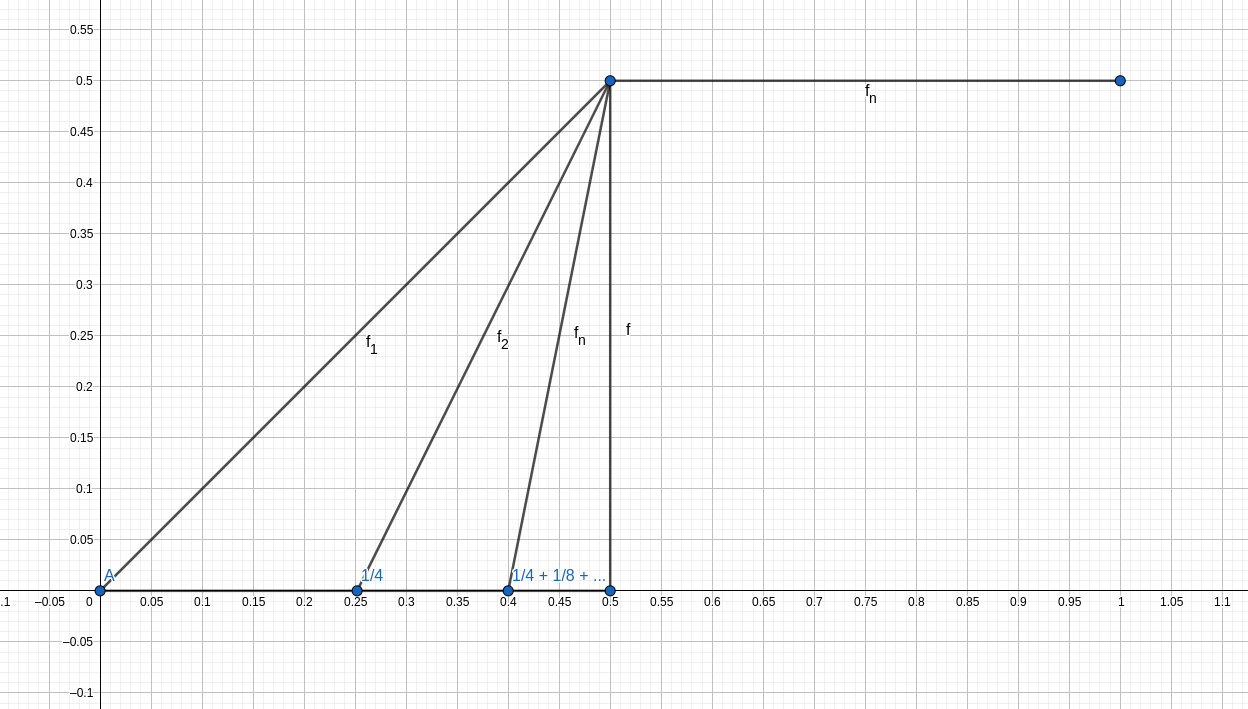
\includegraphics{figures/image_2020-06-29-20-40-22.png}

\begin{itemize}
\tightlist
\item
  Then each \(f_n\) is clearly integrable, since its graph is contained
  in the unit square.
\item
  \(\theset{f_n}\) is Cauchy: geometrically subtracting areas yields a
  single triangle whose area tends to 0.
\item
  But \(f_n\) converges to \(\chi_{[{1\over 2}, 1]}\) which is
  discontinuous.
\end{itemize}

\todo[inline]{show that $\int_0^1 \abs{f_n(x) - f_m(x)} \,dx \to 0$ rigorously, show that no $g\in L^1([0, 1])$ can converge to this indicator function.}

\end{solution}

\hypertarget{spring-2017-6}{%
\subsection{Spring 2017 \# 6}\label{spring-2017-6}}

Show that the space \(C^1([a, b])\) is a Banach space when equipped with
the norm
\begin{align*}
\|f\|:=\sup _{x \in[a, b]}|f(x)|+\sup _{x \in[a, b]}\left|f^{\prime}(x)\right|.
\end{align*}

\begin{solution}

Concepts used:

\begin{itemize}
\tightlist
\item
  See
  \url{https://math.stackexchange.com/questions/507263/prove-that-c1a-b-with-the-c1-norm-is-a-banach-space/}
\end{itemize}

\textbf{Solution}:

\begin{itemize}
\item
  Denote this norm \(\norm{\wait}_u\)
\item
  Let \(f_n\) be a Cauchy sequence in this space, so
  \(\norm{f_n}_u < \infty\) for every \(n\) and
  \(\norm{f_j - f_k}_u \converges{j, k\to\infty}\to 0\).
\end{itemize}

and define a candidate limit: for each \(x\in I\), set
\begin{align*}f(x) \definedas \lim_{n\to\infty} f_n(x).\end{align*}

\begin{itemize}
\item
  Note that
  \begin{align*} 
  \norm{f_n}_\infty &\leq \norm{f_n}_u < \infty \\
  \norm{f_n'}_\infty &\leq \norm{f_n}_u < \infty
  .\end{align*}

  \begin{itemize}
  \tightlist
  \item
    Thus both \(f_n, f_n'\) are Cauchy sequences in
    \(C^0([a, b], \norm{\wait}_\infty)\), which is a Banach space, so
    they converge.
  \end{itemize}
\item
  So

  \begin{itemize}
  \tightlist
  \item
    \(f_n \to f\) uniformly (by uniqueness of limits),
  \item
    \(f_n' \to g\) uniformly for some \(g\), and
  \item
    \(f, g\in C^0([a, b])\).
  \end{itemize}
\item
  Claim: \(g = f'\)

  \begin{itemize}
  \tightlist
  \item
    For any fixed \(a\in I\), we have
    \begin{align*}
    f_n(x) - f_n(a) \quad &\converges{u}\to f(x) - f(a) \\
    \int_a^x f'_n  \quad &\converges{u}\to \int_a^x  g
    .\end{align*}
  \item
    By the FTC, the left-hand sides are equal.
  \item
    By uniqueness of limits so are the right-hand sides, so \(f' = g\).
  \end{itemize}
\item
  Claim: the limit \(f\) is an element in this space.

  \begin{itemize}
  \tightlist
  \item
    Since \(f, f'\in C^0([a, b])\), they are bounded, and so
    \(\norm{f}_u < \infty\).
  \end{itemize}
\item
  Claim: \(\norm{f_n - f}_u \converges{n\to\infty}\to 0\)
\item
  Thus the Cauchy sequence \(\theset{f_n}\) converges to a function
  \(f\) in the \(u\dash\)norm where \(f\) is an element of this space,
  making it complete.
\end{itemize}

\end{solution}

\hypertarget{fall-2017-6}{%
\subsection{Fall 2017 \# 6}\label{fall-2017-6}}

Let \(X\) be a complete metric space and define a norm
\begin{align*}
\|f\|:=\max \{|f(x)|: x \in X\}.
\end{align*}

Show that \((C^0(\RR), \norm{\wait} )\) (the space of continuous
functions \(f: X\to \RR\)) is complete.

\begin{solution}

Concepts used:

\begin{itemize}
\tightlist
\item
  ??
\end{itemize}

\textbf{Solution}:

\begin{quote}
Should be supremum maybe..?
\end{quote}

Let \(\theset{f_k}\) be a Cauchy sequence, so \(\norm{f_k} < \infty\)
for all \(k\). Then for a fixed \(x\), the sequence \(f_k(x)\) is Cauchy
in \(\RR\) and thus converges to some \(f(x)\), so define \(f\) by
\(f(x) \definedas \lim_{k\to\infty} f_k(x)\).

Then
\(\norm{f_k - f} = \max_{x\in X}\abs{f_k(x) - f(x)} \converges{k\to\infty}\to 0\),
and thus \(f_k \to f\) uniformly and thus \(f\) is continuous. It just
remains to show that \(f\) has bounded norm.

Choose \(N\) large enough so that \(\norm{f - f_N} < \varepsilon\), and
write \(\norm{f_N} \definedas M < \infty\)

\begin{align*}
\norm{f} \leq \norm{f - f_N} + \norm{f_N} < \varepsilon + M < \infty
.\end{align*}

\end{solution}


\bibliography{/home/zack/Notes/library.bib}

\end{document}
